\documentclass[oneside,a4paper,spanish,links,12pt]{book}

\usepackage{fontspec} % alternativa a fontspec para luatex
\usepackage[utf8]{inputenc}
\usepackage{polyglossia}  % alternativa a babel para luatex

% Este es para agregar algoritmos y pseudocodigo
\usepackage[spanish,onelanguage,ruled,vlined,linesnumbered]{algorithm2e}

% estos dos son para poner figuras y figuras denotr de figuras
\usepackage{subcaption}
\usepackage{graphicx}
\usepackage[labelsep=period]{caption}

\usepackage{luacode}  % ejecutar lua en latex
\usepackage{pgfplots}  % para grafiacr con tablas dentro de latex

\usepackage{nomencl}  % imprimer la nomencltura
\usepackage{etoolbox}  % para agrupar la nomenclatura

\usepackage{amsmath}  % align environment

\usepackage{booktabs} % toprule, bottomrule, etc

\usepackage{hyperref}
% \usepackage{cleveref}
\usepackage[backend=biber,style=apa,citestyle=authoryear,hyperref=true]{biblatex}
% \usepackage[backend=biber,style=apa,hyperref=true]{biblatex}
\usepackage{geometry}

\usepackage{titlesec} % Permite cambiar el formato de los titulos
% \usepackage{times} % esta linea cambia fuente default LaTex a Times New Roman

\graphicspath{ {imagenes/} }

% ----------------------------------------------------------------------------
% Polylgossia
\setdefaultlanguage{spanish}
\addto\captionsspanish{\renewcommand{\tablename}{Tabla}}
\addto\captionsspanish{\renewcommand{\listtablename}{Índice de tablas}}

% ----------------------------------------------------------------------------
% fonts
% \setmainfont{Times New Roman}

% ----------------------------------------------------------------------------
% Nomenclature
% DE: https://www.overleaf.com/learn/latex/Nomenclatures
\renewcommand{\nomname}{Nomenclatura}
\renewcommand\nomgroup[1]{%
  \item[\bfseries
  \ifstrequal{#1}{G}{Geométricas}{%
  \ifstrequal{#1}{PO}{Parámetros Operativos}{%
  \ifstrequal{#1}{AG}{Algoritmo Genético}{%
  \ifstrequal{#1}{F}{Flujometrías}{}}}}%
]}

% Geometry
\geometry{a4paper, left=35mm, right=25mm,top=35mm,bottom=25mm,headsep=20mm}

% Luacode
\newcommand\lua[1]{\luaexec{#1}}


% ----------------------------------------------------------------------------
% Listings
% DE: https://www.overleaf.com/learn/latex/code_listing
\definecolor{codegreen}{rgb}{0,0.6,0}
\definecolor{codegray}{rgb}{0.5,0.5,0.5}
\definecolor{codepurple}{rgb}{0.58,0,0.82}
\definecolor{backcolour}{rgb}{0.95,0.95,0.92}
\usepackage{listings}
\lstdefinestyle{mystyle}{
    backgroundcolor=\color{backcolour},   
    commentstyle=\color{codegreen},
    keywordstyle=\color{magenta},
    numberstyle=\tiny\color{codegray},
    stringstyle=\color{codepurple},
    basicstyle=\ttfamily\footnotesize,
    breakatwhitespace=false,         
    breaklines=true,                 
    captionpos=b,                    
    keepspaces=true,                 
    numbers=left,                    
    numbersep=5pt,                  
    showspaces=false,                
    showstringspaces=false,
    showtabs=false,                  
    tabsize=2
}
\lstset{style=mystyle}

% ----------------------------------------------------------------------------
% Bibliografia - biblatex
\addbibresource{otros/bibliografia.bib}

% esta línea añade coma entre el autor y año de la referencia citada
\renewcommand*{\nameyeardelim}{\addcomma\space}

% ----------------------------------------------------------------------------
% hyperref
\hypersetup{
     colorlinks=true,
     linkcolor=blue,
     filecolor=blue,
     citecolor=blue,      
     urlcolor=red,
}

% ----------------------------------------------------------------------------
% biblatex y hyperref
\DeclareCiteCommand{\cite}
  {\usebibmacro{prenote}}
  {\usebibmacro{citeindex}%
   \printtext[bibhyperref]{\usebibmacro{cite}}}
  {\multicitedelim}
  {\usebibmacro{postnote}}

\DeclareCiteCommand*{\cite}
  {\usebibmacro{prenote}}
  {\usebibmacro{citeindex}%
   \printtext[bibhyperref]{\usebibmacro{citeyear}}}
  {\multicitedelim}
  {\usebibmacro{postnote}}

\DeclareCiteCommand{\parencite}[\mkbibparens]
  {\usebibmacro{prenote}}
  {\usebibmacro{citeindex}%
    \printtext[bibhyperref]{\usebibmacro{cite}}}
  {\multicitedelim}
  {\usebibmacro{postnote}}

\DeclareCiteCommand*{\parencite}[\mkbibparens]
  {\usebibmacro{prenote}}
  {\usebibmacro{citeindex}%
    \printtext[bibhyperref]{\usebibmacro{citeyear}}}
  {\multicitedelim}
  {\usebibmacro{postnote}}

\DeclareCiteCommand{\footcite}[\mkbibfootnote]
  {\usebibmacro{prenote}}
  {\usebibmacro{citeindex}%
  \printtext[bibhyperref]{ \usebibmacro{cite}}}
  {\multicitedelim}
  {\usebibmacro{postnote}}

\DeclareCiteCommand{\footcitetext}[\mkbibfootnotetext]
  {\usebibmacro{prenote}}
  {\usebibmacro{citeindex}%
   \printtext[bibhyperref]{\usebibmacro{cite}}}
  {\multicitedelim}
  {\usebibmacro{postnote}}

\DeclareCiteCommand{\textcite}
  {\boolfalse{cbx:parens}}
  {\usebibmacro{citeindex}%
   \printtext[bibhyperref]{\usebibmacro{textcite}}}
  {\ifbool{cbx:parens}
     {\bibcloseparen\global\boolfalse{cbx:parens}}
     {}%
   \multicitedelim}
  {\usebibmacro{textcite:postnote}}

% ----------------------------------------------------------------------------
% Formato de texto
\setlength{\parindent}{0.5cm}  % sangria de 0.5cm
\linespread{1.5}  % interlineado de 1.5pt
% la alineacion de latex viene justificada por defecto

% ----------------------------------------------------------------------------
% Formato de títulos (titlesec)

% Este conjunto de lineas cambia el tamaño de cada título
% \titleformat{command}[shape]{format}{label}{sep}{before}{afer}
\titleformat{\chapter}{\normalfont\large\bfseries}{\thechapter.}{20pt}{\large}
\titleformat{\section}{\normalfont\large\bfseries}{\thesection}{12pt}{\large}
\titleformat{\subsection}{\normalfont\large\bfseries}{\thesubsection}{12pt}{\large}
\titleformat{\subsubsection}{\normalfont\large\bfseries}{\thesubsubsection}{12pt}{\large}

% Este conjunto de lineas reduce el espacio entre título y texto
% \titlespacing{command}{left}{beforesep}{aftersep}{right}
\titlespacing*{\chapter}{0pt}{12pt}{6pt}
\titlespacing*{\section}{0pt}{12pt}{6pt}
\titlespacing*{\subsection}{0pt}{12pt}{6pt}
\titlespacing*{\subsubsection}{0pt}{12pt}{6pt}

\makenomenclature

\begin{document}

\begin{luacode}
dofile("data/data.lua")
\end{luacode}

%%%%%%%%%%%%%%%%%%%%%%%%%%%%%%%%%%%%%%%%%%%%%%%%%%%%%%%%%%%%%%%%%%%%%%%%%%%%%%%
% Caratula, resumen, indice, etc
\pagenumbering{roman}
\thispagestyle{empty}

\begin{center}

\Large\textbf{{Diseño de los sistemas de admisión y escape del Motor Rotativo de Combustión a Volumen Constante\\}}

\vspace{1cm}


\includegraphics[scale=0.65]{logo_unco.jpg}\\

\vspace{1cm}

\Large{\textbf{
NICOLÁS DANIEL BARRIOS\\
}}
\vspace{1cm}

PROYECTO INTEGRADOR PROFESIONAL\\

\vspace{1cm}

Presentado a la Facultad de Ingeniería de la Universidad Nacional del Comahue como requisito para la obtención del grado de \\ INGENIERO MECÁNICO

\vspace{0.5cm}

Neuquén - Argentina\\
AÑO 2024

\vspace{1cm}

\pagebreak
\thispagestyle{empty}

\Large\textbf{{Diseño de los sistemas de admisión y escape del Motor Rotativo de Combustión a Volumen Constante\\}}

\vspace{4cm}

\large{\textbf{
NICOLÁS DANIEL BARRIOS\\
}}

\vspace{4cm}
Director: Dr. Ing. \textbf{EZEQUIEL JOSÉ LÓPEZ}\\

% Co-director: Ing.  \textbf{NOMBRE DEL CO-DIRECTOR}

\vspace{3cm}
Presentado a la Facultad de Ingeniería de la Universidad Nacional del Comahue como requisito para la obtención del grado de \\ INGENIERO MECÁNICO

\vfill
Neuquén - Argentina

AÑO 2024

\newpage
\thispagestyle{plain}

\Large\textbf{{Diseño de los sistemas de admisión y escape del Motor Rotativo
    de Combustión a Volumen Constante \\}}

\vspace{3cm}

\large{\textbf{
NICOLÁS DANIEL BARRIOS
}}\\
\vspace{3cm}
\end{center}

Aprobado en fecha X de XXXXX de 2024

\vspace{2cm}

Tribunal evaluador:

\begin{itemize}

\item Dr. Ing. PRADO, Ricardo. %Miembro de mesa 1
\item Ing. ÁLVAREZ, Pablo. %Miembro de mesa 2
\item Ing. ZAPPA, Andrés. %Miembro de mesa 3
\item Mg. Ing. BOCCANERA, Daniel (Suplente). %Miembro de mesa 3
\end{itemize}

\newpage \thispagestyle{plain}

\begin{center} \large{\textbf{{Diseño de los sistemas de admisión y escape del
Motor Rotativo de Combustión a Volumen Constante}}}\\
\end{center} % \setstretch{1.5}

\normalsize \ \hfill Autor: Nicolás Daniel Barrios

\hfill Director: Dr. Ing. Ezequiel José López


\textbf{Resumen}

En este trabajo se optimizaron los sistemas de admisión y escape del Motor
Rotativo de Combustión a Volumen Constante (MRCVC) utilizando herramientas de
simulación computacional tales como ICESym (simulador 0D/1D de motores de
combustión interna), OpenFOAM (herramienta CFD de código abierto) y un
optimizador basado en un algoritmo genético (AG) desarrollado con la librería
DEAP (Python), entre otros.

Primero, se desarrolló una librería de funciones para acoplar el AG con ICESym,
permitiendo configurar, ejecutar y procesar datos del simulador.
%
También se modificó ICESym, agregando un modelo de coeficientes de descarga
($C_{D}$) dependiente de presión y apertura del puerto, permitiendo un mejor
modelado del flujo de gas a través de los puertos.

Se realizó una optimización inicial de la geometría de los puertos del MRCVC con
valores de $C_{D}$ constantes, buscando maximizar el rendimiento volumétrico.
%
La geometría resultante se modeló con un programa de diseño asistido por
computadora (CAD por sus siglas en inglés) de código abierto, FreeCAD.
%
Este resultado, junto con el estado termodinámico del gas obtenido de los datos
de salida de ICESym, se utilizó para realizar flujometrías virtuales de los
puertos en diferentes configuraciones empleando OpenFOAM, y así obtener el
correspondiente mapa de $C_{D}$.
%
Este mapa se utilizó como retroalimentación del AG para una nueva optimización,
logrando una geometría de puertos satisfactoria para el estado actual del motor.

\noindent

\textit{Palabras clave: MRCVC, Rendimiento volumétrico, Sistemas de intercambio
de gases, CFD, Optimización, Algoritmo Genético.}

\newpage \thispagestyle{plain} % \setstretch{1.0}

\begin{center} \large{\textbf{{Design of the Intake and Exhaust Systems of the
Constant Volume Combustion Rotary Engine}}}\
\end{center} % \setstretch{1.5}

\normalsize \hfill Author: Nicolás Daniel Barrios

\hfill Advisor: Dr. Ing. Ezequiel José López

\textbf{Abstract}

In this work, the intake and exhaust systems of the Constant Volume Combustion
Rotary Engine were optimized using computational simulation tools such
as ICESym (0D/1D internal combustion engine simulator), OpenFOAM (open-source
CFD tool), and a genetic algorithm (GA) based optimizer developed with the DEAP
(Python) library, among others.

First, a library of functions was developed to couple the GA with ICESym,
allowing configuration, execution, and data processing from the simulator.
%
ICESym was also modified to include a discharge coefficient ($C_{D}$) model
dependent on pressure and port opening, enabling better modeling of gas flow
through the ports.

An initial optimization of the engine port geometry was performed with constant
$C_{D}$ values, aiming to maximize volumetric efficiency.
%
The resulting geometry was modeled with an open-source computer-aided design
(CAD) program, FreeCAD.
%
This result, along with the gas thermodynamic state obtained from ICESym output
data, was used to conduct virtual flow measurements of the ports in different
configurations using OpenFOAM, thereby obtaining the corresponding $C_{D}$ map.
%
This map was used as feedback for the GA in a new optimization, achieving a
satisfactory port geometry for the current engine state.

\noindent

\textit{Keywords: MRCVC, Volumetric Efficiency, Gas Exchange Systems, CFD,
Optimization, Genetic Algorithm.}


\newpage

\tableofcontents \pagebreak
\listoffigures \pagebreak
\listoftables \pagebreak
% Los simbolos se arreglan como:
%
% G Geométricas
% PO Parámetros Operativos
% AG Algoritmo Genético
% F Flujometrías
% SU subindices

\nomenclature[G]{\(F_v\)}{Área efectiva de válvula}

%%%%%%%%%%%%%%%%%%%%%%%%%%%%%%%%%%%%%%%%%%%%%%%%%%%%%%%%%%%%%%%%%%%%%%%%%%%%%%%
\nomenclature[PO]{\(U\)}{Velocidad del fluido}
% \nomenclature[PO]{\(H_{vap}\)}{Entalpía de vaporización}
% \nomenclature[PO]{\(Q_{HVU}\)}{Poder calórico superior}

%%%%%%%%%%%%%%%%%%%%%%%%%%%%%%%%%%%%%%%%%%%%%%%%%%%%%%%%%%%%%%%%%%%%%%%%%%%%%%%
\nomenclature[AG]{\(N\)}{Cantidad de individuos}
\nomenclature[AG]{\(G\)}{Cantidad de generaciones}


%%%%%%%%%%%%%%%%%%%%%%%%%%%%%%%%%%%%%%%%%%%%%%%%%%%%%%%%%%%%%%%%%%%%%%%%%%%%%%%
\nomenclature[F]{\(C_{D,int}\)}{Coeficiente de descarga interpolado}
\nomenclature[F]{\(\theta\)}{Ángulo de ciclo}
 \printnomenclature \pagebreak
% % Los simbolos se arreglan como:
%
% G Geométricas
% PO Parámetros Operativos
% AG Algoritmo Genético
% F Flujometrías
% SU subindices

\nomenclature[G]{\(F_v\)}{Área efectiva de válvula}

%%%%%%%%%%%%%%%%%%%%%%%%%%%%%%%%%%%%%%%%%%%%%%%%%%%%%%%%%%%%%%%%%%%%%%%%%%%%%%%
\nomenclature[PO]{\(U\)}{Velocidad del fluido}
% \nomenclature[PO]{\(H_{vap}\)}{Entalpía de vaporización}
% \nomenclature[PO]{\(Q_{HVU}\)}{Poder calórico superior}

%%%%%%%%%%%%%%%%%%%%%%%%%%%%%%%%%%%%%%%%%%%%%%%%%%%%%%%%%%%%%%%%%%%%%%%%%%%%%%%
\nomenclature[AG]{\(N\)}{Cantidad de individuos}
\nomenclature[AG]{\(G\)}{Cantidad de generaciones}


%%%%%%%%%%%%%%%%%%%%%%%%%%%%%%%%%%%%%%%%%%%%%%%%%%%%%%%%%%%%%%%%%%%%%%%%%%%%%%%
\nomenclature[F]{\(C_{D,int}\)}{Coeficiente de descarga interpolado}
\nomenclature[F]{\(\theta\)}{Ángulo de ciclo}
 \printnomenclature \pagebreak

%%%%%%%%%%%%%%%%%%%%%%%%%%%%%%%%%%%%%%%%%%%%%%%%%%%%%%%%%%%%%%%%%%%%%%%%%%%%%%%
\pagenumbering{arabic}
% \addtocontents{toc}{\protect\setcounter{tocdepth}{2}}\pagebreak

\chapter{INTRODUCCIÓN} \label{capitulo:INTRODUCCION}
Este trabajo tiene el objetivo de obtener un diseño preliminar de la geometría
de los sistemas de intercambio de gases del Motor Rotativo de Combustión a
Volumen Constante~\parencite{toth}, con el objetivo general de maximizar la
eficiencia del sistema en un rango de velocidades del motor.
%

El MRCVC es un proyecto que surgió en la Universidad Nacional del Comahue,
presentado por Ingeniero Jorge A. Toth en el año 1996 al Instituto Nacional de
la Propiedad Industrial y patentado en el año 1999.

\begin{figure}
    \centering
    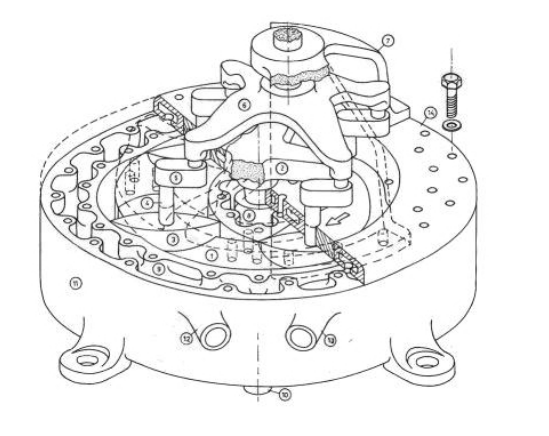
\includegraphics[width=0.5\textwidth]{perspectiva_mrcvc.png}
    \caption{Motor Rotativo de Combustión a Volumen Constante}\label{fig:mrcvc}
\end{figure}

En trabajos anteriores~\parencite{lopez16,lopez13}~se han mencionado
las características que hacen al MRCVC un motor atractivo: la geometría de la
cámara de combustión y del conjunto rotante permiten que gran parte del proceso
de combustión se realice a volumen constante, además de tener un balanceo
mecánico de fuerzas que le permite alcanzar altas velocidades de rotación.
%
Esto promete un funcionamiento más suave del motor, además de una reducción del
ruido y desgaste en comparación a motores rotativos tradicionales (Wankel) y
reciprocantes.
%
Por otro lado hay que mencionar que los motores rotativos traen consigo una
serie de problemas como la necesidad de introducir aceite a la cámara de
combustión para lubricar elementos móviles, el solape de cámaras durante la
apertura de los puertos y en particular al MRCVC un complejo sistema de
sellos~\parencite{roldan}.

%%%%%%%%%%%%%%%%%%%%%%%%%%%%%%%%%%%%%%%%%%%%%%%%%%%

La motivación de este trabajo surge del deseo de continuar con el desarrollo del
MRCVC y mejorar el pre-diseño de los sistemas de intercambio de gases, sentando
la base para una futura optimización de los mismos en un motor con requisitos de
diseño concretos.


Se buscó obtener un pre-diseño satisfactorio del sistema poniendo énfasis en la
geometría de los puertos de admisión y escape, definiendo las métricas a
utilizar para medir la eficiencia del sistema y poder realizar comparaciones
cuantitativas de los diseños propuestos.
%
% El prediseño consiste en definir las métricas a utilizar para medir la
% eficiencia del sistema, rea así como también poder comparar cualitativamente
% y cuantitativamente diferentes geometrías.
%
Debido al costo computacional de las simulaciones necesarias para realizar esta
optimización se restringe el modelado de la geometría a definir posiciones
angulares, largos y diámetros de los puertos.
%
No se repara en detalles como la forma de la transición entre las paredes del
puerto hacia la cámara de combustión, el ángulo al estator y detalles similares.

%%%%%%%%%%%%%%%%%%%%%%%%%%%%%%%%%%%%%%%%%%%%%%%%%%%
La optimización se realizó utilizando en conjunto una serie de herramientas de
simulación, de las cuales las principales fueron:

\begin{enumerate}
        %
    \item ICESym~\parencite{icesym}, simulador de motores de combustión interna basado en modelos cero-/uni-dimensionales (0D/1D).
        %
    \item OpenFOAM~\parencite{openfoam}, la herramienta libre de CFD.
        %
    \item Salome~\parencite{salome}, plataforma libre para simulación numérica.
        %
\end{enumerate}

\nomenclature[F]{\(CFD\)}{\textit{Computational Fluid Dynamics.}}

Se desarrolló un optimizador capaz de generar y evaluar diferentes geometrías
con el fin de buscar una combinación de parámetros que maximicen indicadores de
eficiencia del sistema, como por ejemplo, el rendimiento volumétrico del motor
para un rango de velocidades determinado.

El proceso de optimización consta de una primera aproximación utilizando como
punto de partida los resultados de trabajos anteriores~\parencite{lopez13}, en
los cuales se evaluó el funcionamiento del los parámetros que definen la
geometría de los sistemas de intercambio de gases, en particular: diámetros y
longitudes de conductos y reglaje o posición angular de los puertos.

La optimización se realiza con un algoritmo evolutivo (o genético) funcionando
en conjunto con ICESym, este último provee el puntaje a cada configuración del
motor necesario para estos procesos de optimización.
%
El puntaje se introduce en la función objetivo, la cual evalúa a cada uno de los
candidatos generados por el algoritmo.

El diseño preliminar de la primera ronda de optimización se volcó en un modelo
3D de los puertos, parametrizado de modo tal que se puede alterar rápidamente la
geometría, modificando variables como el diámetro de los conductos y la posición
relativa en la periferia del motor.
%
Este modelo 3D se utilizó para extraer la geometría a simular con OpenFOAM y
realizar flujometrías de las que se obtiene un valor del flujo másico
($\dot{m}$) en estado estacionario para un punto operativo del motor, es decir,
para una combinación de diferencia de presión entre puerto y cámara de
combustión ($\Delta P$) y el grado de apertura del puerto ($l_{v}$).
%
El flujo másico se utilizó para medir la eficiencia con la cual escurre el gas a
través del puerto, por medio del $C_{D}$ con el objetivo de crear un mapa del
coeficiente de descarga que sea función de las variables mencionadas.
%
Este mapa se utiliza como retroalimentación del simulador de motores ICESym,
para tener un mejor modelado del flujo de gas a través de los puertos en un
rango operativo del motor y con esto realizar una nueva corrida de optimización
para refinar el diseño obtenido en la primera iteración.
%
\nomenclature[PO]{\(\dot{m}\)}{Caudal másico}
\nomenclature[F]{\(C_{D}\)}{Coeficiente de descarga}

% Primer capitulo
La organización de este trabajo es como sigue.
%
En el presente capítulo se dio una introducción al trabajo, motivación y
objetivos del mismo.

% Segundo capitulo
En el segundo capítulo se da una breve descripción del funcionamiento de los
motores de combustión interna, seguido de los indicadores utilizados para medir
el rendimiento de motores en general e indicadores particulares de la
eficiencia de los sistemas de intercambio de gases, como el rendimiento
volumétrico y la fracción de gases residuales.
%
Luego, se describe el funcionamiento del MRCVC, indicando los aspectos que
hacen atractivo a este motor, además de desventajas del mismo y las posibles
aplicaciones.
%
También se describe el proceso de intercambio de gases y se define el
coeficiente de descarga $C_D$ y las ecuaciones asociadas.
%
Para finalizar el capítulo se presentan las flujometrías a realizar, modelos de
turbulencia utilizados y las condiciones iniciales y de contorno aplicadas en
las simulaciones.
%

En el tercer capítulo se describe la parte computacional del trabajo, se
presenta el simulador de motores \emph{ICESym}, el optimizador desarrollado y la
integración entre ambos programas.
%
Seguido de una descripción del funcionamiento del optimizador, los motivos de
seleccionar un algoritmo de tipo evolutivo o genético, las ventajas y
desventajas, los componentes básicos y finalmente la implementación del mismo.
%
En este capítulo también se presenta el software utilizado para realizar las
flujometrías, \emph{OpenFOAM}, la implementación de las condiciones iniciales y
de contorno, extracción de datos de ICESym y otras herramientas necesarias para
generar el modelo de CAD del puerto, malla y otros detalles relativos al proceso
de utilizar el programa.

% Cuarto capítulo
En el cuarto capítulo se presenta el desarrollo del trabajo, dando los resultados
de cada etapa.

% Quinto capítulo
Por último, se dan las conclusiones del trabajo, opiniones finales y una
perspectiva a futuro o posibles trabajos a seguir.
 \label{capitulo:1_INTRODUCCION} \pagebreak

\chapter{MARCO TEÓRICO} \label{capitulo:MARCO_TEORICO}
\section{Motores de combustión Interna}

\begin{figure} \centering 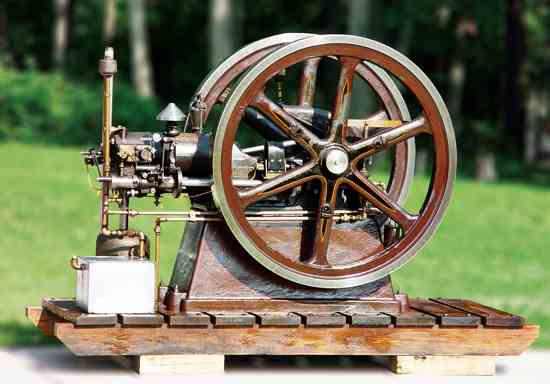
\includegraphics[width=.5\textwidth]{otto_1909.jpg}
    \caption{Motor 1909 5HP Otto Special Electric Lighting de Wayne
Grenning}\label{fig:otto1909} %
https://www.gasenginemagazine.com/gas-engines/1909-5-hp-otto-special-electric/
\end{figure}

Los motores de combustión interna dieron un impulso a la actividad humana desde
los años 1860, donde su uso comercial comenzó a popularizarse.
%
La función de estos dispositivos es la de convertir la energía potencial del
fluido de trabajo, una mezcla de aire-combustible, en trabajo mecánico por medio
de un proceso de combustión controlada dentro de un cilindro (cámara de
combustión).
%
Los primeros ejemplares comerciales eran voluminosos, costosos, altamente
ineficientes y de baja potencia, con valores de rendimiento cercano al 5\% y
potencias de hasta 6 HP.

Un paso importante hacia los motores actuales fue el desarrollo del ciclo Otto,
propuesto por Nicolaus A. Otto y Eugen Langen, cuyo primer prototipo se puso en
marcha en el año 1876.
%
Otto propuso un motor alternativo con cuatro carreras de pistón: admisión,
compresión, expansión y escape (ver figura \ref{fig:4tiempos}); este prototipo
lograba la misma potencia con mayor eficiencia que los motores de la época con
menos de la mitad del peso y volumen.
%
En la figura \ref{fig:otto1909} se ve un motor de ciclo Otto fabricado por
\emph{Otto Gas Engines Works} en el año 1909 en Filadelfia-EEUU, según la
revista \emph{Gas Engine
Magazine}\footnote{\url{https://www.gasenginemagazine.com/gas-engines/1909-5-hp-otto-special-electric/}}
\footnote{ \url{https://www.youtube.com/watch?v=LPSWfg0Y3Hs} } \footnote{
\url{https://www.youtube.com/watch?v=0d0WZ0H56_U} } este motor funcionaba
directamente acoplado a una bomba triplex de agua, como parte de un sistema de
irrigación de un club de campo de Delaware.
%
Los motores han continuado su desarrollo desde entonces, mejorando materiales,
combustibles y procesos de manufactura entre otros aspectos.
%
En las últimas décadas se ha hecho foco en disminuir el consumo de combustible,
el nivel de ruido, costo de manufactura, tamaño y las emisiones de gases de
efecto invernadero o contaminantes como las de $CO_2$, $CO$ y $NO_x$, entre
otras.



El ciclo operativo de cuatro tiempos de Otto se puede expresar en términos de
carreras del pistón, en la que pueden identificar dos posiciones de interés:
punto muerto superior (PMS) y el punto muerto inferior (PMI).
%
En el PMS se tiene el volumen mínimo atrapado en el cilindro y el pistón está al
final de la carrera, en el punto más alejado del eje del cigüeñal.
%
El PMI es el punto en el que se tiene el volumen máximo del cilindro y el pistón
está en el punto más cercano al eje del cigüeñal, como se ve en la
figura~\ref{fig:pms_pmi}.
%
Con esto en mente, el ciclo Otto de cuatro tiempos de un motor de encendido por
chispa se puede describir con cuatro carreras del pistón:
%
\begin{description}
%
    \item [Carrera de admisión] El pistón se mueve desde el PMS hasta el PMI con
la válvula de admisión abierta y la de escape cerrada, esto hace que ingrese una
masa de aire-combustible al cilindro.
%
    \item [Carrera de compresión] El pistón se mueve desde el PMI hacia el PMS
con la válvula de admisión y escape cerradas, esta reducción del volumen
comprime y calienta los gases en el interior del cilindro.
        %
        En una posición angular del ciclo conocida como avance de encendido se
enciende la mezcla.
%
    \item [Carrera de potencia o expansión] La combustión produce un aumento de
presión y temperatura en el cilindro, la carrera de expansión parte del PMS
hacia el PMI, aprovechando la expansión en volumen de los productos de la
combustión que producen trabajo sobre la cara del pistón.
%
    \item [Carrera de escape o barrido] Luego de la carrera de expansión, en el
PMI se abre la válvula de escape y el movimiento del pistón hacia el PMS produce
un barrido de los gases quemados.
%
\end{description}

\begin{figure}
  \centering
  \begin{subfigure}{0.6\textwidth}
    \centering
    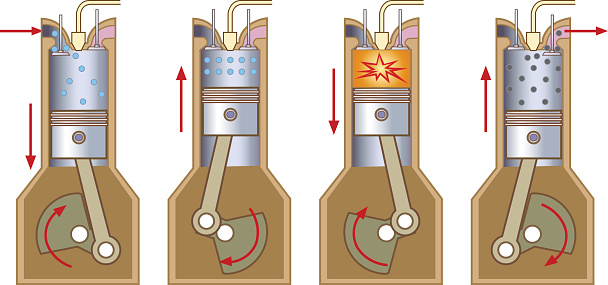
\includegraphics[width=\textwidth]{4stroke.jpg}
    \caption{Ciclo de cuatro tiempos}\label{fig:4tiempos} %
  \end{subfigure}%
  \begin{subfigure}{0.4\textwidth}
    \centering
    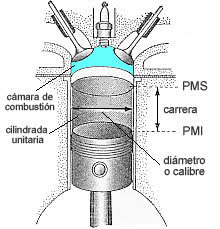
\includegraphics[width=\textwidth]{pms_pmi.jpg}
    \caption{PMS y PMI}\label{fig:pms_pmi}
  \end{subfigure}
  \caption{Ciclo de cuatro tiempos}
\end{figure}

% https://www.istockphoto.com/es/vector/motor-di%C3%A9sel-de-cuatro-tiempos-gm586705100-100702521

\subsection{Motores rotativos}
%
Los motores rotativos son una variable al diseño más popular de los motores
alternativos, su compacidad, balanceo y mayores velocidades de giro los vuelven
más atractivos en aplicaciones en las cuales el volumen es restringido.
%
La mayor velocidad de giro permite alcanzar mayores potencias por lo que tiene
una menor relación peso/potencia que motores reciprocantes de potencia similar.
%
El motor rotativo más conocido es el Wankel, cuyo primer prototipo funcional se
desarrolló cerca del 1957.
%
En la actualidad se cuenta con otros desarrollos de este tipo de motores como el
motor rotativo de pistón líquido, con un ciclo de combustión a volumen constante
denominado HECH\parencite{hehc_05}, similar al del MRCVC.

Si bien son una alternativa interesante a los motores reciprocantes, estos
motores requieren introducir aceite en la cámara de combustión para lubricar las
partes móviles, además tienen una mayor superficie de transferencia de calor por
lo que la pérdida de calor es mayor en comparación con los reciprocantes.
%
En la actualidad, los requisitos de niveles de emisiones ambientales de ciertos
gases hacen de estos motores inviables para el uso comercial, sin embargo la
compacidad del motor los vuelve atractivos en aplicaciones militares como por
ejemplo para vehículos aéreos no tripulados.

%%%%%%%%%%%%%%%%%%%%%%%%%%%%%%%%%%%%%%%%%%%%%%%%%%%%%%%%%%%%%%%%%%%%%%%%%%%%%%%


\subsection{Parámetros Operativos e Indicadores de rendimiento}
%
Para poder comparar entre diferentes diseños de motores se deben conocer algunos
parámetros operativos e indicadores de rendimiento, algunas de las
características más importantes de un motor son:
%
\begin{enumerate}
        %
    \item Potencia máxima
        %
    \item Torque máximo
        %
    \item Rango de velocidades de operación
        %
    \item Consumo de combustible, costo del combustible
        %
    \item Costo inicial, costo de operación, costo de mantenimiento
        %
    \item Confiabilidad
        %
    \item Ruido y emisiones contaminantes
        %
\end{enumerate}

% Estos aspectos permiten comparar entre diferentes alternativas de motores para
% decidir cuál es el que mejor aplica a la función que se le quiere dar.
%
Estas características se pueden expresar de manera más genérica en función de la
potencia, geometría u otros aspectos de un motor para obtener valores que se
pueden comparar directamente entre motores.
%
Por ejemplo, al cociente entre el trabajao entregado por ciclo y la cilindrada
de un motor se lo conoce como presión media efectiva o \emph{mep}, por sus
siglas en inglés.
%
Algunos parámetros operativos e indicadores se describen en los párrafos
siguientes.

%%%%%%%%%%%%%%%%%%%%%%%%%%%%%%%%%%%%%%%%%%%%%%%%%%%%%%%%%%%%%%%%%%%%%%%%%%%%%%%

\subsubsection{Volumen Desplazado}
%
El volumen desplazado se define como la diferencia entre el volumen máximo y
mínimo que ocupa la cámara de combustión.

\begin{equation}\label{eq:vol_desp} V_d = V_{max}-V_{min}
\end{equation}

% La geometría de la càmara de combustión del MRCVC está definida por leyeEn el
% MRCVC la geomeria de la cámara de combustión es m'0

%%%%%%%%%%%%%%%%%%%%%%%%%%%%%%%%%%%%%%%%%%%%%%%%%%%%%%%%%%%%%%%%%%%%%%%%%%%%%%%

\subsubsection{Relación de compresión}

Se define como el cociente ente el volumen máximo y el volumen mínimo del ciclo,
es uno de los parámetros más importantes de un motor ya que afecta la presión
máxima que se puede obtener en la cámara, la \emph{performance} potencia
entregada, esfuerzos mecánicos y rendimiento del motor.

\begin{equation}\label{eq:rel_comp} r_c = \frac{V_{max}}{V_{min}} = \frac{V_d+V_c}{V_c}
\end{equation}

%%%%%%%%%%%%%%%%%%%%%%%%%%%%%%%%%%%%%%%%%%%%%%%%%%%%%%%%%%%%%%%%%%%%%%%%%%%%%%%

% \subsubsection{Troque y potencia al freno} % NOTA: Hace flata?

%%%%%%%%%%%%%%%%%%%%%%%%%%%%%%%%%%%%%%%%%%%%%%%%%%%%%%%%%%%%%%%%%%%%%%%%%%%%%%%

\subsubsection{Trabajo indicado por ciclo}
%
El trabajo entregado por el cilindro al cigüeñal por cada ciclo de operación del
mismo se denomina trabajo indicado por ciclo y se obtiene al integrar la presión
en función del volumen, es el área encerrada en un diagrama de P-V del motor.

\begin{equation}\label{eq:w_indicado} W_{c,i} = \oint P dV
\end{equation}

Se debe diferenciar entre trabajo bruto y trabajo neto, en el último se tiene en
cuenta el trabajo de bombeo que resulta de la diferencia del trabajo realizado
durante las carreras de admisión y escape, por lo que este indicador se puede
diferenciar en:
%
\begin{description}
  \item [Trabajo bruto indicado por ciclo] $W_{c,ig}$, mide el trabajo realizado
por el motor en las carreras de compresión y expansión.
  \item [Trabajo neto indicado por ciclo] $W_{c,in}$, mide el trabajo realizado
por el motor considerando las 4 carreras del ciclo.
  \item [Trabajo de bombeo] La diferencia entre el trabajo bruto y neto es el
trabajo de bombeo $W_{bombeo}$ y mide el trabajo realizado durante los procesos
de admisión y escape.
  \item [Trabajo de fricción] Es el trabajo consumido por el rozamiento entre
partes móviles del motor.
\end{description}

% TODO, 15/07 agregar una figura con el área bajo la curva del diagrama P-V y si
% puedo indicar los trbajos de bombeo, bruto y neto, mejor

%%%%%%%%%%%%%%%%%%%%%%%%%%%%%%%%%%%%%%%%%%%%%%%%%%%%%%%%%%%%%%%%%%%%%%%%%%%%%%%

% \subsubsection{Rendimiento Mecánico}

%%%%%%%%%%%%%%%%%%%%%%%%%%%%%%%%%%%%%%%%%%%%%%%%%%%%%%%%%%%%%%%%%%%%%%%%%%%%%%%

\subsubsection{Consumo especifico de combustible y rendimiento de conversión de
combustible}
%
El consumo especifico de combustible \emph{sfc}, se define como el cociente
entre el caudal másico de combustible ($\dot{m_f}$) consumido por unidad de
potencia $P$ entregada por el motor.

\begin{equation}\label{eq:sfc} sfc = \frac{\dot{m_f}}{P}
\end{equation}

Mide la eficiencia con la que el motor utiliza el combustible para una condición
de operación dada, para motores de encendido por chispa se tienen valores
típicos para de alrededor de $65\mu g/J$.

Una versión similar de este indicador adimensionalizado en relación a la energía
suministrada por el combustible, es el \emph{rendimiento de conversión de
combustible} $\eta_f$, que se relaciona al \emph{sfc} por medio del poder
calórico del combustible, $Q_{HV}$.

\begin{equation}\label{eq:eta_f} \eta_f = \frac{1}{sfc \cdot Q_{HV}}
\end{equation}

El valor de $Q_{HV}$ es una propiedad del combustible que se determina en un
ensayo de laboratorio, valores típicos para los combustible comerciales basados
en hidrocarburos son 42 a 44 $MJ/kg$

%%%%%%%%%%%%%%%%%%%%%%%%%%%%%%%%%%%%%%%%%%%%%%%%%%%%%%%%%%%%%%%%%%%%%%%%%%%%%%%

\subsection{Presión Media Efectiva}
%
La presión media efectiva o $mep$ por sus siglas en inglés es un indicador cuya
variación es similar a la curva de torque pero adimensionalizada por el tamaño
de cada motor.
%
El trabajo realizado por ciclo se puede calcular como
$W_c = \frac{P \cdot n_r}{N}$, donde $n_R$ es el número de revoluciones del
cigüeñal por cada carrera de expansión por cilindro.
%
Para motores de cuatro tiempos $n_R=2$ y $n_R=1$ para motores de dos tiempos,
con esto la presión media efectiva se define como:

\begin{equation}\label{eq:mep} mep = \frac{W_{c}}{V_d} = \frac{P \cdot n_R}{V_d \cdot N}
\end{equation}

Se puede diferenciar entre presión media efectiva indicada (\emph{imep}), al
freno (\emph{bemp}) y de fricción (\emph{fmep}), utilizando el valor de potencia
correspondiente en la ecuación \ref{eq:mep}.
%
El valor de \emph{mep} (al igual que el torque) de un motor varía con la
velocidad de operación, siguiendo de cerca la curva de rendimiento volumétrico
como se puede ver en la figura~\ref{fig:bmep_tipica}.

En la actualidad, valores típicos de \emph{bmap} de motores SI naturalmente
aspirados rondan los 1050 a 1250 kPa para la velocidad a la que se alcanza el
torque máximo.

\begin{figure} \centering
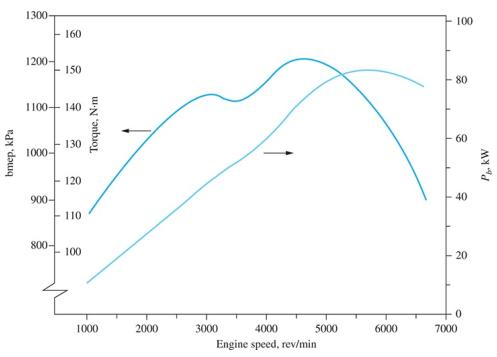
\includegraphics[width=0.7\textwidth]{curva_bmep_tipica.jpg}
    \caption{\emph{bmep}, torque y potencia vs velocidad de
operación\parencite{heywood}.}
    \label{fig:bmep_tipica}
\end{figure}

%%%%%%%%%%%%%%%%%%%%%%%%%%%%%%%%%%%%%%%%%%%%%%%%%%%%%%%%%%%%%%%%%%%%%%%%%%%%%%%

\subsection{Rendimiento Volumétrico}
%
El rendimiento volumétrico mide la eficiencia del sistema de admisión y se
define como el cociente entre el caudal másico de aire que ingresa al sistema de
admisión y la velocidad con la que este volumen es desplazado por el pistón.
%
En otras palabras, este indicador mide la eficiencia con la que el motor bombea
aire.

\begin{equation}\label{eq:eta_v} \eta_v = \frac{2\dot{m_a}}{\rho_{a,i}V_d N} = \frac{m_a}{\rho_{a,i}V_d}
\end{equation}

Para motores naturalmente aspirados, la densidad del aire de admisión
$\rho_{a,i}$ se toma comúnmente como la densidad atmosférica por lo que $\eta_v$
mide el rendimiento de todo el sistema de admisión.

El valor de rendimiento volumétrico máximo para motores naturalmente aspirados
ronda el 90\%.
%
Su valor se ve afectado por varios fenómenos dentro de los cuales los más
importantes son:

\begin{description}
        %
    \item [Efectos cuasiestáticos] Combustible, relación aire/combustible,
vaporización del combustible en el conducto de admisión, temperatura del aire de
admisión, relación entre presión de admisión y escape, relación de compresión,
etc.
  \item [Pérdidas de carga por fricción viscosa] Las pérdidas viscosas aumentan
con la velocidad de flujo y aumentan a medida que aumenta la velocidad de giro
del motor.
        %
  \item [Pérdidas de carga localizada] Filtros, puertos, válvulas generan
pérdidas localizadas, caídas de presión.
        %
  \item [Transferencia de calor en sistema de admisión] La mezcla se calienta
por transferencia de calor y esto disminuye la densidad de la misma, reduciendo
la masa disponible para la combustión.
        %
  \item [Reglaje de las válvulas/puertos] El punto de apertura y cierre de los
puertos (reglaje) es clave para el funcionamiento del motor, dependiendo del
reglaje que se elija, se puede favorecer el flujo a determinada velocidad de
operación.
        %
    \item [Flujo bloqueado en puertos de admisión y escape] En las zonas de
menor área de pasaje la velocidad del fluido puede aumentar hasta alcanzar la
velocidad del sonido, esto se conoce como bloqueo y limita el caudal másico que
puede ingresar a la cámara de combustión.
        %
%     \item [Transferencia de calor en el cilindro] La cámara de combustión se %
encuentra a mayor temperatura que la mezcla que ingresa, esto produce un aumento
% del volumen específico reduciendo la cantidad que puede ingresar.
        %
    \item [Sintonía del puerto de admisión y escape] El diseño de los puertos de
admisión y escape puede favorecer el funcionamiento de los mismos a determinada
velocidad de operación, esto se logra aprovechando las ondas de presión que se
producen por la apertura y cierre de las válvulas.
        %
  \item [Sobrecarga] Por medio de un compresor o turbocompresor se puede
aumentar presión en el sistema de admisión forzando más aire a la cámara de
combustión.
        %
    \item [Efecto RAM] A grandes velocidades de flujo la inercia del gas produce
un aumento de presión al momento del cierre del puerto de admisión y esto
permite un mayor ingreso de masa fresca al cilindro.
        %
\end{description}

La curva de rendimiento volumétrico es muy similar a la curva de torque o de
presión media efectiva, la cantidad de aire que ingresa al motor está
directamente relacionada con el de trabajo que se puede realizar por cada ciclo
de operación.
%
% Esto se ve claramente en un motor de inyección directa, donde la cantidad de %
combustible a inyectar está limitada por la masa de aire fresca en la cámara de
% combustión, siempre que se mante.
%
Este indicador es central en la evaluacion del desempeño de los sistemas de
intercambio de gases y es el principal indicador utilizado en este trabajo y
buscó que el software desarrollado devuelva un espectro de opciones de
configuración de los puertos, de los cuales seleccionar la mejor geometría
teniendo en cuente este y otros indicadores de rendimiento y parámetros
operativos en general, como lo son el torque y la potencia entegada.
%
% Analizar detalladamente los efectos que hacen al valor final de $\eta_v$ es de
% una complejidad que excede a este trabajo, en su lugar se buscó maximizar %
$\eta_v$ sin entrar en detalle de los efectos presentes.

En este trabajo se busco que la curva de rendimiento volumétrico de los motores
simulados tenga un máximo para velocidades mayores a 6000 RPM para de aprovechar
el balanceo mecánico del motor que permite funcionar y seguir entreganto
potencia a altas RPM además, se la curva debe ser suave para todo el régimen de
funcionamiento del motor.
%
% y que la fracción de % % gases residuales se mantenga baja en todo el régimen
de funcionamiento del % motor.

% Se buscó una curva de rendimiento volumétrico con un máximo para altas %
revoluciones de modo de aprovechar el balanceo del motor para maximizar el
trabajo % realizado a altas velocidades para obtener potencias altas a altas
RPM, a su vez % se buscó mantener valores de fracción de gases residuales $x_r$
relativamente % bajas..
%
Estos efectos se describen en detalle en la literatura\parencite{heywood}, para
este trabajo se tiene las siguientes consideraciones:

\begin{enumerate}
        %
    \item El combustible utilizado es isooctano, la mezcla aire-combustible es
estequeométrica ($\phi=1$).
        %
    \item El sistema de intercambio de gases del MRCVC se compone de un conducto
y puerto admisión, conducto y puerto de escape.
        %
        El software ICESym tiene en cuenta pérdidas por fricción viscosa en los
conductos y los puertos son los únicos elementos que generan pérdidas
localizadas.
        %
    \item Los conductos se asumen como elementos rectos de un largo finito y
diámetro constante, cuya fuente y sumidero es la atmósfera a $101330.0 Pa$ y
$25^{\circ}C$.
        %
    \item La temperatura de la pared de la cámara de combustión se asume en
450K.
        %
    \item El motor es naturalmente aspirado.
        %
\end{enumerate}

\subsection{Fracción de gases residuales}
%
La fracción de gases residuales $x_r$ mide la cantidad de gases quemados que hay
en el cilindro al inicio de la carrera de admisión.
%
Esto ocurre principalmente por dos razones, en primer lugar queda gas atrapado
en el cilindro, remanente del ciclo anterior y en segundo lugar puede existir un
reflujo desde el puerto de escape hacia la cámara de combustión si hay solape de
válvulas, lo que afecta: rendimiento volumétrico, trabajo obtenido, eficiencia y
emisiones.

En el MRCVC existe además solape de cámara, este es un fenómeno en el que una
cámara en proceso de admitir gases frescos se ve afectada por la apertura del
puerto de admisión a la cámara siguiente, que se encuentra a mayor presión y
temperatura por estar culminando el proceso de escape y comenzando el de
admisión, esto reduce el rendimiento volumétrico.
%
% Un esquema de este proceso se puede ver en la figura \ref{fig:reflujo_solape}.
% falta la figura
%
\subsection{Coeficiente de descarga}
%
La pérdida de carga localizada en los puertos de admisión y escape se puede
medir con el coeficiente de descarga $C_{D}$, este indicador mide la eficiencia
del escurrimiento y se obtiene experimentalmente o con simulaciones
computacionales.
%
El valor de $C_{D}$ varía con la geometría y condiciones de operación del
puerto, siendo $C_{D}=1$ el caso ideal sin pérdida de carga localizada.

El caudal másico que fluja o circula por los puertos se calcula a partir de las
ecuaciones de flujo compresible a través de una restricción, para el caso en que
el flujo no esté bloqueado la ecuación de $\dot{m}$ es
la~\ref{eq:m_no_bloqueado} y en caso de que se cumpla la
desigualdad~\ref{eq:condicion_bloqueo} el flujo está bloqueado y se utiliza la
ecuación~\ref{eq:m_bloqueado}.
%

\begin{equation}\label{eq:m_no_bloqueado} \dot{m} = \frac{C_D A_R p_0}{\sqrt{R T_0}} {\left(\frac{p_T}{p_0} \right)}^{1/\gamma} {\left( \frac{2\gamma}{\gamma-1} \left[1- {(\frac{p_T}{p_0})}^{{\gamma-1}/\gamma} \right] \right)}^{1/2}
\end{equation}

\begin{equation}\label{eq:condicion_bloqueo} \frac{p_T}{p_0} \le {[\frac{2}{\gamma+1}]}^{\gamma/(\gamma - 1)}
\end{equation}

\begin{equation}\label{eq:m_bloqueado} \dot{m}=  \frac {C_D A_R p_0} {{(R T_0)}^{1/2}} \gamma^{1/2} {\left( \frac{2\gamma}{\gamma+1} \right)}^{(\gamma+1)/(2(\gamma-1))}
\end{equation}

Dónde:

\begin{itemize}
    \item $p_0$, es la presión de estancamiento antes de la restricción.
    \item $T_0$, es la temperatura de estancamiento antes de la restricción.
    \item $p_T$, es la presión estática justo después de la restricción.
    \item $A_R$, es el área de pasaje de flujo o de referencia.
    \item $\dot{m}$, es el caudal másico.


  \item $\gamma$, es el cociente de capacidades térmicas del gas.
\end{itemize}

Presiones y temperaturas se pueden medir u obtener de una simulación
computacional del ciclo del motor.
%
La elección del área de referencia utilizada para el cálculo es arbitraria, sin
embargo se suele utilizar el área de cortina, que se calcula como con el
producto del diámetro $D_{v}$ y alzada de válvula $l_{v}$.

\begin{equation} \label{eq:area_cortina} A_R = A_C = \pi D_v l_v
\end{equation}

\begin{figure} \centering
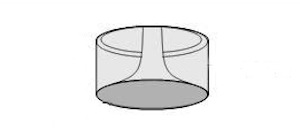
\includegraphics[width=0.5\textwidth]{valve_curtain.jpg}
  \caption{Área de cortina}\label{fig:area_cortina}
\end{figure}


%%%%%%%%%%%%%%%%%%%%%%%%%%%%%%%%%%%%%%%%%%%%%%%%%%%%%%%%%%%%%%%%%%%%%%%%%%%%%%%
% \subsection{Sistema de intercambio de gases} % % % En un motor típicio de
combustión interna el sistema de intecambio de gases se % compone de una toma de
aire, filtro de aire, cuerpo de mariposa, puerto de % admisión.  % % % Por parte
del escape se tiene un puerto de escape, catalizador y silenciador % hasta
descargar en la atmósfera.  % % % Como se mencionó en el apartado anterior, para
este trabajo es utilizó un % sistema simplificado en el que solamente se tiene
conducto de admisión y escape % junto con puertos de admisión y escape.

%%%%%%%%%%%%%%%%%%%%%%%%%%%%%%%%%%%%%%%%%%%%%%%%%%%%%%%%%%%%%%%%%%%%%%%%%%%%%%%

\subsection{Sincronización del sistema de admisión}
%
% Al abrir el puerto de admisión se pone en contacto los gases residuales de la
% cámara de combustión con la masa fresca en el puerto de admisión, estos dos %
volúmenes se encuentran a diferente presión que tiende que tiende a
%
En motores naturalmente aspirados, al momento de abrir la válvula o puerto de
admisión, los gases residuales en la cámara se encuentran a una presión mayor
que la masa fresca en el puerto de admisión, esta diferencia de presión produce
una onda de depresión que viaja desde la cámara de combustión hacia el extremo
opuesto del conducto de admisión.
%
Cuando esta onda de presión llega al plenum de admisión, se refleja como una
onda de sobrepresíon que toma un tiempo $t$ en alcanzar nuevamente el puerto, si
el tiempo que toma la onda en reflejarse es tal que alcanza la válvula justo
antes del cierre de la misma se dice que el puerto el sistema está sintonizado.
%
Esta sopbrepresión permite que ingrese una mayor cantidad de masa fresca a la
cámara de combustión, aumentando la cantidad de trabajo que se puede realizar.

En la figura~\ref{fig:sintonia1} se muestra el diagrama de presión vs ángulo de
cigüeñal para 1200 y 4800 RPM, en donde se indican los períodos en los que se
encuentran abiertos las válvulas de admisión (IO) y de escape (EO).
%
Los valores $p_1$, $p_2$ y $p_3$ hacen referencia diferentes longitudes de los
conductos de admisión y escape.
%
Se puede ver que para $p_1$ a 4800 RPM hay un claro pico de presión justo al
cierre del puerto de admisión, con esto el puerto está sintonizado para esta
velocidad.

\begin{figure} \centering
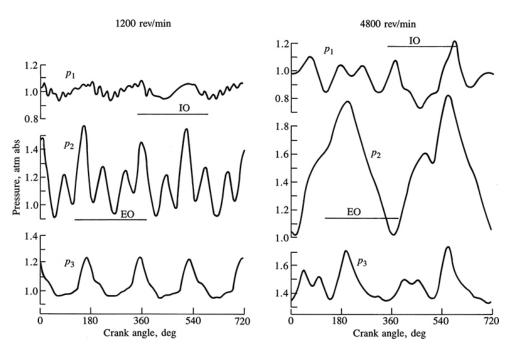
\includegraphics[width=0.7\textwidth]{sintonia_heywood.jpg}
    \caption{(cambiar por una del mrcvc) Diagrama de presión vs ángulo de
cigüeñal}\label{fig:sintonia1}
\end{figure}

Debido a que la onda de presión debe viajar dos veces longitud del conducto de
admisión desde el momento que abre el puerto de admisión, para sincronizar el
sistema de admisión a bajas velocidades, se requieren longitudes mayores lo que
hace más grande el sistema de admisión.
%
La sincronía a mayores velocidades de admisión es preferida, porque usualmente
se tiene el máximo de torque y de potencia a mayores RPM, además reduce la
necesidad de conductos mámás largos.
%
En motores multi cilíndricos se utiliza un plenum de admisión, este dispositivo
proporciona un volumen grande de aire que se utiliza como resonador.
%
Se puede hacer vibrar de modo que las oscilaciones de presión internas envían
ondas de sobre presión a cada puerto en el momento preciso en el que se aproxima
el cierre del mismo.

%%%%%%%%%%%%%%%%%%%%%%%%%%%%%%%%%%%%%%%%%%%%%%%%%%%%%%%%%%%%%%%%%%%%%%%%%%%%%%%

\subsection{Sincronización del sistema de escape}

De forma análoga al puerto de admisión, al momento de la apertura del puerto o
válvula de escape los gases residuales de la combustión se encuentran a una
mayor presión que el gas en el conducto, esto crea una onda de sobrepresión que
viaja por el escape hasta alcanzar el final del mismo o un área de gran volumen,
como el catalizador o el silenciador.
%
Desde esta zona se refleja como una onda de depresión, que si alcanza el puerto
justo antes del cierre del mismo ayuda a evacuar una mayor cantidad de gas,
disminuyendo la cantidad de gases residuales presentes para el próximo ciclo.

Reducir la cantidad de gases residuales tiene dos efectos beneficiosos, en
primer lugar estos gases ocupan volumen en la cámara de combustión, además
porque su elevada temperatura (en relación a la masa fresca) calienta el gas que
ingresa al cilindro desde el puerto de admisión, aumentando el volumen
específico y reduciendo el rendimiento volumétrico.

En la figura \ref{fig:sintonia1} se ve que para el escape en $p_2$ se tiene una
depresión justo al cierre del puerto, este sistema está sintonizado para 4800
RPM, es notorio el contrate con el mismo puerto a 1200 RPM, en donde se ve un
pico de presión cerca del cierre del puerto.

%%%%%%%%%%%%%%%%%%%%%%%%%%%%%%%%%%%%%%%%%%%%%%%%%%%%%%%%%%%%%%%%%%%%%%%%%%%%%%%

\subsection{Combustión}
%
La combustión es un proceso en el que se libera la energía química del
combustible, la geometría de un motor de combustión interna permite aprovechar
el aumento de presión y temperatura que ocurre en la cámara durante este proceso
para convertir esta energía en trabajo mecánico.
%
Los modelos ideales de ciclos operativos se pueden clasificar según el proceso
de combustión en:
%
\begin{enumerate}
        %
    \item volumen constante
        %
    \item presión constante
        %
    \item presión limitada (parte a volumen constante y parte a presión
constante)
        %
\end{enumerate}

En un motor de encendido por chispa se tiene una mezcla de aire-combustible en
la cámara de combustión, dependiendo del tipo de motor la mezcla se puede formar
en el conducto de admisión, inyectando combustible en algún punto del sistema ó
se puede producir la mezcla en la cámara por la inyección directa de
combustible.
%
En un motor de encendido por compresión, la mezcla combustible se forma en la
cámara de combustión, luego de la inyección directa del combustible.

\begin{figure}
  \centering
  \begin{subfigure}{0.33\textwidth}
    \centering
    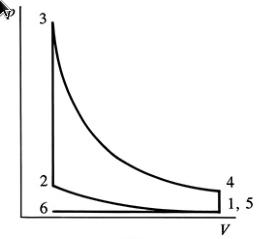
\includegraphics[width=\textwidth]{combustion_vol_cte.jpg}
    \caption{Combustión a Volumen Constante}
  \end{subfigure}%
  \begin{subfigure}{0.33\textwidth}
    \centering
    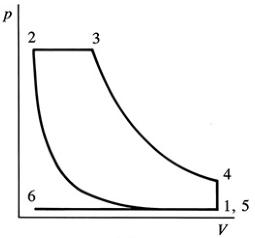
\includegraphics[width=\textwidth]{combustion_presion_cte.jpg}
    \caption{Combustión a Presión Constante}
  \end{subfigure}%
  \begin{subfigure}{0.4\textwidth}
    \centering
    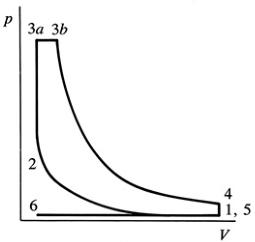
\includegraphics[width=\textwidth]{combustion_presion_limitada.jpg}
    \caption{Combustión a Presión Limitada}
  \end{subfigure}
  \caption{Diagramas P-V para ciclos ideales\parencite{heywood}}\label{fig:ciclos_ideales}
\end{figure}

El MRCVC es un motor de combustión interna encendido por chispa en el que,
gracias al a geometría del mismo gran parte de la combustión ocurre a volumen
constante, esto se puede apreciar en la apreciar en la
figura~\ref{fig:vol_constante}, la cual es una gráfica de volumen obtenida de
una de las simulaciones del MRCVC con ICESym.
%
En este trabajo no se estudia el proceso de combustión del MRCVC, sin embargo se
describe el motivo por el que la combustión a volumen constante es una
característica atractiva de este motor.  % es más eficiente que la combustión a
presión constante.

En \parencite{heywood} se hace un análisis de los modelos operativos de gas
ideal, en los cuales se asume que % El mayor rendimiento de la combustión a
volumen constante se puede ver % analizando los modelos ideales de ciclos
operativos \parencite{heywood}, el fluido de trabajo es gas ideal, con $C_v$ y
$C_p$ constantes.
%
Se pueden analizar los 3 casos de combustión: volumen constante, presión
constante o presión limitada, obteniendo expresiones para el rendimiento de
conversión de combustible~\ref{eq:rendimiento_p_lim} y de $imep$ en función de
la presión mínima del ciclo $p_1$~\ref{eq:imep_p1} y máxima
$p_3$~\ref{eq:imep_p3}.
%
Tanto la combustión a volumen constante como el caso a presión constante son
casos extremos de la combustión a presión limitada, por lo que se puede utilizar
el rendimiento de conversión de combustible para el ciclo de presión limitada es
para comparar entre ambos.

\begin{align}
    \label{eq:rendimiento_p_lim}
    %
    \eta_{f,i} &= 1 - \frac{1}{r_c^{\gamma - 1}} \left[ \frac{\alpha \beta^\gamma-1}{\alpha \gamma (\beta-1)+\alpha-1} \right]\\ \alpha &= \frac{P_3}{P_2}\\ \beta &= \frac{V_{3b}}{V_{3a}}
    %
\end{align}

\begin{equation}
    \label{eq:imep_p1} \frac{imep}{p_1} = \frac{Q^*}{c_v T_1 (\gamma-1)} \left( \frac{r_c}{r_c-1} \right) \eta_{f,i}
    %
\end{equation}

\begin{equation}
    \label{eq:imep_p3} \frac{imep}{p_3} = \frac{1}{\alpha r_c^\gamma} \left( \frac{Q^*}{c_v T_1} \right) \left(\frac{1}{\gamma-1} \right) \left( \frac{r_c}{r_c-1} \right) \eta_{f,i}
    %
\end{equation}

En el caso en que  $\alpha=1 \rightarrow P_3=P_2$ y se tiene el ciclo de
combustión a presión constante, en el caso en que
$\beta=1 \rightarrow V_{3a}=V_{3b}$ y se tiene el ciclo de combustión a volumen
constante, como se ve en la figura \ref{fig:ciclos_ideales}.

Graficando la ecuación \ref{eq:rendimiento_p_lim} en función de la relación de
compresión $r_c$ (figura \ref{fig:rendimientos}), para distintos valores se ve
que a igual relación de compresión, el ciclo a volumen constante presenta mayor
rendimiento de conversión de combustible.

Del mismo modo, graficando la relación entre la presión media efectiva indicada
y la presión máxima del ciclo, $imep/p_3$, se ve que a igual relación de
compresión el ciclo de combustión a presión constante presenta mayores valores
de $imep$ en relación a la presión máxima, esto tiene que ver con las altas
presión alcanzadas en el ciclo ideal de combustión a volumen constante.
%
La presión máxima que se puede alcanzar en el ciclo real tiene limitaciones
relacionadas a mayores pérdidas de masa (y presión) a través de sellos y la
resistencia mecánica de los componentes del motor además, mayores presiones
están asociadas con mayores temperaturas en la cámara de combustión.

\begin{figure} \centering
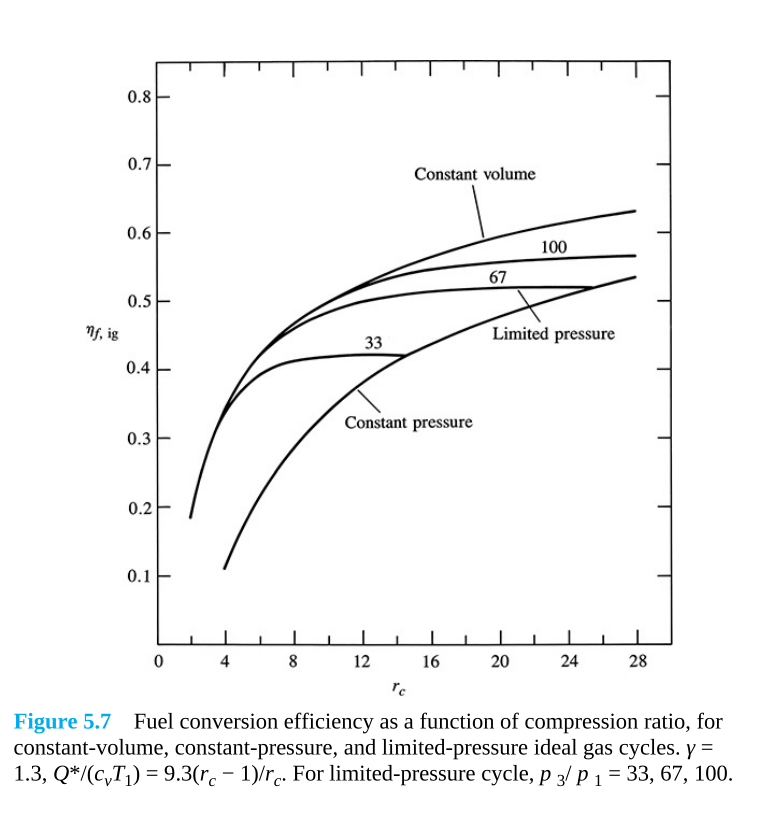
\includegraphics[width=.7\textwidth]{rendimiento_conv_comb.png}
    \caption{Rendimiento de conversión de combustible en función de $r_c$ para
ciclos de gas ideal de volumen constante, presión constante y presión
limitada(cambiar por propia??)} \label{fig:rendimientos}
    %
\end{figure}


\subsection{Propiedades termodinámicas de mezclas aire-combustible}\label{subsec:prop_mezcla}
%
La combustión de una mezclas de aire-combustible es la fuente de energía del
motor, se debe poder calcular con cierto grado de certeza las propiedades
termodinámicas del fluido de trabajo a lo largo del ciclo de operación.
%
En lo pertintente a este trabajo, el simulador ICESym contiene rutinas
computacionales para calcular el estado del fluido de trabajo en el ciclo
operativo del motor el por lo que este aspecto esta cubierto, sin embargo fue
necesario estimar las propiedades termodinámicas de la mezcla para obtener
algunas variables utilizadas para calcular las condiciones iniciales del gas en
las flujometrías.

Hay extensa literatura sobre el tema por lo que en este apartado simplemente se
detallan las hipótesis y modelos utilizados en las rutinas computacionales.

En la simulación del MRCVC se utilizó una mezcla estequeométrica de
aire-isooctano $C_{8}H_{18}$ cuya reacción estequeométrica se indica en la
ecuación \ref{eq:estequeometrica}, este combustibles es normalemente usado en
investigación de motores de combustión interna es el combustible de referencia
utilizado para determinarl el octanaje de un motor.

\begin{equation} \label{eq:estequeometrica}
  C_{8}H_{18} + 12.5 \left(O_{2}+3.772N_{2}\right) \rightarrow 8 CO_{2} + 9 H_{2}O + 47.16 N_{2}
\end{equation}

Expresando el combustible de manera genérica com $C_{a}H_{b}$ o en función de la cantidad
de moles de carbono del combustible $CH_{y}$, se puede expresar la proporción estequeométrica
de aire combustible que se requeieren como se ve en la ecuación~\ref{eq:rel_as}

\begin{equation} \label{eq:rel_as}
  \left(\frac{A}{F}\right)_{s} = \left(\frac{F}{A}\right)_{s}^{-1} = \frac{34.56(4+y)}{12.011 + 1.008y}
\end{equation}


Otro número importante es la relación de equivalencia que se calcula con el
cociente entre la relacion molar real y estequeométrica de una mezcla, ver
ecuación~\ref{eq:phi}

\begin{equation}\label{eq:phi}
  \phi = \frac{{(F/A)}_{real}}{{(F/A)}_{s}}
\end{equation}

Para calcular las propiedades teromdinámicas de las mezclas aire-combustible se
utilizaron rutinas computacionales que aproximan las mismas con curvas
polinómicas asumiendo que: 1) la composición de la mezcla sin quemar está,
congelada 2) la mezcla de gases quemados se encuentra en equilibrio químico.

La composición de la mezcla no cambia significativamente durante los procesos de
admisión y compresión, por lo que se asume que la mezcla está congelada.
%
Durante la combustión y parte del proceso de expansión se asume que la mezcla de
gases quemados está cerca del equilibrio termodinámico, a medida que los gases
se enfrían en durante la expansión, se puede asumir que la composición química
se congela.

Para cada compuesto $i$ a temperatura estándar T(K) y 1 atmósfera de presión se
aproxima el calor especifico a presión constante $\widetilde{c_{p,i}}$ por la
ecuación~\ref{eq:cp}, la entalpía estándar $\widetilde{h_{i}}$ por la
ecuación~\ref{eq:h} y la entropía estándar $\widetilde{s_{i}}$ por la
ecuación~\ref{eq:s}.

\begin{equation}\label{eq:cp} \frac{\widetilde{c_{p,i}}}{T} = a_{i1} + a_{i2}T + a_{i3}T^{2} + a_{i4}T^{3} + a_{i5}T^{4}
\end{equation}

\begin{equation}\label{eq:h} \frac{\widetilde{h_{i}}}{\widetilde{R}T} = a_{i1} + \frac{a_{i2}}{2}T + \frac{a_{i3}}{3}T^{2} + \frac{a_{i4}}{4}T^{3} + \frac{a_{i5}}{5}T^{4} +\frac{a_{i6}}{T}
\end{equation}


\begin{equation}\label{eq:s} \frac{\widetilde{s_{i}}}{\widetilde{R}} = a_{i1} \ln{T} + a_{i2}T + \frac{a_{i3}}{2}T^{2} + \frac{a_{i4}}{3}T^{3} + \frac{a_{i5}}{4}T^{4} + a_{i6}
\end{equation}

La base de datos seleccionada para los datos del aire y productos de la
combustión es Chemkin~\parencite{chemkin} y los datos del isooctano de
Raine~\parencite{raine}.

La finalidad de estas rutinas (por fuera de las incuidas en ICESym) es la de
obtener la masa molar de la mezcla $M_{M}$, la viscosidad dinámica, calor
específico a presión constante $C_{P}$, gamma $\gamma$ y el número de Prandtl
$P_{R}$, utilizados para algunos valores iniciales de las flujomerias.

La masa molar de la mezcla $M_{M}$ se calcula a partir de la suma de las masas
molares $M_{i}$ y la fracicón molar de cada especie química presente en la
mezcla $x_{i}$, ver ecuación~\ref{eq:mw}.
%
La viscosidad dinámica $\mu$ de productos de la combustión de de mezclas de aire-combustible se
aproxima a partir de la relación de equivalencia
de la mezcla $\phi$ y la temperatura $T$ en Kelvins, ver

La viscosidad $\mu$ de los productos de la combustión de aire e hidrocarburos
para temperaturas de entre $T\in [500, 4000]K$, $P\in[1, 100]atm$ y
$\phi \in [0,4]$ se puede aproximar en función de la temperatura y la relación
de equivalencia con la ecuación~\ref{eq:mu}.
%
Del mismo modo, el número de Prantl de productos de la combustión de
hidrocarburos y aire se puede estimar en función del $\gamma$ de la mezcla, para
$\phi\leq 1$ con la  ecuación~\ref{eq:pr}

\begin{equation}\label{eq:mw}
  Mm = \sum_{i} M_{i}x_{i}
\end{equation}

\begin{equation}\label{eq:mu}
  \mu_{productos} = \frac{\mu_{aire}} {1 + 0.027 \phi} = \frac{3.3\times 10^{-7} T^{0.7}} {1 + 0.027 \phi}
\end{equation}

\begin{equation}\label{eq:pr}
    Pr = 0.05 + 4.2 (\gamma - 1) - 6.7 {(\gamma - 1)}^{2}
\end{equation}
 \label{capitulo:2_MCI} \pagebreak
\section{Geometría y Ciclo Operativo del MRCVC}
%
En este apartado se describen algunos de los aspectos geométricos del motor y
ciclo operativo del MRCVC.

Los componentes principales del motor son: rotor, estator, paletas, bieletas,
rueda paralelizadoras, eje de motor, conducto de admisión y conducto de escape;
el motor analizado en este trabajo tiene 3 paletas con ápices agudos, que
corresponden a la geometría ideal del motor (con ápices de paletas de radio
nulo).
%
La forma de estos elementos se puede ver en la figura~\ref{fig:mrcvc} y en la
tabla~\ref{tab:geom_mrcvc} se resume el valor de los parámetros geométricos que
utilizados en este trabajo.

% Para un motor de $n$ paletas de radio de punta nulo, la geometría como función
% del ángulo del cigüeñal queda totalmente definida por el radio de trayectoria
% de paletas $R$, semi ancho de paletas $r$ y altura de cámara $h$.

Uno de los aspectos más importantes de este motor es la geometría de la cámara
de combustión, su forma es tal que el volumen mínimo del ciclo permanece
constante por un período angular considerable, determinado por la geometría del
motor.
%
Este período es lo suficientemente grande para permitir que la combustión se
realice casi en su totalidad a volumen constante.
%

La combustión a volumen constante brinda una mejora en el rendimiento energético
del motor además, el balanceo de fuerzas que se obtiene por ser un motor
rotativo permite operar el motor a altas RPM y así alcanzar mayores potencias
que motores de tamaño o cilindrada similar.
%
Esta combinación de un rendimiento y potencia que, en principio pueden ser altos
en comparación a motores cilindrada similar, hace atractivo el desarrollo de
este motor.
%
En la figura \ref{fig:ciclo_pv_mrcvc} se presenta el diagrama $P-V$ de una
simulación de ICESym del MRCVC.


\begin{figure}[ht]
  \centering
  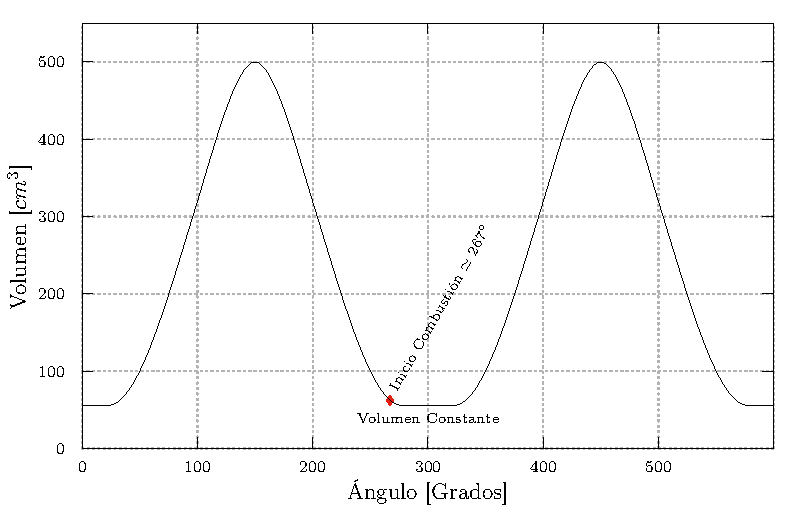
\includegraphics[width=\textwidth]{gnuplot/vol.pdf}
  \caption{Diagrama P-V del MRCVC}\label{fig:ciclo_pv_mrcvc}
\end{figure}

\begin{figure}[ht]
  \centering
  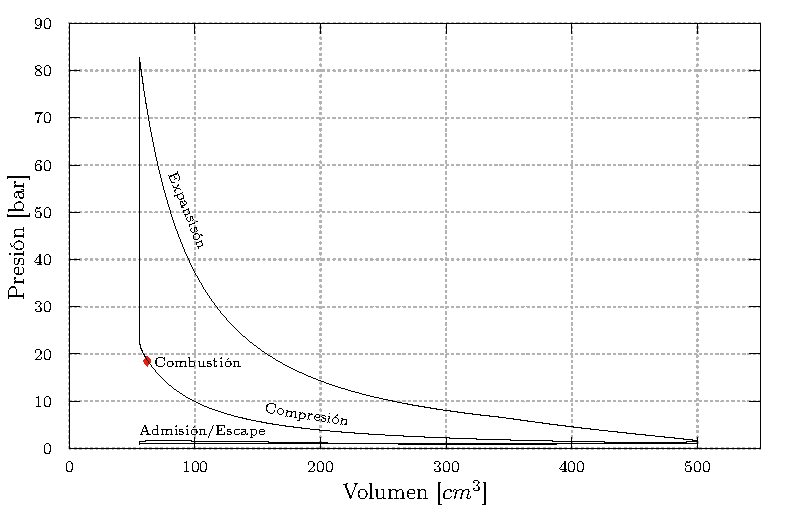
\includegraphics[width=\textwidth]{gnuplot/vol_vs_pres.pdf}
  \caption{Ciclo operativo del MRCVC}\label{fig:ciclo_mrcvc}
\end{figure}


El ciclo operativo del MRCVC es un ciclo Otto en el que las carreras de
admisión, compresión, expansión y escape ocurren a medida que el fluido de
trabajo rota con respecto al eje del cigüeñal.
%
En la figura~\ref{fig:ciclo_mrcvc} se puede ver una progresiva del ciclo del
MRCVC con estas carreras representadas en azul para la admisión, compresión en
amarillo, la expansión en rojo y escape o barrido en violeta.

Durante el ciclo se destaca un aspecto particular de este motor, siguiendo la
paleta de color negro se ve que durante el proceso de compresión y combustión,
las paletas que forman la frontera aguas arriba y aguas abajo de la cámara de
combustión cambian.
%
La paleta que delimitaba el frente de la cámara se retrasa con respecto a la
cámara con la que inició el ciclo, produciendo que este dure más de 1 revolución
resultando en aproximadamente 600º.

Para un motor de $R=\lua{tex.print(myData.R)}$ mm y
$r=\lua{tex.print(myData.r)}$ mm  el volumen mínimo alcanzado permanece
constante por un período de $44.65^\circ$, como se puede ver en la
figura~\ref{fig:vol_constante} en donde se esquematiza la variación del volumen
con respecto al ciclo.

% \begin{figure}
%     \centering
%     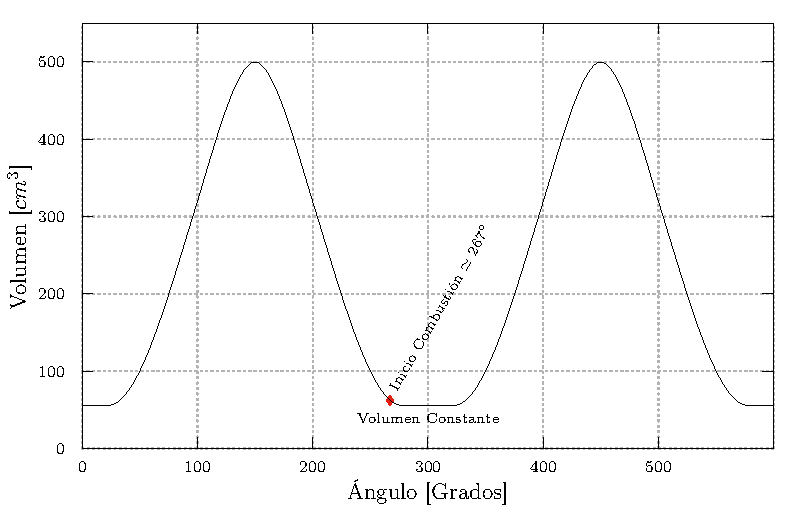
\includegraphics[width=\textwidth]{gnuplot/vol.pdf}
%     \caption{Variación del volumen del MRCVC de 3 paletas}\label{fig:vol_constante}
% \end{figure}

\begin{table}
    \centering
    \begin{tabular}{r|cccccccc} \toprule
     Parámetro & n & R & r & $h_c$ & rc & V0 & $R_i$ & $R_e$ \\ \midrule
     Valor & \lua{tex.print(myData.n)} & \lua{tex.print(myData.R)} & \lua{tex.print(myData.r)} & \lua{tex.print(myData.hc)} & \lua{tex.print(myData.rc)} & \lua{tex.print(myData.V0)} & \lua{tex.print(trunc(myData.Ri))} & \lua{tex.print(trunc(myData.Re))} \\
     Unidades & --- & mm & mm & mm & --- & $cm^3$ & mm & mm \\ \bottomrule
    \end{tabular}
    \caption{Geometría del MRCVC}\label{tab:geom_mrcvc}
\end{table}

% %%%%%%%%%%%%%%%%%%%%%%%%%%%%%%%%%%%%%%%%%%%%%%%%%%%%%%%%%%%%%%%%%%%%%%%%%%%%%%%
%
% \subsection{Geometría}
% %
% La geometría del MRCVC permite que gran parte de la combustión se de a volumen
% constante\parencite{mrcvc_geom}, como se puede ver en la figura~\ref{fig:vol_constante},
% en donde se esquematiza la variación del volumen con respecto al ciclo.
%
% \begin{figure}
%     \centering
%     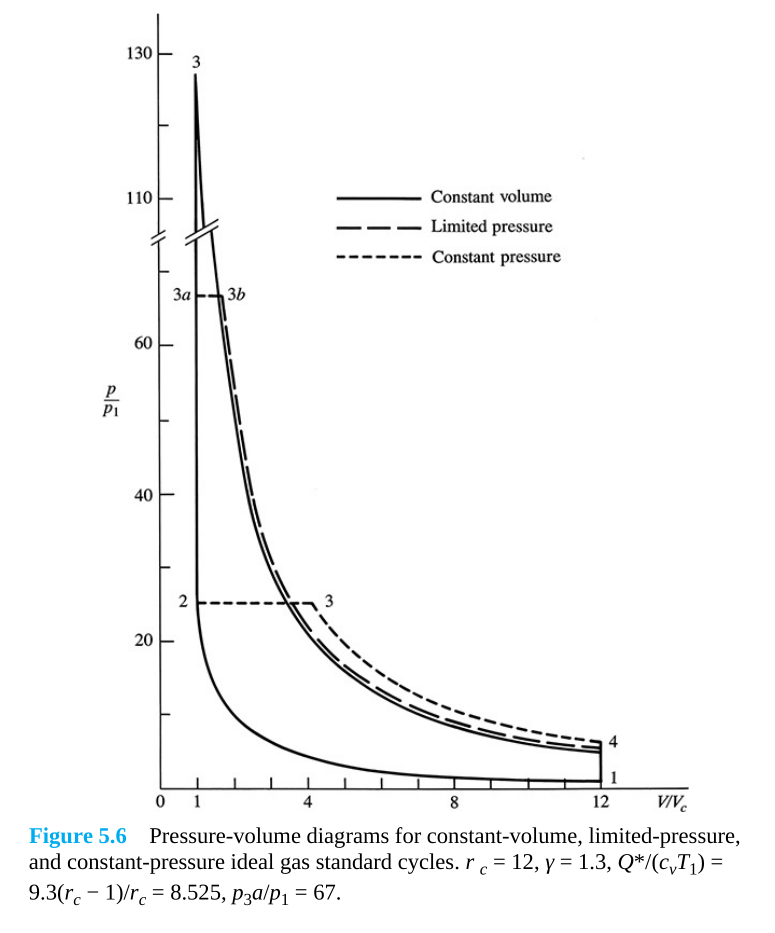
\includegraphics[width=0.7\textwidth]{comparacion_ciclos.png}
%     \caption{Comparación de ciclos ideales (cambiar por una imagen propia)}\label{fig:comparacion_ciclos}
% \end{figure}
%
%
% Para un motor de $n$ paletas de radio de punta nulo, la geometría como función
% del ángulo del cigüeñal queda totalmente definida por el radio de trayectoria de
% paletas $R$, semi ancho de paletas $r$ y altura de cámara $h$.
%
% \begin{figure}
%     \centering
%     \begin{tikzpicture}
%         \begin{axis}[
%             xlabel=Angulo $(deg)$,
%             ylabel=Volumen $(mm^3)$,
%             grid=major,
%             mark size=0pt,
%         ]
%         \addplot table [x=Angle,y=Volume] {data/vol.dat};
%         \end{axis}
%     \end{tikzpicture}
%     \caption{Combustión a volumen constante}\label{fig:vol_constante}
% \end{figure}
%
% La geometría utilizada para este trabajo se resumen en la
% tabla~\ref{tab:geom_mrcvc} y se ilustra en la figura~\ref{fig:geom_mrcvc}.
% %
% Esta geometría es la continuación de la utilizada en trabajos anteriores, con la
% cual se realizó parte del prediseño del sistema de intercambio de gases.
%
% \begin{table}
%     \centering
%     \begin{tabular}{rcc} \toprule
%         Parámetro & Valor                            & Unidades \\ \midrule
%         n         & \lua{tex.print(myData.n)}        & unidades \\
%         R         & \lua{tex.print(myData.R)}        & mm \\
%         r         & \lua{tex.print(myData.r)}        & mm \\
%         $h_c$     & \lua{tex.print(myData.hc)}       & mm \\
%         rc        & \lua{tex.print(myData.rc)}       & --- \\
%         V0        & \lua{tex.print(myData.V0)}       & $cm^3$ \\
%         $R_i$     & \lua{tex.print(trunc(myData.Ri))} & mm \\
%         $R_e$     & \lua{tex.print(trunc(myData.Re))} & mm \\
%     \end{tabular}
%     \caption{Geometría del MRCVC}\label{tab:geom_mrcvc}
% \end{table}
%
% Los ángulos que determinan el reglaje de los puertos de admisión y escape son los
% de inicio y de cierre del puerto.
% %
% Como ejemplo, la posición del puerto de escape queda determinada por los  valores
% EIA y EFA como se ve en la figura~\ref{fig:angulos_escape}.
%
% \begin{figure}
%     \centering
%     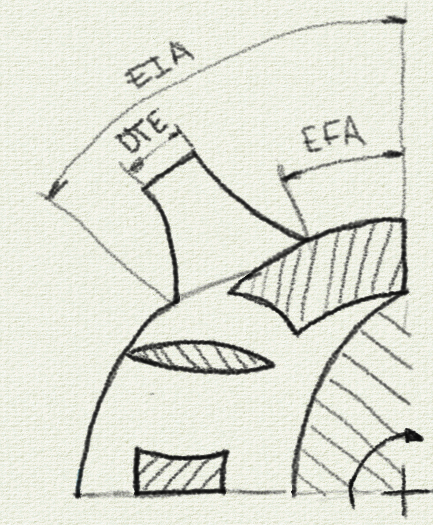
\includegraphics[width=0.5\textwidth]{angulos_escape.png}
%     \caption{Puerto de escape}\label{fig:angulos_escape}
% \end{figure}
%
% % NOTA: esto deberia ir en la parte de geometria de los puertos, luego de la
% % primer iteracion de opttimizacion
%
% % Como se puede ver en la figura~\ref{fig:primeros_puertos}, se buscó suavizar los
% % vértices en donde la pared del puerto intersecta la cámara de combustión.
%
% %%%%%%%%%%%%%%%%%%%%%%%%%%%%%%%%%%%%%%%%%%%%%%%%%%%%%%%%%%%%%%%%%%%%%%%%%%%%%%%
%
% \subsection{Ciclo operativo}
% %
% La variación de la geometría y el funcionamiento en detalle de ICESym, así como
% también el modelo de solape de cámaras desarrollado para el uso con el MRCVC.\@
% %
% Para una misma relación de compresión, una combustión a volumen constante
% alcanza valores de presión y temperatura mayores en comparación a otros ciclos.
% %
% En la figura~\ref{fig:comparacion_rendimientos} se ve como para una $r_c$ dada,
% el ciclo a volumen constante tiene el mayor rendimiento.
%
% \begin{figure}
%     \centering
%     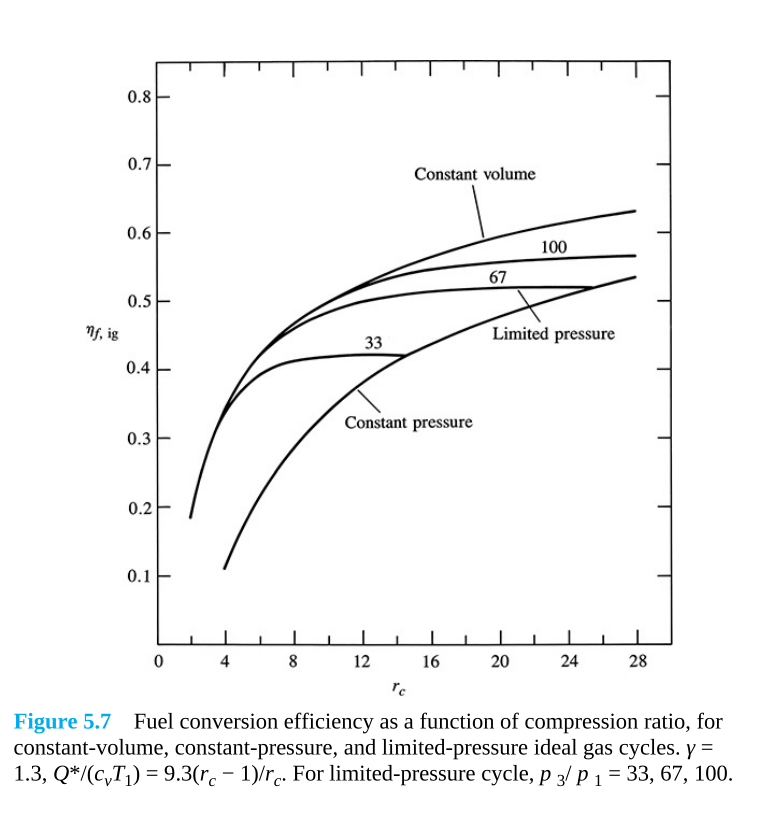
\includegraphics[width=1\textwidth]{rendimiento_conv_comb.png}
%     \caption{Comparación de rendimientos (cambiar por una imagen propia)}\label{fig:comparacion_rendimientos}
% \end{figure}
%
% El indicador que se tomará como referencia para evaluar y comparar diferentes
% geometrías es el rendimiento volumétrico ($\eta_v$), este parámetro se define
% como:
%
% \begin{equation}
%     \eta_v = \frac{m_a}{\rho_{a,i}V_d}
% \end{equation}
%
% Dónde:
% %
% \begin{description}
%     %
%     \item[$m_i$] es la masa de mezcla fresca inductada
%         %
%     \item[$\rho_{a,i}$] es la densidad del aire en el puerto de admisión
%         %
%     \item[$V_d$] es el volumen desplazado
%         %
% \end{description}
%
% El rendimiento volumétrico tiene una dependencia compleja de varios factores,
% este parámetro es el que da forma a las curvas de \emph{performance} que se
% suelen ver en literatura ya que indica la cantidad de mezcla fresca disponible
% para la combustión. 
% %
% % En caso de motores de inyección directa (tanto de CI SI)
% % NOTA: no se que quise poner aca, voy a tener que leerlo con mas de talle de
% % nuevo
%
% La combustión es estequeométrica con $a_{weibe}=5$ y $m_{weibe}=2$, el combustible utilizado
% es \emph{isooctano} con las siguientes características:
% \begin{itemize}
%     \item $y = 2.25$
%     \item $H_{vap} = 2.25 MJ/kg$
%     \item $Q_{fuel} = 44 MJ/kg_f$
% \end{itemize}
%
% La temperatura de pared se asume en 450K.

%%%%%%%%%%%%%%%%%%%%%%%%%%%%%%%%%%%%%%%%%%%%%%%%%%%%%%%%%%%%%%%%%%%%%%%%%%%%%%%

\subsection{Sistemas de intercambio de gases}
%
En un motor típico de combustión interna el sistema de intecambio de gases se
compone de una toma de aire, filtro de aire, cuerpo de mariposa, puerto de
admisión, puerto y conducto de escape, catalizador y silenciador hasta
finalmente descargar en la atmósfera.

Para simplificar el sistema analizado, no se tuvieron en cuenta elementos como:
mariposa, carburador,filtros de aire, convertidores catalíticos y demás;  sino
que se utilizó un sistema simplificado en el que solamente se tiene conducto de
admisión y escape junto con puertos de admisión y escape.
%
El eje de los conductos coincide con el eje del puerto, estos últimos hacen una
transición desde el diámetro del conducto hasta la altura de la ranura del
puerto en la cámara de combustión, en la
figura~\ref{fig:sistema_intercambio_gases} se esquematiza la geometría
mencionada.

\begin{figure}
    \centering
    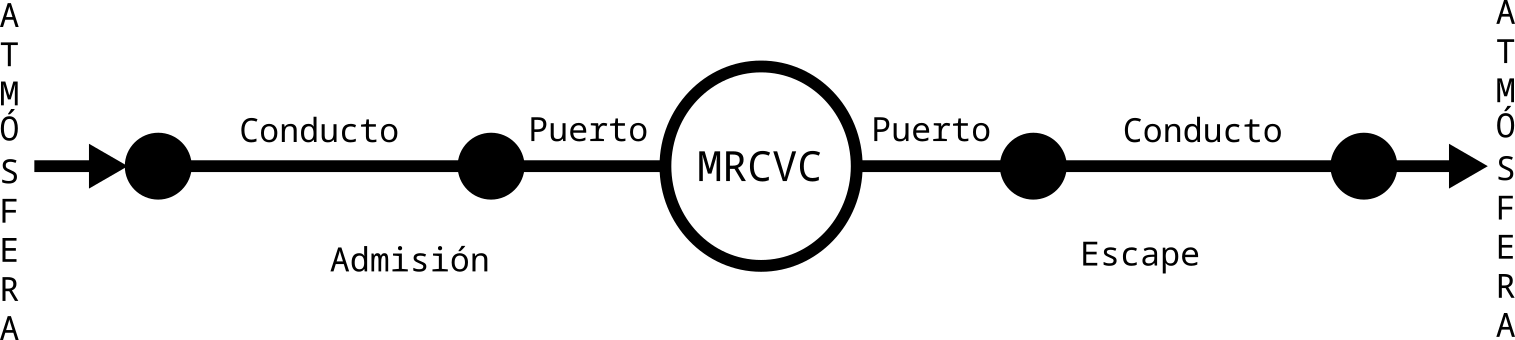
\includegraphics[width=\textwidth]{ciclo/sistema_intercambio_gases.png}
    \caption{Esquema del sistema de intercambio de gases}\label{fig:sistema_intercambio_gases}
\end{figure}


En trabajos anteriores~\parencite{lopez13} se demostró que se tiene una mejor
\emph{performance} del motor si se ubican los puertos en el cuerpo central del
estator.
%
En dicho trabajo se realizó una optimización de la geometría mediante un barrido
paramétrico de las variables que determinan la forma, posición y reglaje de los
puertos, ya que es la ubicación angular de los puertos la que determina la
duración de los procesos de admisión y escape.
%
% Los ángulos que determinan el reglaje de los puertos de admisión y escape son
% los de apertura y de cierre del puerto.
%
Los puertos de admisión y escape están fijos en en la periferia del estator y su
posición se indica con los ángulos \emph{IIA}, e \emph{IFA} para la admisíon y
\emph{EIA} y \emph{EFA} para el escape.
%
En la figura~\ref{fig:angulos_escape} se indican estos para el puerto de escape.

\begin{figure}
    \centering
    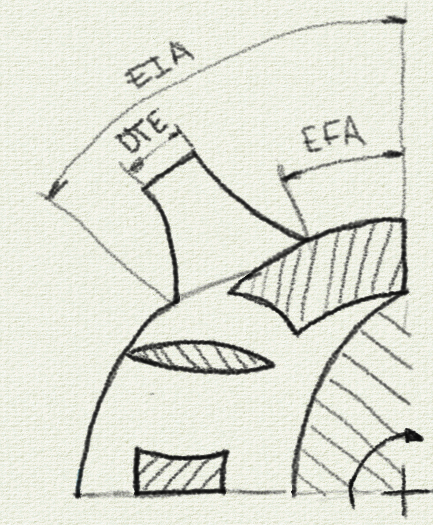
\includegraphics[width=0.5\textwidth]{angulos_escape.png}
    \caption{Puerto de escape}\label{fig:angulos_escape}
\end{figure}
 \label{capitulo:2_MRCVC} \pagebreak
%%%%%%%%%%%%%%%%%%%%%%%%%%%%%%%%%%%%%%%%%%%%%%%%%%%%%%%%%%%%%%%%%%%%%%%%%%%%%%
% Flujoemtrias y cfd
%%%%%%%%%%%%%%%%%%%%%%%%%%%%%%%%%%%%%%%%%%%%%%%%%%%%%%%%%%%%%%%%%%%%%%%%%%%%%%
 \label{capitulo:2_CFD} \pagebreak

\chapter{HERRAMIENTAS COMPUTACIONALES} \label{capitulo:HERRAMIENTAS_COMPUTACIONALES}
\section{Internal Combustion Engine Simulator}
%
ICESym es un simulador de motores de combustión interna que  utiliza modelos 0D
para la cámara de combustión y 1D para el flujo a través del sistema de
intercambio de gases.
%
Esta combinación permite evaluar la \emph{performance} de un motor a un costo
computacional relativamente bajo; además la implementación de entrada y salida
de datos facilita utilizar el simulador como una \emph{caja negra}.
%
Esta característica permite incluir al simulador en un \emph{script} como una
función, a la cual se le otorga un conjunto de parámetros de entrada y devuelve
los resultados de la simulación en un formato que permite la lectura y
evaluación de los mismos.

ICESym contiene en su código las rutinas necesarias para simular el ciclo
operativo y la geometría del MRCVC.
%
Se realizaron modificaciones menores para facilitar la ejecución en conjunto con
el optimizador, algunas de estas modificaciones fueron:
%
\begin{enumerate}
    \item Modificar el formato de los archivos de salida, con el fin de reducir
el tamaño de los archivos de salida, facilitar la lectura y el procesamiento de
datos.
    \item Incluir una opción para elegir entre un modelo de $C_D$ de una o dos
variables.
    \item Modificar el área de referencia, ver ec.\ref{eq:fv}
    \item Agregar un esquema de interpolación bilineal que permita tabajar con
el modelo de $C_{D}$ de dos variables.
\end{enumerate}


\section{Modificaciones a ICESym}
%%%%%%%%%%%%%%%%%%%%%%%%%%%%%%%%%%%%%%%%%%%%%%%%%%%%%%%%%%%%%%%%%%%%%%%%%%%%%%%
\subsection{Flujo a Través de los Puertos}
%
Se introdujo una opción para poder ejecutar ICESym con un modelo del coeficiente
de descarga que dependa de dos variables: diferencia de presión y \emph{alzada}
o apertura del puerto, $C_D = f(lv; \Delta P)$.
%
Esto significó agregar un \emph{switch} en el código que permita seleccionar
entre un modelo de una o dos variables, con el agregado de las instrucciones de
lectura de datos y armado de un arreglo bidimensional que contiene los valores
del mapa de $C_{D}$ en un orden dado.
%
Con esto se construye un mapa del coeficiente de descarga de la forma $C_D =
f(lv, \Delta P)$, que se utiliza para calcular el área efectiva del puerto.

\nomenclature[F]{\(\Delta P\)}{Diferencia de presión a través de un puerto}


Independientemente de la cantidad de variables que formen parte del coeficiente
de descarga, a ICESym se introduce un vector para el caso 1D y matriz para el
caso 2D.
%
El esquema de interpolación bilineal implementado requiere de una malla
rectangular, se reutilizó el código existente para el caso 1D y se realiza una
interpolación lineal entre dos valores en planos con datos conocidos, como se ve
en la Figura~\ref{fig:interp_bilineal}.

\begin{figure}
    \centering
    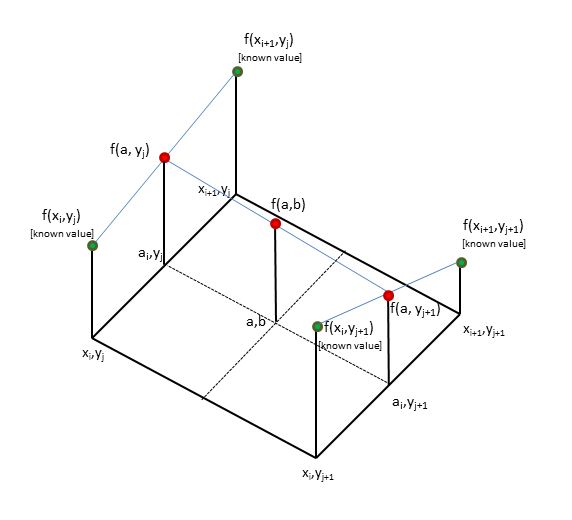
\includegraphics[width=0.7\textwidth]{interpolacion_bilineal.png}
    %
    \caption{Interpolación bilineal\protect\footnotemark}\label{fig:interp_bilineal}
    % \footnote{A}}
\end{figure}

\footnotetext{\url{https://stackoverflow.com/questions/8808996/bilinear-interpolation-to-enlarge-bitmap-images}}

Si bien hay otros métodos de interpolación para estimar el valor de $C_D$ a
partir de una nube de puntos, este método es sencillo y da resultados
satisfactorios.
%
En la Figura~\ref{fig:bilineal} se muestra a modo de ejemplo del error obtenido
con este método para interpolar una función de prueba
$f=\sin\left(\sqrt(x^2 + y^2)\right)$.

\begin{figure}
    \centering
    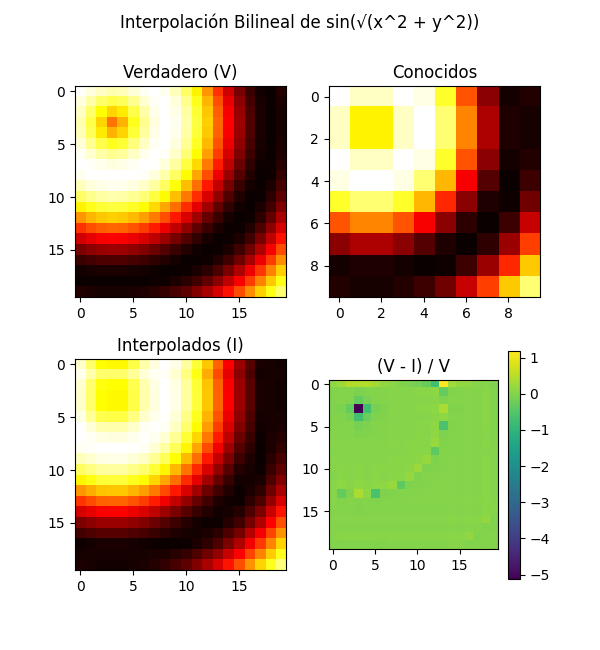
\includegraphics[width=0.7\textwidth]{bilineal.png}
    \caption{Interpolación bilineal de $\sin(\sqrt(x^2 + y^2))$}\label{fig:bilineal}
\end{figure}

La malla rectangular requerida para la interpolación bilineal del mapa de
$C_{D}$ se realizará a partir de los valores resultantes de las flujometrías con
\emph{OpenFOAM}~\parencite{openfoam}.
%
Debido al costo computacional que requieren las flujometrías, solo una cantidad
reducida de puntos se obtendrá con este método.
%
Se tiene como punto de partida una malla no rectangular, por lo que se utiliza
un método intermedio para obtener una matriz de puntos que pueda ser leída por
la interpolación bilineal.

Se probaron dos métodos para realizar la interpolación, el método del punto más
cercano (MC) y la interpolación por la suma de la inversa de la distancia o IDW por
sus siglas en inglés (\emph{Inverse Distance Weighting}).
%
Estos se combinan con métodos de suavizado de promedio móvil con los $S$ valores
más cercanos, con este método cada valor original de la matriz se reemplaza por
el promedio aritmético de los valores a $S$ filas o columnas de distancia.
%
En la Figura~\ref{fig:suavizado_promedio} se muestra este proceso para una
matriz $5\times5$.

\begin{figure}
    \centering
    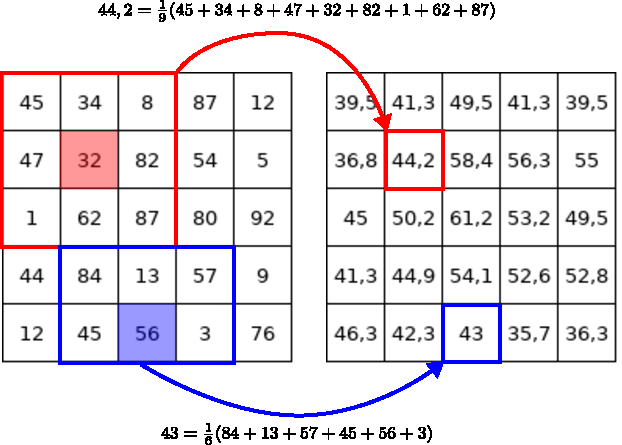
\includegraphics[]{/mapa_cd/suavizado.pdf}
    \caption{Suavizado por promedio con celdas vecinas, S=1}\label{fig:suavizado_promedio}
\end{figure}


El método del punto más cercano consiste en asignar para cada par $(x, y)$ el
valor conocido más cercano, ver Algoritmo~\ref{algo:mas_cercano}.

\begin{algorithm}
 \caption{Interpolación por punto más cercano}\label{algo:mas_cercano}
    \KwIn{\\
        $V_x, V_y$: valores de $x, y$ en los que se conoce el valor en $z$.\\
        $V_z$: valores conocidos de $z$.\\
        $I_x$: $n$ puntos de $x$ donde se quiere interpolar\\
        $i_y$: $m$ puntos de $y$ donde se quiere interpolar\\
        }

    \KwResult{Devuelve una matriz $I_{[n,m]}$ con los valores interpolados,
      donde a cada punto $I(x,y)$ se le asigna al valor de $v_z$ más cercano
      conocido. Da como resultado superficies escalonadas.}

    \BlankLine
     $I=zeros_{[n,m]}$\;
     \For{$i \gets 0$\KwTo$n$}{
        \For{$j \gets 0$\KwTo$m$}{
          $d = \sqrt{{(V_x - I_{xi})}^2 + {(V_y - I_{yj})}^2}$\;
            $I[i,j] = v_z[\min(d)]$\;
        }
     }
\end{algorithm}

La interpolación por IDW consiste en asignar a cada punto el resultado de un
promedio de los valores cercanos, ponderado por la distancia elevado a un
exponente arbitrario $p$.
%
Cuanto más grande el valor de $p$, más sensible es el método a los valores
cercanos.
%
La ecuación del promedio es la~(\ref{eq:idw}) y en el Algoritmo~\ref{algo:IDW}
se presenta el esquema utilizado.
%
En la Figura~\ref{fig:mapas_interpolados} se muestra una comparación de ambos
métodos, para una malla de $C_{D}=f(\Delta_{P}, l_{v})$ generada al azar.

\begin{equation} \label{eq:idw}
    f_p = \frac{\sum_{i=1}^{n} \frac{z_i}{d_i^p}} {\sum_{i=1}^{n}
    \frac{1}{d_i^p}}
\end{equation}

\begin{algorithm}
    \caption{Interpolación IDW}\label{algo:IDW}
    \KwIn{\\
        $V_x, V_y$: valores de $x, y$ en los que se conoce el valor en $z$.\\
        $V_z$: valores conocidos de $z$.\\
        $I_x$: $n$ puntos de $x$ donde se quiere interpolar\\
        $i_y$: $m$ puntos de $y$ donde se quiere interpolar\\
        $p$: potencia a la que se eleva cada peso\\
        }

    \KwResult{Interpolación ponderada por inverso de la distancia. Dependiendo
      del valor de $p$, se obtienen valores más o menos suavizados.}

    \BlankLine
    $I=zeros_{[n,m]}$\;
    \For{$i \gets 0$\KwTo$n$}{
        \For{$j$\gets 0 \KwTo$m$}{
          $d = {\left[{(V_x - I_{xi})}^2 +{(V_y - I_{yj})}^2\right]}^{\frac{p}{2}}$\;
          \eIf{$\exists i : d[i] = 0$}{
            $I[i, j] = V_z[i]$\;
          }{
            $I[i,j] = \frac{\sum{V_{zi}/d_i}}{\sum \frac{1}{d}}$\;
          }
        }
     }
\end{algorithm}


\begin{figure}
    \centering
    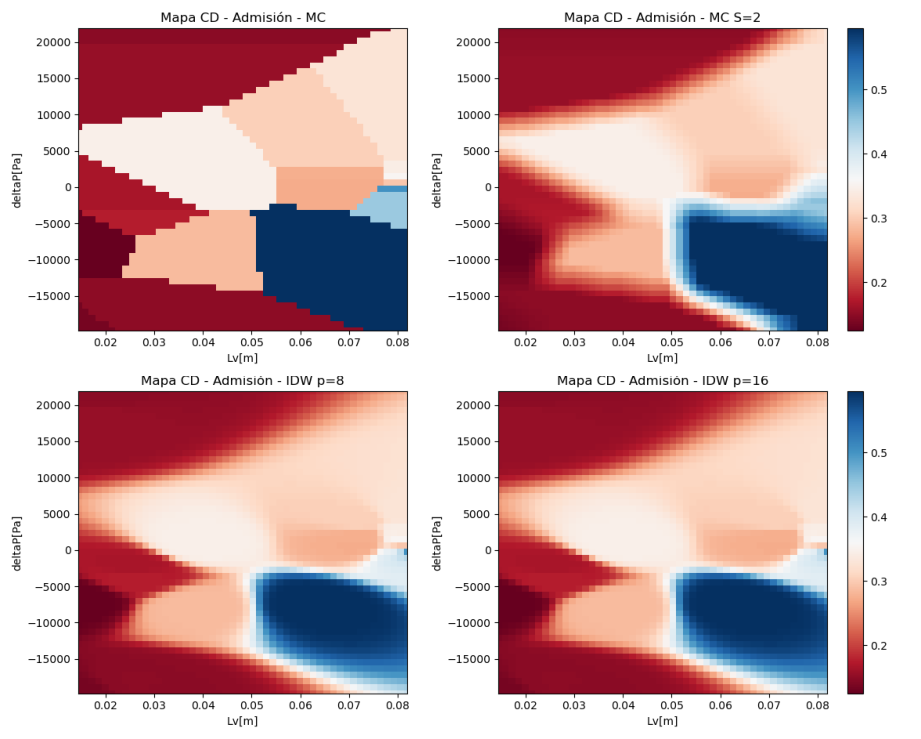
\includegraphics[width=.7\textwidth]{mapa_cd/mapa_cd.pdf}
    \caption{Comparación de métodos de interpolación}\label{fig:mapas_interpolados}
\end{figure}

%%%%%%%%%%%%%%%%%%%%%%%%%%%%%%%%%%%%%%%%%%%%%%%%%%%%%%%%%%%%%%%%%%%%%%%%%%%%%%%

\subsection{Área de Referencia}
%
El área de referencia utilizada por ICESym es el área de
cortina~(\ref{eq:area_cortina}) y se expresa en el código del programa como el
área efectiva $F_{V}=A_{R}\cdot C_{D}$.
%
Como se indicó en el apartado~\ref{sec:cap2_cd}, para el  MRCVC el área de
referencia es el área frontal del puerto expuesta a la cámara, calculada como la
altura de la ranura $h_{p}$ multiplicada por la distancia entre el borde del
puerto y la paleta que delimita la cámara, denominada como $l_{v}$.

%
% En la Figura~\ref{fig:area_referencia} se ilustran las áreas de referencia para
% una posición del rotor en la que hay solape de cámaras con $\theta = 55^\circ$.
%
Este valor se afecta por el coeficiente de descarga intermedio $C_{D,int}$, que
puede ser un valor fijo o el resultado de interpolar de un mapa de $C_D$ para un
valor de cuerda y $\Delta_P$ dado, como se indica en la ecuación~(\ref{eq:fv}).

\begin{equation}\label{eq:fv}
    F_v = C_{D,int}\cdot h_{p}\cdot l_{v} = 0,0294\cdot C_{D,int}\cdot l_{v}
\end{equation}

% \begin{figure}
%     \centering
%     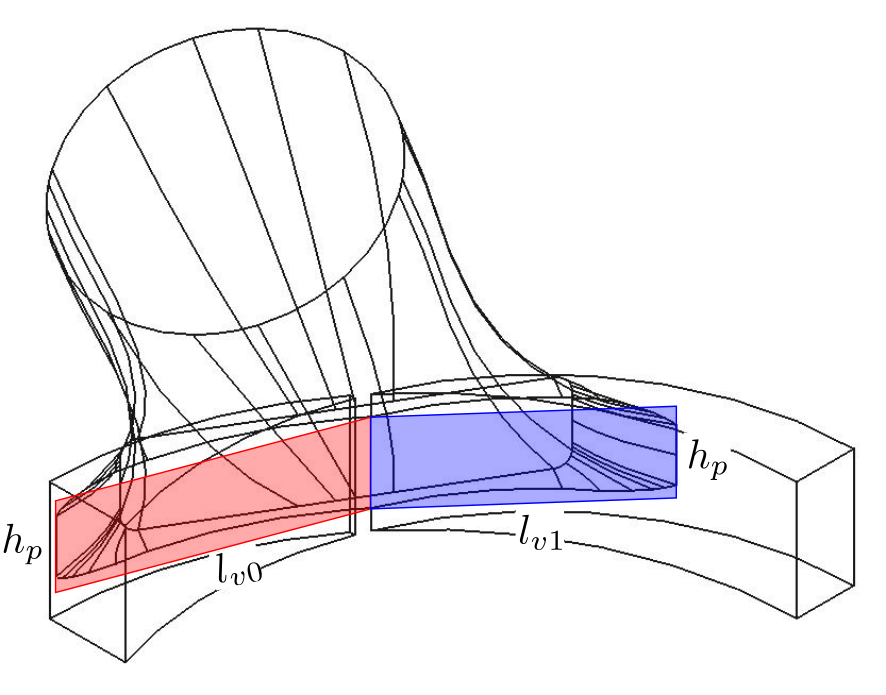
\includegraphics[]{area_referencia.png}
%     \caption{Área de referencia}\label{fig:area_referencia}
% \end{figure}

Tanto al inicio como al cierre del puerto ocurre solape de cámaras, por lo que
en estos intervalos angulares hay un valor de $C_D$ para cada cámara.
%
Este se calcula con el flujo másico que atraviesa las secciones de entrada
correspondientes a cada cámara y el área de puerto expuesta por cada cámara.

\subsection{Interfaz con Optimizador}
%
Para lograr ejecutar el simulador automáticamente, se creó una librería de
funciones capaz de tomar como dato de entrada un archivo de configuración que
incluye geometría, velocidades a ejecutar y cantidad de ciclos de simulación,
entre otros.

Para ejecutar una instancia de ICESym se puede utilizar la interfaz gráfica de
usuario (GUI) ó ejecutarlo por línea de comando desde una consola.
%
El simulador de motores se ejecuta como un archivo de Python {\tt>> python
main.py}, elc ual archivo contiene las instrucciones que lanzan la simulación del
motor con una configuración dada.
%

ICESym requiere de un archivo de configuración con los datos de la simulación a
realizar, este archivo se organiza como sigue:

\begin{forest}
  [config.py
    [Atmospheres]
    [Junctions]
    [Simulator]
    [Cylinders
      [Combustion]
      [Fuel]
      [Inyection]
      [Valves]]
    [Tanks]
    [Tubes]
  ]
\end{forest}

\begin{itemize}
  \item {\tt Atmospheres}: contiene el estado de la atmósfera, que es condición de
contorno de la simulación: presión, densidad y velocidad inicial.
  \item {\tt Cylinders}: geometría y condiciones de contorno, estado inicial,
combustible, como así también de las válvulas.
  \item {\tt Valves}: geometría, tipo de válvula, modelo de $C_{D}$, perfil de alzada y
datos de $C_{D}$ y tubo conexionado.
  \item {\tt Junctions}: contiene información de las uniones entre tubos.
  \item {\tt Simulator}: configuración de la simulación, velocidades a simular,
propiedades de gas, combustible, directorios, entre otros.
  \item {\tt Tanks}: volumen, masa y temperatura de pared de tanques.
  \item {\tt Tubes}: geometría, cantidad de nodos y conexiones.
\end{itemize}

Los elementos de configuración intervenidos por el optimizador son {\tt
Cylinders}, {\tt Valves} y {\tt Simulator}; donde se pueden modificar según
necesidad los siguientes valores:

\begin{itemize}
  \item {\tt Simulator}:
        \begin{itemize}
          \item {\tt RPMS}: Velocidades a simular (por ejemplo una lista de [1000,
2000, \ldots, 9000).
          \item {\tt NCYCLES}: cantidad de ciclos por velocidad (un entero mayor o igual a 1).
          \item {\tt FOLDER NAME}: nombre de la carpeta donde se guardan los
resultados de la simulación.
          \item {\tt SHOW INFO}: selector para mostrar o no información de la simulación.
          \item {\tt CONFIG DATA}: archivo donde se guarda la configuración utilizada.
        \end{itemize}
  \item {\tt Cylinders} $\longrightarrow$ Valves
        \begin{itemize}
          \item {\tt LvI}: perfil de alzada del puerto de admisión.
          \item {\tt LvE}: perfil de alzada del puerto de escape.
          \item {\tt IPO}: ángulo de apertura del puerto de admisión.
          \item {\tt IPC}: ángulo de cierre del puerto de admisión.
          \item {\tt EPO}: ángulo de apertura del puerto de escape.
          \item {\tt EPC}: ángulo de cierre del puerto de escape.
          \item {\tt cd\_model}: selector de modelo de $C_{D}$.
                \begin{itemize}
                  \item $C_{D}l_{v}$ valores de alzada para el mapa de $C_{D}$(
para modelo de 2 variables).
                  \item $C_{D}d_{p}$ valores de $\Delta_{P}$ para el mapa de
$C_{D}$ (para modelo de 2 variables).
                  \item $C_{D}$ valores de $C_{D}$ relacionados con alzada (para modelo de 1 variable).
                \end{itemize}
          \item $D_{v}$: diámetro de la cabeza de la válvula.
        \end{itemize}
  \item Tubes
        \begin{itemize}
          \item longitud: longitud total del tubo de admisión o escape.
        \end{itemize}
\end{itemize}
 \label{capitulo:3_icesym} \pagebreak
\section{Optimizador y Algoritmo Genético}
%
% Se seleccionó un algoritmo genético (AG) como método de optimización por ser un
% método sencillo de programar además, este tipo de algorimto es de utilidad
% cuando se tiene una solución con uno o más máximos óptimos locales ó cuando no
% se tiene certeza sobra la suavidad de la función a evaluar.
%

Se seleccionó un algoritmo genético (AG) para realizar la optimización de la
geometría del MRCVC por la simplicidad y facilidad de implementación del mismo.
%
Si bien este tipo de métodos no garantiza que se alcance un resultado óptimo,
en la práctica se ha observado que alcanzan soluciones muy cercanas a las
óptimas tras pocas iteraciones del método~\parencite{goldberg}\parencite{shi}.

Una de las ventajas de este método es que no requiere información del gradiente
de la función que se está evaluando, lo cual es útil cuando no se puede asegurar
la existencia de la derivada de la función en todo el dominio ó cuando se tiene
una función con más de un máximo o mínimo local.
%
Además, el punto de partida de la optimización es una población generada al
azar, se tiene un muestreo aleatorio del dominio que se está evaluando.
%
Esto hace que el método sea poco susceptible a dar como resultado óptimos
locales.

Se puede decir que un algoritmo genético es un método de búsqueda aleatoria
guiada.
%
¿Cómo difieren los AG de los métodos tradicionales de búsqueda?
%
\begin{enumerate}
  \item Los AG pueden operar sobre una representación de las variables estudiadas y
no necesariamente sobre las variables de estudio.
  \item Cada iteración utiliza un conjunto de datos con cierto grado de
aleatoriedad.
  \item Utilizan una función objetivo para evaluar cada punto sin necesidad de
conocer la derivada de la función que se está evaluando.
  \item Los AG usan reglas probabilísticas de decisión.
\end{enumerate}


% \subsection{Componentes básicos de un AG}
%
Los mecanismos básicos que hacen a un algoritmo genético son: 1) SELECCIÓN, 2) CRUZA y 3) MUTACIÓN.
%
El funcionamiento básico se sintetiza en el pseudocódigo~\ref{algo:genetico}.

La SELECCIÓN consiste en crear individuos a partir del puntaje que devuelve
una función objetivo, la cual es la encargada de guiar el proceso de
optimización dando mayor o menor puntaje a un candidato según el resultado que
se quiere obtener.
%
Este paso significa que, aquellos individuos a los cuales se les asignó un
puntaje más elevado tienen más probabilidades de ser copiados o de
``transmitir'' sus parámetros a la iteración siguiente.
%
Este proceso imita en cierta forma la selección natural o evolución Darwiniana y
de aquí viene el nombre de algoritmo genético o evolutivo.

El segundo operador es la CRUZA, consistente en combinar los parámetros de dos
individuos para obtener uno nuevo, esto se asemeja a la reproducción.

Finalmente la MUTACIÓN es la encargada de modificar aleatoriamente uno o más
parámetros de cada nuevo individuo.
%
Este operador juega un rol secundario pero muy importante en la simulación, es
secundario porque se pueden alcanzar soluciones satisfactorias sin que exista la
mutación de la población.
%
Importante porque utilizado con probabilidades pequeñas de ocurrencia, permite
evitar la pérdida temprana de información relevante o convergencia temprana.
%
Por otro lado, en caso de que la probabilidad de mutación sea muy alta, el AG se
convierte en un método de búsqueda aleatoria.

\begin{algorithm} \caption{Algoritmo de optimización}\label{algo:genetico}
  Inicializar población, al azar o a partir de una población ``semilla''.\;
  %
  \While{no se cumpla condición de parada}{
    %
    SELECCIONAR a los individuos más aptos, evaluandolos según la función objetivo.\;
    %
    CRUZAR los candidatos seleccionados para crear la nueva población (la
próxima iteración del método)\;
    %
    MUTAR algunos individuos de la nueva población\;
    %
    \If{se cumple la condición de parada}{
      Parar\;
    }
  }
  {Guardar resultados\;}
\end{algorithm}

%
% \subsection{Implementación}
%
Gran parte de este trabajo consistió en implementar y utilizar a ICESym como LA
función objetivo, aprovechando la cualidad de ``caja negra'' con la que se puede
implementar el simulador.
%
Para lograr esto se modificó parte del código de ICESym con el objetivo de
facilitar la configuración, ejecución y lectura de los resultados que arroja el
simulador y así poder ejecutar de manera automática una simulación con una
configuración particular del motor.
%
Otro aspecto del optimizador que se desarrolló, es el de poder ejecutar
múltiples instancias de ICESym en paralelo con el fin de reducir el tiempo de
ejecución de cada simulación, pudiendo evaluar varios motores (o individuos) al
mismo tiempo.

Para la primera iteración se programaron desde cero los algoritmos y funciones
necesarias para llevar a cabo la optimización con el AG.
%
Posteriormente se tomó la librería DEAP~\parencite{DEAP_JMLR2012} y se
modificaron los operadores a medida, para poder utilizarlos con ICESym.

En los apartados siguientes se describe la implementación de cada uno de los
operadores en el optimizador.

\subsection{Población}
%
Se decidió representar cada motor como un vector con las dimensiones y reglaje
que definen la geometría del sistema de intercambio de gases, los cuales se
listan en la Tabla~\ref{tab:param_motor}.
%
Se limitaron los valores que puede tomar cada parámetro para que la geometría
resultante se asemeje a la geometría del motor utilizado en trabajos anteriores,
aprovechando así los resultados obtenidos en el primer barrido paramétrico.


\begin{table}[ht]
  \centering
  \begin{tabular}{rllll} \toprule
    Nº & Parámetro & Descripción & Sistema & Límites \\ \midrule
    1 & DTA & Diámetro de tubo & Admisión & [60, 100] mm \\
    2 & DTE & Diámetro de tubo & Escape & [60, 100] mm\\
    3 & LIT & Largo de tubo & Admisión & [300, 2000] mm\\
    4 & LET & Largo de tubo & Escape & [300, 2000] mm\\
    5 & IIA & Ángulo geométrico de apertura & Admisión & [0,90]º \\
    6 & IFA & Ángulo geométrico de cierre & Admisión & [IIA, 90]º \\
    7 & IIE & Ángulo geométrico de apertura & Escape & [0, 90]º \\
    8 & IFE & Ángulo geométrico de cierre & Escape & [IIA, 90]º \\ \bottomrule
  \end{tabular}
  \caption{Parámetros que representan al motor}\label{tab:param_motor}
\end{table}


Se decidió representar los vectores que hacen a cada motor como un número
binario de 40 dígitos, ocupando 5 dígitos para representar cada uno de los 8
parámetros que hacen a cada motor.
%
Esto facilita la implementación de los operadores de selección, cruza y
mutación, pudiendo aprovechar implementaciones de operadores existentes en
librerías como DEAP.
%
Estos 8 números binarios luego se convierten una lista de enteros mediante una
transformación lineal $f(x)=a\cdot x+b$, en la que se ingresa con un entero
entre 0 y $2^{n}-1$ para ir del número binario a un decimal, siendo $n$ la
cantidad de dígitos del binario (en este caso 5).
%
Los coeficientes $a$ y $b$ son tales que $f(0)=x_{0}$ y $f(2^{n}-1) = x_{1}$,
donde $x_{0}$ y $x_{1}$ son los extremos del rango para el que se quiere aplicar
la transformación.
%
Estos coeficientes ($a$ y $b$) son particulares a cada parámetro, porque se
determinan de acuerdo a los valores que puede tomar cada uno.

De este modo se obtiene el valor de cada uno de los parámetros que hacen a la
configuración particular de cada motor en ICESym.
%
El orden de los mismos se mantiene constante, por lo que cada sección del número
representa una característica en particular del motor, como se muestra en el
ejemplo de la Figura~\ref{fig:pop_bit}.
%

\begin{figure}[ht]
  \centering
  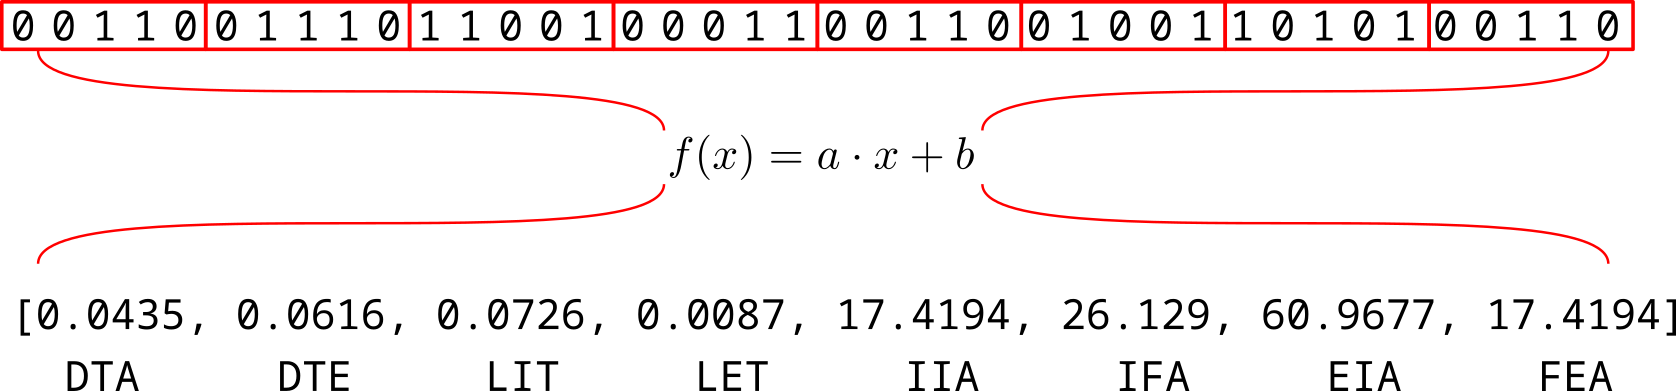
\includegraphics[]{genetico/representacion_bits.png}
  \caption{Representación del individuo}\label{fig:pop_bit}
\end{figure}


\subsection{Reproducción}

Para crear la nueva población se debe elegir a los nuevos candidatos basándose
en los puntajes de la población actual.
%
Hay varios métodos diferentes de selección, como son de ruleta, aleatoria, por
puntaje y de tipo torneo.
%
Para este trabajo se seleccionó el método de torneo, que consiste en comparar
los puntajes de $n$ individuos seleccionados al azar y el que tenga el mejor
puntaje es el seleccioando o ganador.
%
La cantidad de individuos comparados $n$ es el tamaño de muestreo o de torneo,
cuanto más grande sea este número más posibilidades tienen de ganar los
individuos con mayor puntaje, y la cantidad de rondas del torneo determina la
cantidad de individuos seleccionados para participar en la próxima iteración o
generación de candidatos.


\subsection{Cruza}
%
El operador de cruza se encarga de combinar los genes de dos individuos para
producir un individuo nuevo; la función es la de intercambiar los parámetros que
hacen a uno y otro para dar lugar a una nueva posible solución.
%
Para individuos representados por un vector se suelen usar operadores de tipo
cruza de uno o múltiples puntos como también cruza uniforme.
%
El método seleccionado es \emph{cruza de dos puntos}, en este método
se corta el vector que forma al individuo en dos puntos, la posición de estos
puntos se selecciona al azar, manteniendo el largo original de los vectores.
%
Luego los individuos ``cruzados'' se combinan de forma complementaria, como se muestra
la Figura~\ref{fig:cr2puntos}.
%
En el algoritmo~\ref{algo:cr2puntos} se esquematiza
el proceso.
%
% TODO: pongo pseudocódigo? o dejo el còdigo

\begin{figure}[ht!]
  \centering
  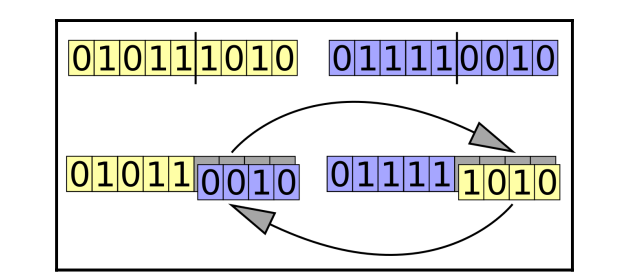
\includegraphics[width=0.5\textwidth]{cruza2puntos.png}
  \caption{Cruza de dos puntos}\label{fig:cr2puntos}
\end{figure}


\begin{algorithm}[]
  \KwIn{\\
    $ind_{1}, ind_{2}$: dos individuos de entrada [101\ldots011], [110\ldots100]\\
    EA(a, b): devuelve un Entero al Azar entre los enteros a y b.\\
    L(a): devuelve la cantidad de elementos en a.}
  \KwOut{\\
    $ind_{1}, ind_{2}$: individuos de entrada modificados}
  \SetKwFunction{EA}{EA}
  \SetKwFunction{L}{L}
  % \SetKwFunction{min}{min}
  \BlankLine
  s = min(\L{$ind_{1}$}, \L {$ind_{2}$})\;
  $CX_{1} = \EA{1, s}$\;
  $CX_{2} = \EA{1, s-1}$\;
  \eIf{$CX_{1} \geq CX_{2}$}{
    $CX_{2} = CX_{2}+1$\;
  }{
    $aux=CX_{1}$\;
    $CX_{1}=CX_{2}$\;
    $CX_{2}=aux$\;
  }
  $aux = ind_{1}$\;
  $ind_{1}[CX_{1}:CX_{2}] = ind_{2}[CX_{1}:CX_{2}]$\;
  $ind_{2}[CX_{1}:CX_{2}] = aux[CX_{1}:CX_{2}]$\;
  \Return{$ind_{1}, ind_{2}$}\;
  Terminar el programa;
  \caption{Cruza de dos puntos}\label{algo:cr2puntos}
\end{algorithm}

\subsection{Mutación}
%
La mutación juega un rol secundario pero importante, una pequeña probabilidad
de que alguno de los genes se modifique en un valor aleatorio contribuye a que
el algoritmo genético no se estanque en soluciones de máximos o mínimos locales.

Algunos de los métodos de mutación utilizados son:

\begin{enumerate}
  \item FLIP BIT
  \item INTERCAMBIO,
  \item INVERSION
  \item REORDENADO ALEATORIO
\end{enumerate}

% FLIP BIT se utiliza para números binarios y el método consiste en intercambiar
% ceros y unos con una probabilidad al azar en ubicaciones al azar, por ejemplo
% $10101 \rightarrow 11101$.

En este trabajo se utiliza el método de reordenado aleatorio en el cual se
modifica al azar el orden de los números que hacen al individuo, modificando los
índices de la lista que define el arreglo, por ejemplo:
$12345 \rightarrow 12543$.

\subsection{Función Objetivo}\label{sec:funcion_objetivo}
%
La función objetivo es la encargada de dar puntaje a los individuos, en la
analogía con la selección natural esta función es el ambiente.
%
Determina la aptitud de un motor con respecto a otro en lo que respecta a
\emph{performance} del sistema de intercambio de gases.
%
Inicialmente se propuso que la función objetivo sea la suma de los rendimientos
volumétricos a todas las velocidades simuladas $s=\sum \eta_{v}$.
%
Este tipo de funciones dió como resultado una curva de $\eta_{v}$ aserrada como
se muestra en la Figura~\ref{fig:curva_aserrada}.

\begin{figure}[ht]
  \centering
  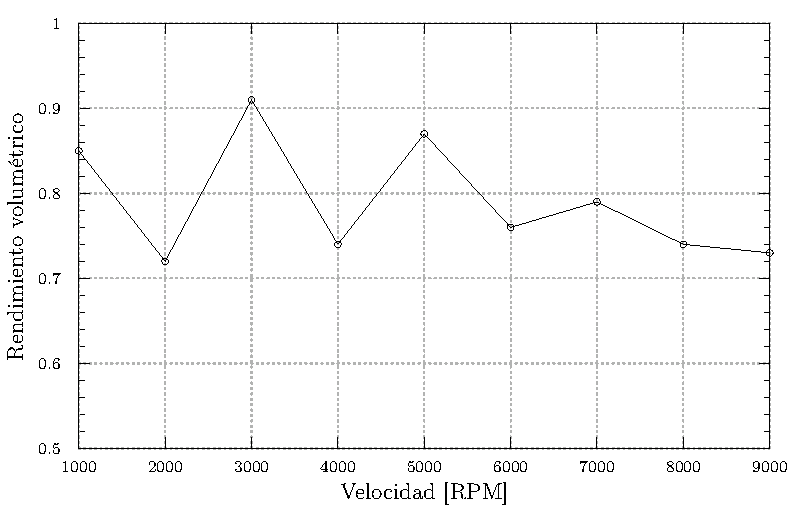
\includegraphics[width=0.7\textwidth]{gnuplot/rendimiento_aserrado.pdf}
  \caption{Curvas de rendimiento volumétrico aserradas}\label{fig:curva_aserrada}
\end{figure}

Esta curva aserrada es poco deseable porque significa una entrega de torque y
potencia dispar, por este motivo se modificó la función objetivo para favorecer
curvas suaves y preferentemente con un solo punto de inflexión.
%
Se implementó una suma ponderada para obtener un rendimiento volumétrico máximo
en un valor cercano a 6000 RPM de modo de aprovechar las características de
balanceo de fuerzas y mayores velocidades de giro de los motores rotativos.
%
La aptitud resulta de la suma del rendimiento volumétrico y el inverso de la
fracción de gases residuales, lo cual probó ser la función objetivo que mejores
resultados dió, la metodología utilizada se resume a continuación.

\begin{enumerate}
        \item Se evalúa cada motor, calculando el rendimiento volumétrico
$\eta_{v}$ y fracción de gases residuales $x_{r}$ para cada velocidad de giro
simulada.
        \item Con $\eta_{v} = (\eta_{v,1}, \ldots ,\eta_{v,n})$ y
$x_{r}=(x_{r,1},\ldots,x_{r,n})$ se hace una suma para cada velocidad
$S_{i}=\eta_{v,i} + x_{r,i}^{-1}$.
        \item Cada motor tiene un vector o lista de valores
$S = (S_{1},\ldots,S_{n})$ para cada velocidad evaluada, con la cual se calcula
el puntaje del motor como:
        \begin{equation}
        f = \sum_{i=1}^{n}{S_{i}} + S_{k}^{2}
      \end{equation}

El valor $S_{k}$ es el puntaje para la $k$-\textit{ésima} velocidad de giro (6000 RPM en
este caso) y se eleva al cuadrado para favorecer altos rendimientos en esta
velocidad.
\end{enumerate}


Durante las primeras iteraciones del método hay una gran cantidad de geometrías
inválidas que devuelven puntaje muy bajo o nulo.
%
En caso de que alguna de las soluciones tenga un puntaje relativamente alto,
existe la posibilidad de una dominancia temprana de la población, provocando
una convergencia temprana de la optimización.
%
Estos candidatos tienen una mayor probabilidad de ``pasar'' sus características
geométricas a las iteraciones siguientes y es algo especialmente problemático en
optimizaciones con poblaciones de alrededor de 100 individuos.

Para reducir la posibilidad de una convergencia temprana se utiliza un método de
escalado de puntajes, que consiste en una transfomración lineal en la que se
define el puntaje bruto de un individuo como $f$ y el puntaje escalado como
$f'$, la relación entre ambos es $f' = a\cdot f + b$.
%
Los coeficientes $a$ y $b$ se determinan de modo que $f'_{media}=f_{media}$, de
este modo un motor con puntaje promedio tiene la misma influencia sobre la
población ya sea con la aptitud original o escalada.
%
Para controlar la influencia del mejor individuo de una generación sobre la
próxima, los puntajes se transforman de tal modo que
$f'_{max}=C_{mult}f_{media}$.
%
El valor de $C_{mult}$ es la cantidad de copias que se espera obtener del mejor
de los candidatos en la generación siguiente y se usa en $1,2$ a $2$ para
poblaciones de entre 50 y 100 individuos~\parencite{goldberg}.

Hacia el final donde la diferencia entre puntajes de los individuos de la
población tiende a achicarse, el parámetro $C_{mult}$ cumple la función de
acrecentar las diferencias entre individuos.

En caso de existir individuos con puntaje muy bajo o nulo se hace un
pre-escalado del puntaje que fija el mínimo en $f'_{min}=0$.
%
El procedimiento se lista en los algorimtos \ref{algo:pre-escala} y
\ref{algo:pop_scale}.


\begin{algorithm} \caption{Algoritmo de pre-escalado}\label{algo:pre-escala}
  \KwIn{\\
    $F$, es un vector que contiene los puntajes de todos los individuos\;\\
    $C_{mult}$, es un multiplicador para el escalado, se suele usar
$f\in[1.2, 2]$\;\\ }
  \KwOut{\\
    $a, b$, son los coeficientes para la transformación lineal $f(x)=a\cdot x + b$\;
  }
  \SetKwFunction{max}{max}
  \SetKwFunction{min}{min}
  \SetKwFunction{media}{media}
  \BlankLine

  $u_{max} = \max{F}$\;
  $u_{min} = \min{F}$\;
  $u_{medio} = \media{F}$\;
  \eIf{$u_{min}> aux = (C_{mult}\cdot u_{medio} - u_{max}) \mathbin{/} (C_{mult}-1)$
    }{
    $\Delta_{u} = u_{max}-u_{avg}$\;
    $a = (C_{mult} - 1) \cdot u_{avg} / \Delta u$\;
    $b = u_{avg} \cdot (u_{max} - C_{mult} \cdot u_{avg}) \Delta_{u} $\;
  }{
    \eIf{$\Delta \neq 0$}{
      $a = u_{avg} \mathbin{/} \Delta_{u}$\;
      $b = -u_{min} \cdot u_{avg} \mathbin{/} \Delta_{u}$ \;
    }{
      $a=1$\;
      $b=0$\;
    }
  }
  \Return{$a, b$}
\end{algorithm}


\begin{algorithm}\caption{Escalado de población}\label{algo:pop_scale}
  \KwIn{\\
    $f$, es la aptitud.\\
    $a, b$, son los parámetros de la función de pre-escalado. \\
  }
  \KwOut{\\
  $f^{*}$, los puntajes escalados.}
  \SetKwFunction{ps}{PreEscalado}
  \SetKwFunction{ll}{Largo}
  \SetKwFunction{esc}{Escala}
  \BlankLine

  $a, b = \ps{f, 2}$\;
  $f^{*} = ()$ \;
  $n = \ll{f}$\;
  \For{$i=1$ \KwTo $n$}{
    $f^{*}_{i} = a\cdot f_{i} + b$\;
  }
  \Return{$f^{*}$}\;
\end{algorithm}

% Con la población definida se procede a los evaluar cada motor con la función
% objetivo, la cual se definió de manera tal de favorecer curvas de rendimiento
% volumétrico suaves y valores altos a mayores RPM.\@

% La suavidad de la curva de rendimiento volumétrico se calcula midiendo los
% cambios de pendiente de la derivada la cual se aproxima con la fórmula de
% diferencia progresiva~\ref{eq:derivada}.
% %
% Solamente interesa el signo, por lo que el valor de $h$ en el denominador no
% interesa y se hace 1, con esto la función objetivo queda como el
% algoritmo~\ref{alg:funcObj}.

% \begin{equation}\label{eq:derivada}
%   f' = \frac{f(i+1) - u(i)}{h}
% \end{equation}

% Una vez evaluados todos los motores de la población, se debe seleccionar los
% individuos que formarán la siguiente iteración del algoritmo.
% %
% El método de selección es de tipo TORNEO, en el cual se seleccionan los mejores
% $k$ individuos de un grupo al azar de $N$ candidatos.
% %

% Con los nuevos candidatos seleccionados, se procede a variar la población,
% realizando la cruza y mutación.

% Luego se toman pares de individuos y de acuerdo a la probabilidad de cruza, se
% combinan con el método seleccionado.

% Finalmente se realiza una segunda iteración sobre la nueva población, aplicando
% el método de mutación a cada individuo, de acuerdo a la probabilidad de
% mutación indicada.
%
 \label{capitulo:3_optimizador} \pagebreak
\section{OpenFOAM}\label{sec:3_openfoam}
%
Las flujometrías se realizaron con \emph{OpenFOAM}, un software de
Fluidodinámica Computacional, o CFD por sus siglas en inglés, de código libre y
abierto escrito en ``C++''.
%
% La herramienta seleccionada para realizar las flujometrías es OpenFOAM, por ser
% una herramienta libre y de código abierto.
%
Junto con este programa se utilizaron otras herramientas libres para generar la
geometría a modelar y post-procesar los resultados..
%
El esquema de trabajo para realizar las simulaciones consistió en:

\begin{enumerate}
        %
    \item Pre-procesado
      %

        \begin{enumerate}
                %
            \item Definir la geometría a analizar.
              %
            \item Generar una malla con un tamaño de elemento adecuado (la
solución a problemas de CFD depende fuertemente de la cantidad y tamaño de
celdas utilizadas).
              %
            \item Seleccionar los modelos adecuados.
              %
            \item Definir las propiedades del fluido.
              %
            \item Definir las condiciones de borde.

              %
        \end{enumerate}
        %
    \item Solver
      %
    \begin{enumerate} \item Seleccionar el solver a utilizar.
            %
            \item Ejecutar la simulación.
            %
    \end{enumerate}
        %
\item Post-procesado
      %
    \begin{enumerate}
                %
        \item Visualizar los resultados de las distintas variables de la
            simulación.
            %
        \item Extraer la información necesaria.
            %
    \end{enumerate}
        %
\end{enumerate}

%%%%%%%%%%%%%%%%%%%%%%%%%%%%%%%%%%%%%%%%%%%%%%%%%%%%%%%%%%%%%%%%%%%%%%%%%%%%%%%

\subsection{Pre-procesado}
%
El preprocesado consiste en definir geometría y condiciones iniciales de la
simulación a partir de los datos obtenidos de las simulaciones con el
optimizador e ICESym.
%
Con los resultados del simulador se grafica la diferencia de presión entre el
puerto de admisión o escape y la cámara correspondiente en función de la apertura
del puerto, para un rango de velocidades de 1000 a 9000 RPM, con el fin de
identificar las zonas en las condiciones operativas en las que evaluar el puerto.
%
En la Figura~\ref{fig:puntos_interes} se muestra una gráfica de $\Delta P$ y
alzada para los puertos de admisión y escape de 1000 a 2000 RPM de un motor
resultante de una de las simulaciones.

Como es de esperarse se tienen mayores diferenciales de presión a menores
aperturas del puerto porque se está próximo a los eventos de apertura o cierre
del mismo.
%
A diferencia del puerto de admisión, en el puerto de escape se ve una banda
bastante definida de operación que se hace más ``llena'' a medida que aumenta la
apertura del puerto.
%
Durante la apertura del puerto se ven las mayores diferencias de presión en las
que hay dos bandas bien definidas.
%
Se toman algunos puntos arriba en la zona con mayor $\Delta P$ y una cantidad
menor para velocidades con $\Delta P \simeq 0$.
%
A medida que el puerto se abre la diferencia de presión con el gas en la cámara
disminuye y esta banda se afina.

\begin{figure}
    \centering
    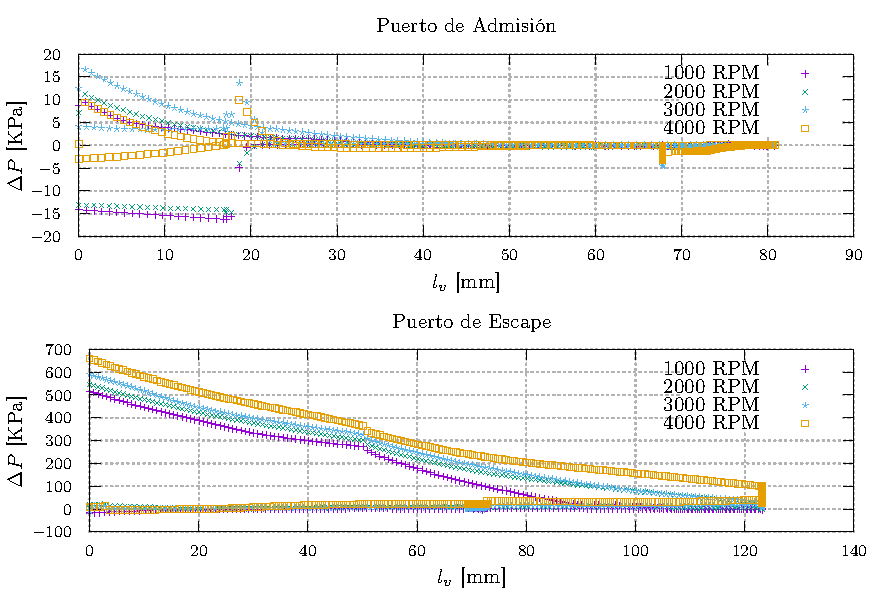
\includegraphics[width=\textwidth]{gnuplot/puntos_interes.pdf}
    \caption{Presión en función de la apertura el puerto,
$\Delta P = f(l_{v})$}\label{fig:puntos_interes}
\end{figure}

El valor de alzada está directamente relacionado con la posición angular del
cigüeñal, por lo que una vez seleccionados los puntos de interés se puede
extraer la geometría deseada de un modelo de CAD paramétrico del motor.
%
En este modelo se representó la mitad de la geometría que contiene los puertos
de admisión y escape, y se obtuvo realizando operaciones geométricas con los
volúmenes que representan diferentes componentes del motor como son el estator,
rotor, paletas, etc.
%
% En la Figura~\ref{fig:admision_50} se muestra parte del proceso para obtener el
% puerto de admisión a $\theta=50^{\circ}$, en donde se suma el volumen del mismo
% en gris y las Figuras que se restan que corresponden al rotor, las paletas y un
% paralelogramo para quitar una región que no se simuló.

\begin{figure}
    \centering
    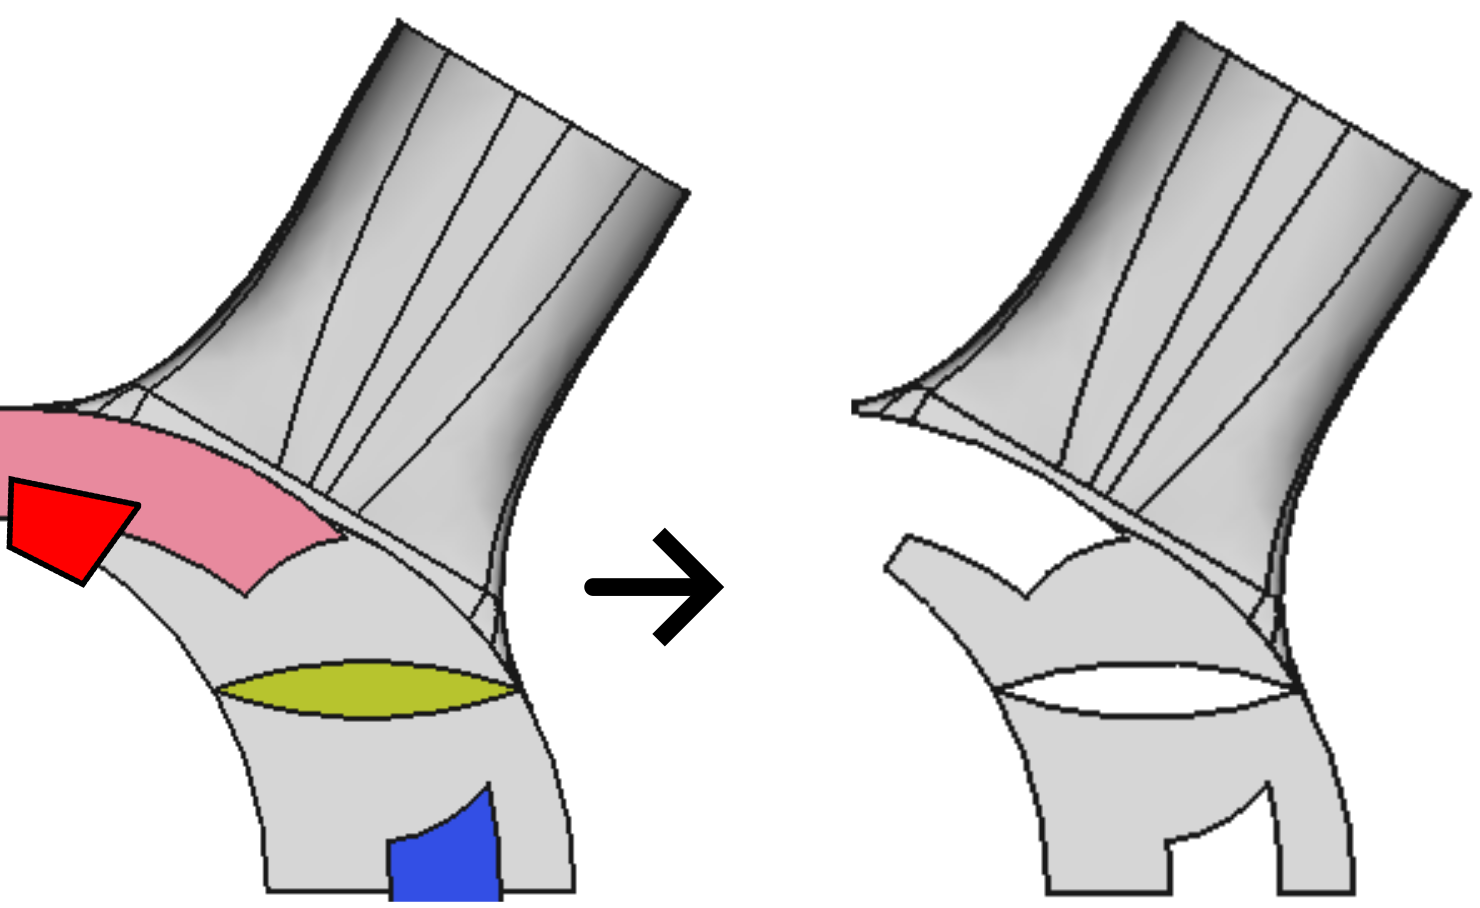
\includegraphics[width=0.7\textwidth]{./CAD/freecad_pasos.png}
    \caption{Puerto de admisión para $\theta=50^{\circ}$ modelado con
FreeCAD}\label{fig:admision_50}
\end{figure}

Esta geometría fue generada por el programa FreeCAD~\parencite{freecad},
exportada a un archivo
``.BREP''\footnote{\href{https://dev.opencascade.org/doc/overview/html/specification\_\_brep\_format.html}{Formato
BREP, opencascade.org}} para luego ser importada en Salome\parencite{salome},
que se utiliza para generar una malla cerrada, hermética, que puede ser
procesada por los complementos de OpenFOAM utilizados para generar la malla de
la simulación.
%
Es importante que se satisfaga la hermeticidad de la malla, lo cual significa
que los nodos en la frontera entre superficies coincidan, como se puede observar
en la Figura~\ref{fig:salome_malla_hermetica}, en la que se ven dos superficies
``walls'' y ``outlet'' y los nodos compartidos entre ambas superficies.
%

\begin{figure}[ht]
    \centering
    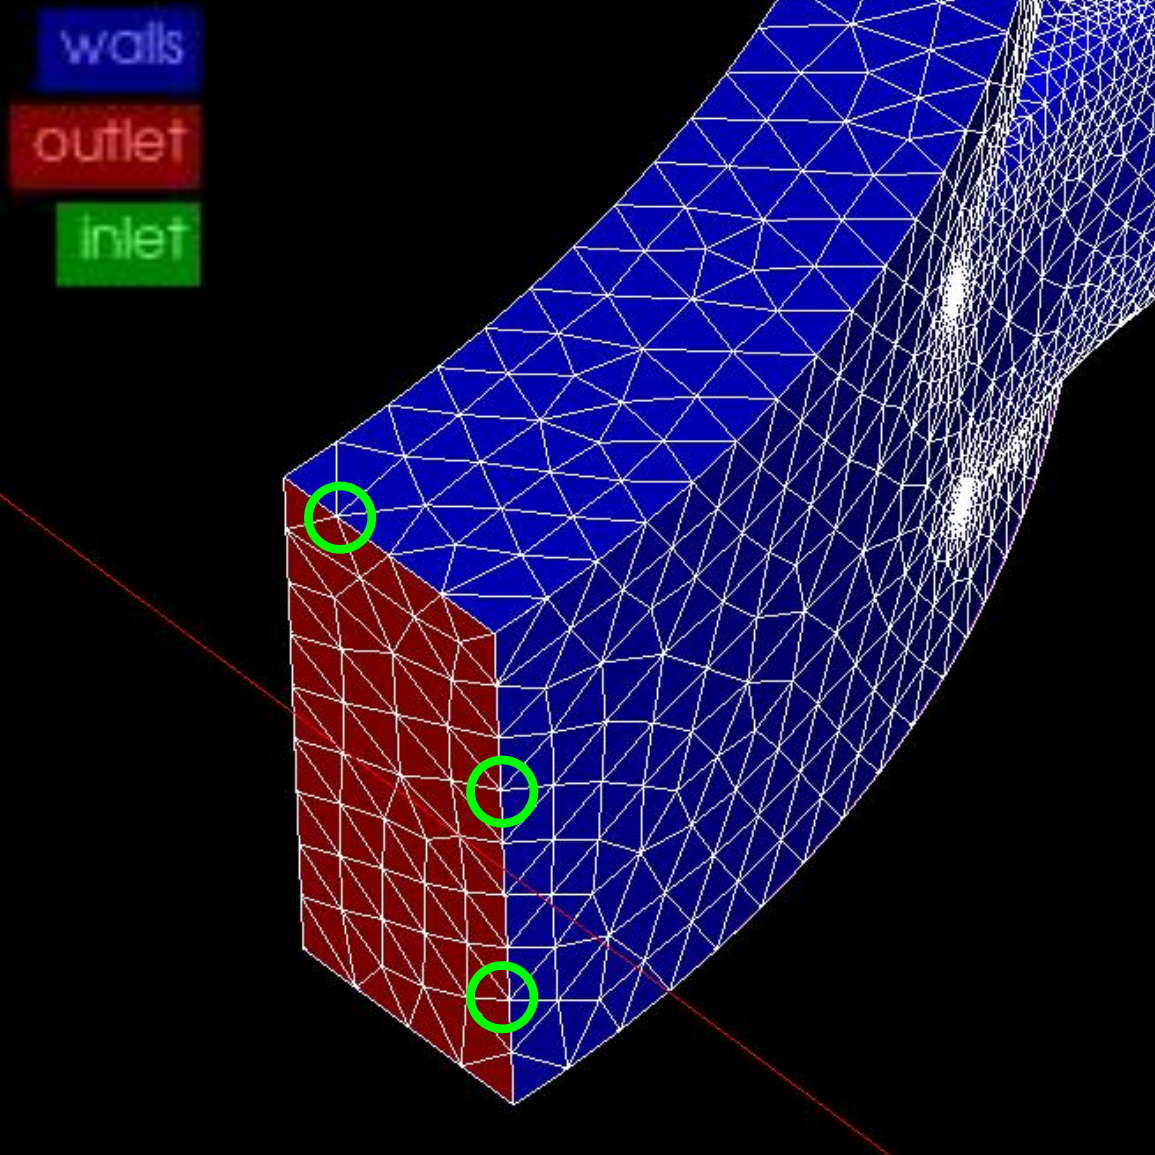
\includegraphics[width=0.4\textwidth]{./flujometrias/salome_malla_hermetica.png}
    \caption{Malla hermética}\label{fig:salome_malla_hermetica}
\end{figure}

El proceso en Salome consta de importar la geometría generada por FreeCAD y
separar la misma en superficies utilizadas para definir condiciones de contorno
en OpenFOAM.
%
Las superficies diferenciadas son: puerto, cámara/s y pared, ver
Figura~\ref{fig:openfoam_parches}.

\begin{figure}[ht]
    \centering
    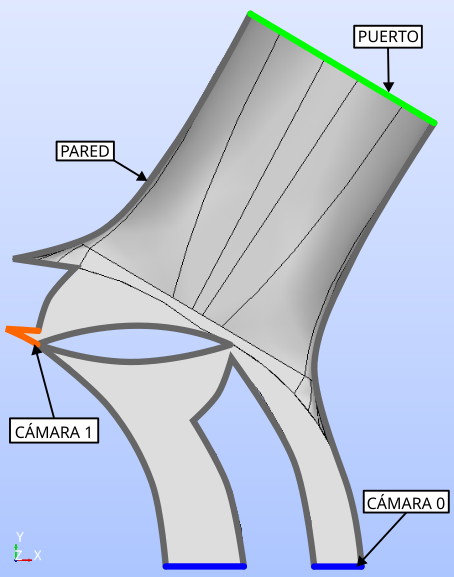
\includegraphics[width=0.5\textwidth]{./flujometrias/openfoam_parches.png}
    \caption{Nombres de Parches}\label{fig:openfoam_parches}
\end{figure}

Luego de separadas estas superficies se procede a generar la malla en formato
ASCII STL con el complemento de mallado de Salome.
%
Se utilizó el generador de mallas NETGEN 1D-2D para crear la superficie, en
general se configuró el software de modo de tener un stl de buena calidad con
elementos de menor tamaño en zonas de mayor curvatura.
%
En la Figura~\ref{fig:salome_fina_gruesa} se ve la diferencia en cantidad de
nodos de dos mallas, una malla fina a la izquierda y una malla gruesa a la
derecha.
%
En la Tabla~\ref{tab:salome_fina_gruesa} se muestra la diferencia entre algunos
parámetros básicos de configuración para las dos mallas.
%
% Esto sin requerir de una gran cantidad de elementos para no ralentizar el
% procesado con SnappyHexMesh.

\begin{figure}[t!]
    \centering
    \begin{subfigure}[t]{0.5\textwidth}
        \centering
        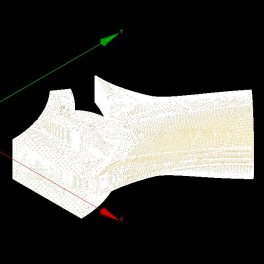
\includegraphics{/flujometrias/salome3_fina.png}
        \caption{Malla fina sin optimizar}
    \end{subfigure}%
    \begin{subfigure}[t]{0.5\textwidth}
        \centering
        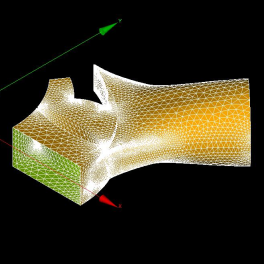
\includegraphics{/flujometrias/salome3_gruesa.png}
        \caption{Malla gruesa optimizada}
    \end{subfigure}
    \caption{Diferentes mallas para flujometrías}\label{fig:salome_fina_gruesa}
\end{figure}

\begin{table}
    \centering
    \begin{tabular}{lccc} \toprule
        Parámetro                & Malla Fina    & Malla Gruesa     & Unidades\\ \midrule
        Tamaño máximo            & 0,001         & 0,03             & m \\
        Tamaño mínimo            & 1E-7          & 2,4E-5           & m \\
        Limitado por curvatura   & Sí            & Sí               & - \\
        Optimizar                & No            & Sí               & - \\
        Cantidad de nodos        & 99311         & 49112            & - \\
        Cantidad de elementos    & 204695        & 103163           & - \\ \bottomrule
    \end{tabular}
    \caption{Configuración de mallas mostradas en la Figura~\ref{fig:salome_fina_gruesa}}
    \label{tab:salome_fina_gruesa}
\end{table}


\subsection{Configuración}
%
Para conFigurar una simulación de OpenFOAM se organiza el directorio de
simulación como se indica en la Figura~\ref{fig:direc_pf} para las flujometrías
de aire considerado como incompresible  y~\ref{fig:direc_rpf} en los casos en
los que se tiene en cuenta la compresibilidad del aire.
%
Cada directorio contiene una carpeta con condiciones iniciales ``0'', malla
``constant'', conFiguraciones particulares de cada solver ``system'' y una
caperta con los resultados del post-procesado el cual se puede realizar
durante cada paso de simulación o al final del proceso dependiendo de la
configuración que se haya utilizado.

\begin{figure}[ht!]
  \centering
  \begin{subfigure}[b]{0.4\textwidth}
    \centering
    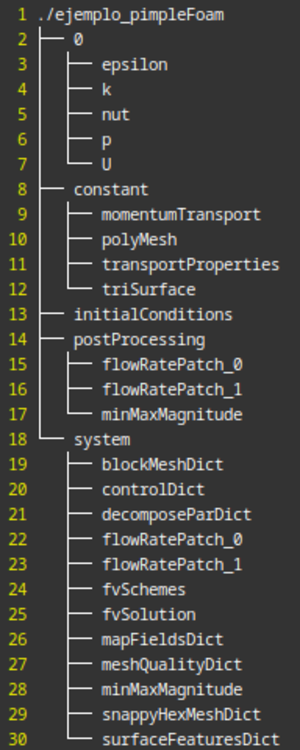
\includegraphics{flujometrias/direct_pimplefoam.pdf}
    \caption{\emph{pimpleFoam}\label{fig:direc_pf} }
  \end{subfigure}%
  \begin{subfigure}[b]{0.4\textwidth}
    \centering
    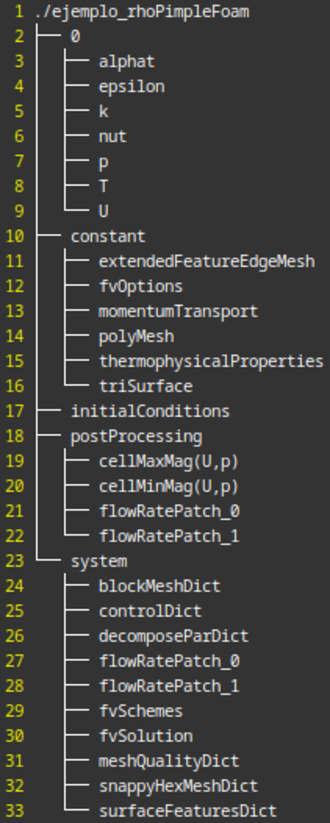
\includegraphics{flujometrias/direct_rhopimplefoam.pdf}
    \caption{\emph{rhoPimpleFoam}\label{fig:direc_rpf} }
  \end{subfigure}
  \caption{Esquema de directorios OpenFOAM}
\end{figure}


En el directorio ``0'' se indican las condiciones iniciales y de borde de cada
simulación, utilizando una configuración genérica con parámetros definidos en un
archivo separado.
%
Esto se realiza de este modo para aprovechar las características paramétricas de
OpenFOAM, permitiendo ejecutar una gran cantidad de simulaciones en serie
variando solamente los parámetros definidos en un archivo externo
``inital\_conditions.cc''.

Estos archivos de condiciones inciales se generan con un \emph{script} que toma
valores de las simulaciones de \emph{ICESym}, como se indicó en la
sección~\ref{cap2:cond_iniciales}, en la que también se detallan las ecuaciones
e hipótesis utilizadas para obtener dichos valores.
%
La ejecución de las simulaciones también se automatiza con scripts de
\emph{bash} con los pasos para ejecutar las corridas con \emph{ICESym}.
%
Con los resultados de las simulaciones se procede a calcular/leer la magnitud
del caudal másico, necesario para el cálculo del coeficiente de descarga.


\subsection{Malla}\label{sec:cap3_of_malla}
%
Una vez obtenido el archivo STL se procede a la generación de la malla dentro de
OpenFOAM con \emph{blockMesh} y \emph{snappyHexMesh}.
%
Primero se crea crea una malla con \emph{blockMesh} que  debe contener la
totalidad del volumen del puerto a simular, como se puede en la
Figura~\ref{fig:paraview_blockMesh_stl}.
%
En este paso se define el tamaño de base de la malla y el nivel general de
refinamiento.
%
A partir de estos hexaedros se produce el refinamiento por \emph{castelación}
que consiste en dividir las celdas en hexaedros más pequeños y luego aplicar el
\emph{snapping} para adaptarse a la superficie del volumen que se está
modelando, ver Figura~\ref{fig:openfoam_shm_pasos}.
%

\begin{figure}
    \centering
    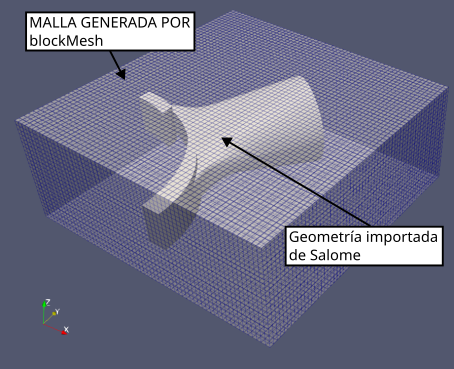
\includegraphics[width=0.5\textwidth]{flujometrias/paraview_blockMesh_stl.png}
    \caption{Malla de blockMesh y stl de Salome}\label{fig:paraview_blockMesh_stl}
\end{figure}

\begin{figure}[t!]
    \centering
    \begin{subfigure}[t]{0.5\textwidth}
        \centering
        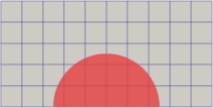
\includegraphics{flujometrias/shm_fondo.png}
        \caption{Malla de fondo y geometría}
    \end{subfigure}%
    \begin{subfigure}[t]{0.5\textwidth}
        \centering
        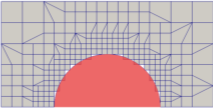
\includegraphics{flujometrias/shm_castelacion.png}
        \caption{Castelación}
    \end{subfigure}
    \begin{subfigure}[t]{0.5\textwidth}
        \centering
        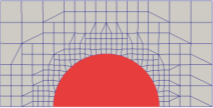
\includegraphics{flujometrias/shm_snapping.png}
        \caption{Snapping}
    \end{subfigure}
    \caption{Pasos de SnappyHexMesh\parencite{shm_steps}}\label{fig:openfoam_shm_pasos}
\end{figure}

El complemento \emph{blockMesh} crea una malla paramétrica con bloques, con
opciones para la creación de la malla con gradientes de tamaño de bloques y
diferentes opciones para los bordes, los cuales se pueden construir por líneas
rectas, arcos o
``splines''.\footnote{\url{https://doc.cfd.direct/openfoam/user-guide-v11/blockmesh}}
%
La malla se genera o configura con un diccionario \emph{blockMeshDict} ubicado
en \emph{constant/polyMesh}, con el cual se construye un cubo capaz de contener
la geometría del puerto a simular.

El complemento \emph{snappyHexMesh}
\footnote{\url{https://doc.cfd.direct/openfoam/user-guide-v11/snappyhexmesh}} es
el segundo paso del mallado.
%
Parte de una malla de bloques como la generada con la utilidad \emph{blockMesh}
y la \emph{talla} para acomodarse a la geometría dada, generando una malla 3D
conformada por hexaedros y hexaedros partidos a partir de superficies de caras
triangulares en formato de \emph{estereolitografía} (STL por sus siglas en
inglés).
%
Además permite refinar zonas particulares de la geometría y crear un
refinamiento mayor en la zona de la capa límite.
 \label{capitulo:3_openfoam} \pagebreak

\chapter{DESARROLLO} \label{capitulo:DESARROLLO}
% Los resultados obtenidos en cada uno de los pasos de este trabajo se detallan en
este capítulo, comenzando por el motor obtenido en la primer iteración de
optimización con el algoritmo genético y el modelo de CAD resultante.
%
Luego se muestran los resultados de las flujometrías realizadas a partir del
modelo de CAD, incluyendo las mallas obtenidas para algunos casos seleccionados
y el resultado detallado de algunas de las flujometrías, finalizando con el mapa
de $C_{D}$ obtenido, tanto para el puerto de admisión como para
el puerto de escape.

Por último se presentan los resultados de la segunda ronda de optimización con
el algoritmo genético, en la que se utilizó el mapa de $C_{D}$ obtenido en el
paso previo.
 \label{capitulo:4_desarrollo_iteracion} \pagebreak
Los resultados obtenidos en cada uno de los pasos de este trabajo se detallan en
este capítulo, comenzando por el motor obtenido en la primer iteración de
optimización con el algoritmo genético junto con el modelo de CAD generado.
%
Luego se muestran los resultados de las flujometrías realizadas a partir del
modelo de CAD, incluyendo las mallas obtenidas para algunos casos seleccionados
y el resultado detallado de algunas de las flujometrías, finalizando con el mapa
de $C_{D}$ obtenido, tanto para el puerto de admisión como para
el puerto de escape.

Por último se presentan los resultados de la segunda ronda de optimización con
el algoritmo genético, en la que se utilizó el mapa de $C_{D}$ obtenido en el
paso previo.

\section{Primer Iteración}
%
La primer optimización se realizó partiendo de una población al azar, con los
coeficientes de descarga constantes de 0.7 y 0.75 para el puerto de admisión y
escape respectivamente.
%
El algoritmo genético se ejecutó durante 100 generaciones con una población de
100 individuos y la función objetivo definida en la
sección~\ref{sec:funcion_objetivo} con los pesos indicados, operadores y
parámetros correspondientes indicados en la tabla~\ref{tab:config_genetico}.

\begin{table}[ht!]
  \centering
  \begin{tabular}{cc} \toprule
    Parámetro & Valor \\ \midrule
    RPMS & $1000\times[1, 2, 3, 4, 5, 6, 7, 8, 9]$ \\
    Pesos de función objetivo & $(1, 1, 1, 6, 8, 9, 8, 7, 7)$ \\
    Cantidad de ciclos de ICESym & 2 \\
    Diámetro mínimo & 0.05 \\
    Diámetro máximo & 0.1 \\
    Longitud mínima de tubo & 0.5 \\
    Longitud máxima de tubo & 2 \\
    Ángulo mínimo & 0 \\
    Ángulo máximo & 90 \\
    Separación angular máxima & 70 \\
    Tamaño de población & 100 \\
    Tamaño de torneo & 10 \\
    $\mu$ & 0 \\
    $\sigma$ & 1 \\
    $\alpha$ & 0.5 \\
    Probabilidad de cruza & 0.9 \\
    Probabilidad de mutación & 0.5 \\
    Cantidad de generaciones & 20 \\
    Tamaño de \emph{SALÓN DE LA FAMA} & 1 \\ \bottomrule
    \end{tabular}
  \caption{Configuración utilizada.}\label{tab:config_genetico}
\end{table}

% Para ICESym se utilizaron dos ciclos de simulación, por considerarse que es
% suficientemente preciso para esta primer aproximación.
% %
% En la figura XX se puede ver que a partir de la segunda iteración se obtienen
% buenos resultados, esto se debe a que los datos de partida para la segunda
% iteración, son los resultados de la primer iteración.
%
%
%

En la gráfica de evolución se observa  que se obtuvo rápidamente un individuo
con un puntaje relativamente alto en en las primeras iteraciones, el resultado
final tiene una aptitud 1.5 veces la aptitud media de la población de la última
generación, los parámetros que definen este candidato son los listados en la
tabla y se ilustran en la figura~\ref{fig:primer_op}.
%
Este motor tiene un rendimiento volumétrico máximo de $r_{v} \simeq 0.83$ para 2500
RPM y si bien la función objetivo favorece curvas suaves, se ven dos picos de
rendimiento en la curva, siendo el segundo con $r_{v} \simeq 0.79$ a 7500 RPM.

\begin{figure}
\begin{center}
  \begin{tabular}{rl}
    \begin{tikzpicture}[baseline, trim axis left]
      \begin{axis}[
        xlabel=Generación,
        ylabel=Puntaje,
    legend pos=south east,
        grid=both,
        ]
        \addplot table [x=Gen,y=Avg]{data/genetico.dat} ;
        \addplot table [x=Gen,y=Max]{data/genetico.dat} ;
        \legend{Media, Máximo}
      \end{axis}
    \end{tikzpicture}
    &
    \begin{tikzpicture}[baseline, trim axis right]
      \begin{axis}[
        xlabel=Velocidad del motor [RPM],
        yticklabel pos=upper,
        ylabel={$\eta_{v},x_{r}$},
        ylabel near ticks,
        grid=both,
        legend pos=south east,
        ]
        \addplot table [x=RPM,y=RendVol]{data/primer_rend_vol.dat} ;
        \addplot table [x=RPM,y=FracRes]{data/primer_rend_vol.dat} ;
        \legend{$\eta_{v}$, $x_{r}$ }
      \end{axis}
    \end{tikzpicture}
    \\
  \end{tabular}
\end{center}
\caption{Primer Iteración} \label{fig:primer_op}
\end{figure}

\begin{table}
  \centering
  \begin{tabular}{ccc} \toprule
    Parámetro & Valor & Unidad \\ \midrule
    DTA & 97.24 & mm\\
    DTE & 81.15 & mm\\
    LIT & 519.31 & mm\\
    LET & 976.66 & mm\\
    IIA & 1.12 & grado\\
    IFA & 70.15 & grado\\
    EIA & 85.14 & grado\\
    EFA & 11.13 & grado\\ \bottomrule
  \end{tabular}
  \caption{Mejor Candidato.}\label{tab:resultado_primer_it}
\end{table}

En la figura~\ref{fig:PoTi_primer_op} se muestran las curvas de potencia y
torque del motor, como es de esperarse se ve que ambas copian la curva de
rendimiento volumétrico, con una potencia indicada máxima de 230 HP a 9000 rpm y
un torque máximo de 210 N.m. a\ 7500 RPM.
NOTA: FALTA CORREGIR ESTA POTENCIA CON EL MODELO DE FLOR O DE KNOLL
% TODO
% NOTA: FALTA CORREGIR ESTA POTENCIA CON EL MODELO DE FLOR O DE KNOLL

\begin{figure}
  \begin{center}
  \begin{tikzpicture}
    \begin{axis}[
      xlabel=Velocidad del motor [RPM],
      ylabel={$P_{i}[HP],T_{i}[N.m.]$},
  legend pos=south east,
      grid=both,
      width={13cm}]
      \addplot table [x=RPM,y=PotInd]{data/primer_rend_vol.dat} ;
      \addplot table [x=RPM,y=PotNet]{data/primer_rend_vol.dat} ;
      \addplot table [x=RPM,y=TorqInd]{data/primer_rend_vol.dat} ;
      \addplot table [x=RPM,y=TorqNet]{data/primer_rend_vol.dat} ;
      \legend{Potencia Indicada, Potencia Neta, Torque Indicado, Torque Neto}
      \legend{$\dot{W}_{i,n,1}$,$\dot{W}_{freno,1}$ , $T_{i,1}$, $T_{freno,1}$}
    \end{axis}
  \end{tikzpicture}
  \end{center}
  \caption{Torque y Potencia de Primer Iteración} \label{fig:PoTi_primer_op}
\end{figure}


\section{Modelo de CAD}
%
A partir de los resultados obtenidos se realizó un modelo de CAD de los puertos
que se ilustra en la figura~\ref{fig:motor_cad1} y~\ref{fig:motor_cad2}.
%
Se representó solamente la mitad superior del motor que contiene ambos puertos
de admisión y escape, este modelo es paramétrico y permite rotar los componentes
del motor para obtener distintas posiciones del conjunto para generar la
geometría a evaluar.

% Algunos redondearon las aristas internas incluyendo las paletas y las puntas del rotor para favorecer el proceso de mallado, ya que los bordes agudos pueden ser problmeáticos para el mallador \emph{snappyHexMesh}.

\begin{figure}[ht]
  \centering
    \begin{subfigure}{0.4\textwidth}
        \centering
        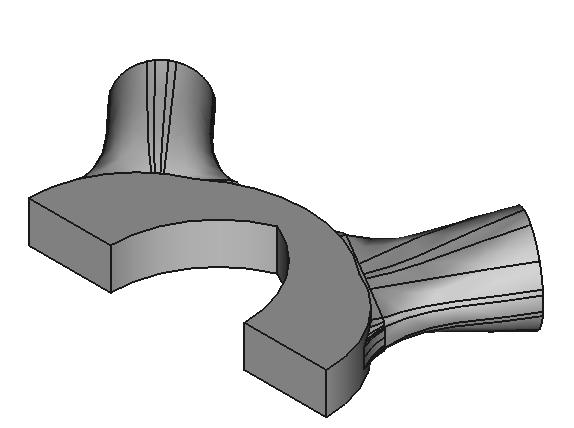
\includegraphics[width=\textwidth]{CAD/motor_cad1.png}
    \end{subfigure}
    \hfill
    \begin{subfigure}{0.4\textwidth}
        \centering
        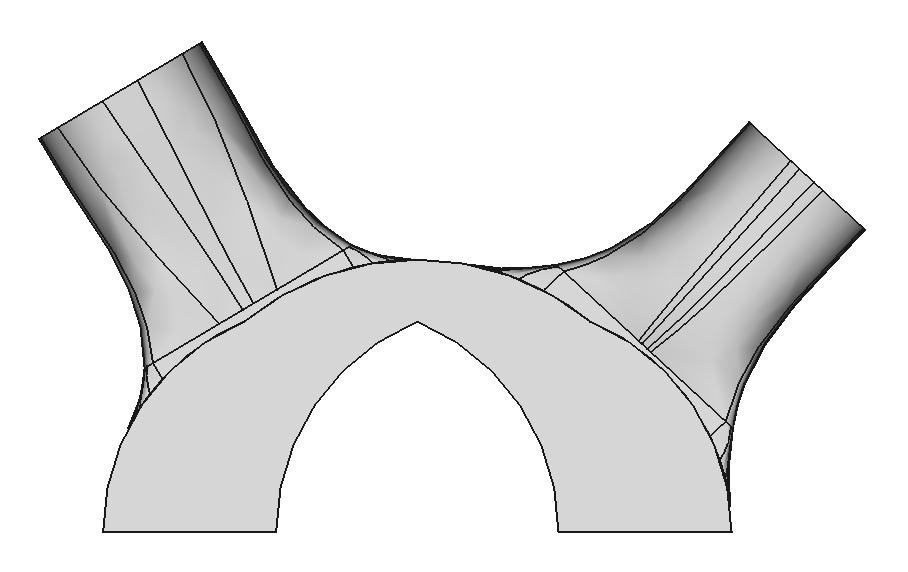
\includegraphics[width=\textwidth]{CAD/motor_cad2.png}
    \end{subfigure}
  \caption{CAD Primer Iteración}\label{fig:motor_cad1}
\end{figure}


\begin{figure}[ht]
  \centering
    \begin{subfigure}{0.8\textwidth}
        \centering
        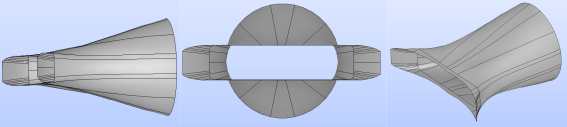
\includegraphics[width=\textwidth]{CAD/vistas_admision.png}
        \caption{Puerto de Admsisión.}
    \end{subfigure}
    \begin{subfigure}{0.8\textwidth}
        \centering
        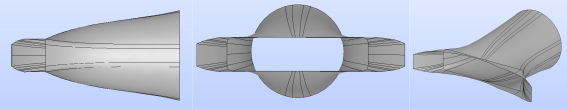
\includegraphics[width=\textwidth]{CAD/vistas_escape.png}
        \caption{Puerto de Escape.}
    \end{subfigure}
  \caption{CAD Primer iteración (vistas fuera de escala).}\label{fig:motor_cad2}
\end{figure}

La altura del puerto del lado de la cámara de combustión se mantuvo en dos
tercios del a altura de cámara $h_{p} = \frac{2}{3}h_{c}$, manteniendo el eje
central de cada puerto de forma que intersecte el centro del motor con el
propósito de eliminar una variable de la geometŕia a modelar.
%
El foco de esta etapa de optimización es el diámetro del puerto y el reglaje.
%
% Se generó uno de estos modelos para cada posición del cigueñal simulada en las
% fluojmetrías.

%%%%%%%%%%%%%%%%%%%%%%%%%%%%%%%%%%%%%%%%%%%%%%%%%%%%%%%%%%%%%%%%%%%%%%%%%%%%%%%
 \label{capitulo:4_primer_iteracion} \pagebreak
%%%%%%%%%%%%%%%%%%%%%%%%%%%%%%%%%%%%%%%%%%%%%%%%%%%%%%%%%%%%%%%%%%%%%%%%%%%%%%%
\section{Flujometrías}

De la pirmer iteración se obtuvo la geometría y datos de funcionamiento del
motor con esto se representó la curva de diferencia de presión en función de la
alzada del puerto obtenido a diferentes velocidades de giro del motor.
%
Utilizando esta gráficas se identificó puntos de mayor interés en los cuales
realizar las flujometrías.
%
% inicialmente se propusieron un total de XXX flujometŕias, sin embargo algunas
% combinaciones de $\l_{v}, \Delta P$ no se pudieron ejecutar hasta la
% convergencia del flujo másico, por lo que se redujo la cantidad de flujometrías
% final a xxx flujometrías, xxx para el puerto de admisión y xxx para el puerto
% de escape, el par  se detalla en la figura XXX y tabla xxx.
%
Los pares $(l_{v}, \Delta P)$ seleccionados para obtener el $C_{D}$ del puerto
se detallan en las figuras~\ref{fig:delta_p_admision}
y~\ref{fig:delta_p_escape}.
%
Inicialmente se propusieron 51 flujometŕias pudiendo realizar un total de 36
simulaciones que devoliveron 56 valores de $C_{D}$.

\begin{figure}[h]
  \centering
  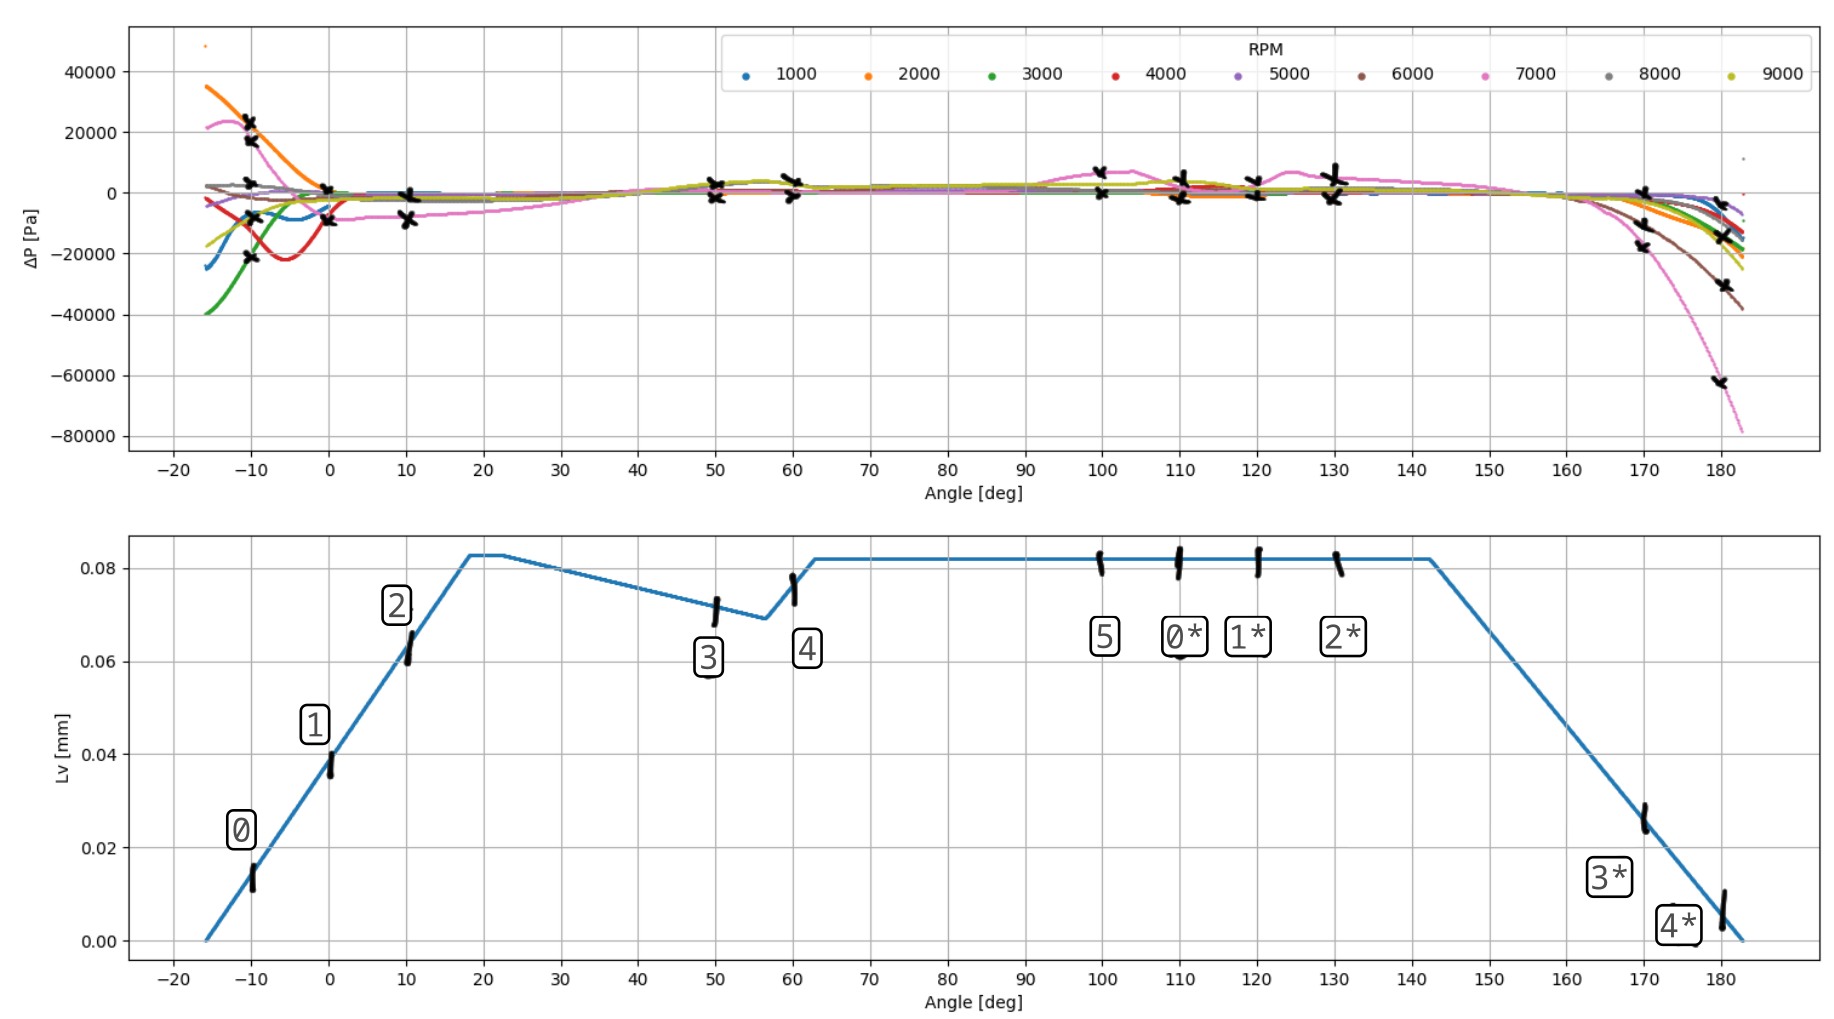
\includegraphics[width=\textwidth]{flujometrias/admision_delta_p_anot.png}
  \caption{Flujometrías puerto de admisión}\label{fig:delta_p_admision}
\end{figure}

\begin{figure}[h]
  \centering
  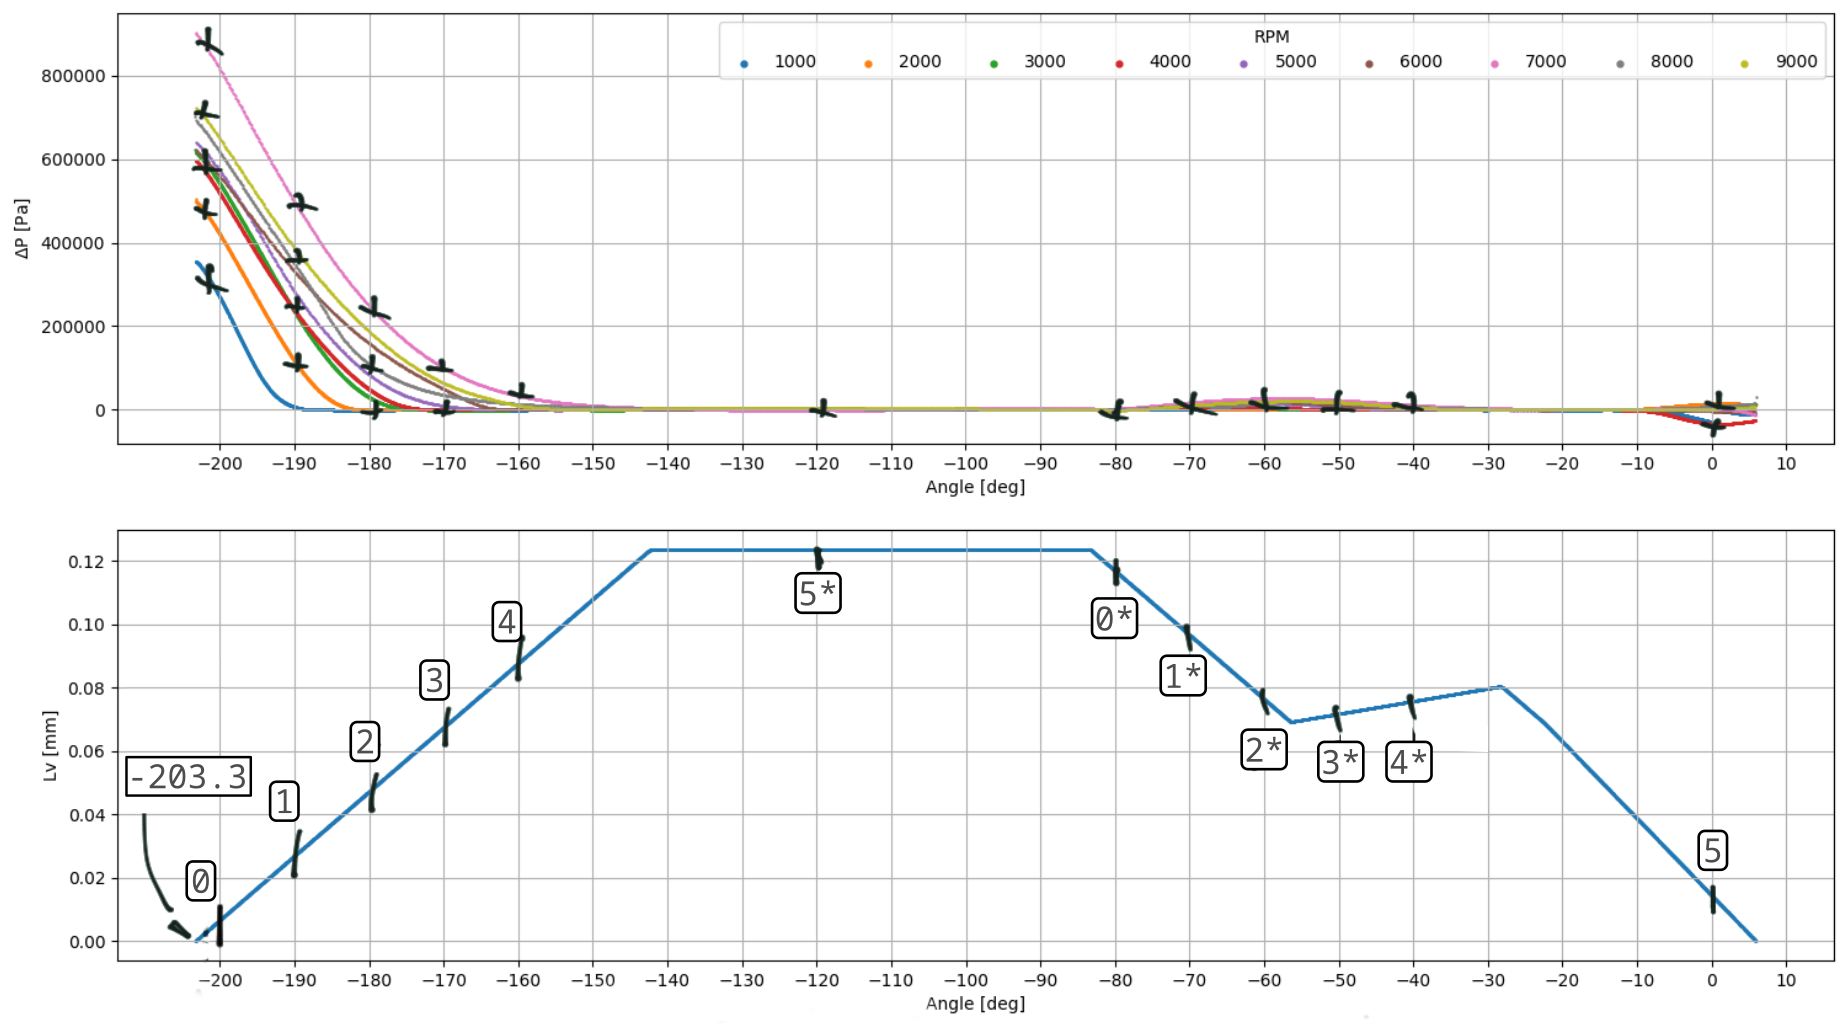
\includegraphics[width=\textwidth]{flujometrias/escape_delta_p_anot.png}
  \caption{Flujometrías puerto de escape}\label{fig:delta_p_escape}
\end{figure}


% \begin{table}[ht!]
%   \centering
%   \begin{tabular}{cccccc}\toprule
%     GRA/RPM & 1000 & 2000 & 3000 & 7000 & 9000 \\ \midrule
%     0       & -    & X    & -    & X    & - \\
%     10      & -    & -    & -    & X    & - \\
%     50      & -    & -    & X    & X    & X \\
%     100     & X    & -    & -    & X    & - \\
%     590     & X    & X    & X    & -    & - \\ \bottomrule
%   \end{tabular}
%   \caption{Flujometrías puerto de admisión}\label{tab:flujometrias_admision}
% \end{table}


% \begin{table}[ht!]
%   \centering
%   \begin{tabular}{cccccccc}\toprule
%     GRA/RPM & 1000 & 2000 & 3000 & 4000 & 7000 & 8000 & 9000 \\ \midrule
%     405     & X    & X    & -    & -    & X    & -    & X \\
%     410     & -    & X    & -    & X    & X    & X    & - \\
%     420     & -    & -    & -    & X    & -    & X    & - \\
%     430     & -    & X    & -    & -    & -    & -    & - \\
%     440     & X    & -    & -    & -    & X    & -    & X \\
%     500     & -    & -    & X    & -    & X    & X    & - \\ \bottomrule
%   \end{tabular}
%   \caption{Flujometrías puerto de escape}\label{tab:flujometrias_escape}
% \end{table}

Algunas flujometrías se realizaron en tres etapas, partiendo de una malla gruesa
con celdas de 15mm de tamaño inicial, culminando en celdas de 5mm.
%
En otros se realizó directamente la flujometría con mallas base de 5mm.

En general se simuló alrededor de 0.02 segundos de flujo  hasta alcanzar un
valor estable del caudal másico.
%
En la figura~\ref{fig:adm_10_7000rpm} se muestra el desarrollo de la simulación
en términos de $\dot{m}$ para el puerto de admisión con el cigüeñal en
$\theta=10^{\circ}$.
%
La línea anaranjada sobre el final de la simulación representa la poricón de
datos que se seleccionó para calcular el caudal másico, esto se realizó tomando
la media de los últimos n valores obtenidos.

\begin{figure}[ht]
  \centering
  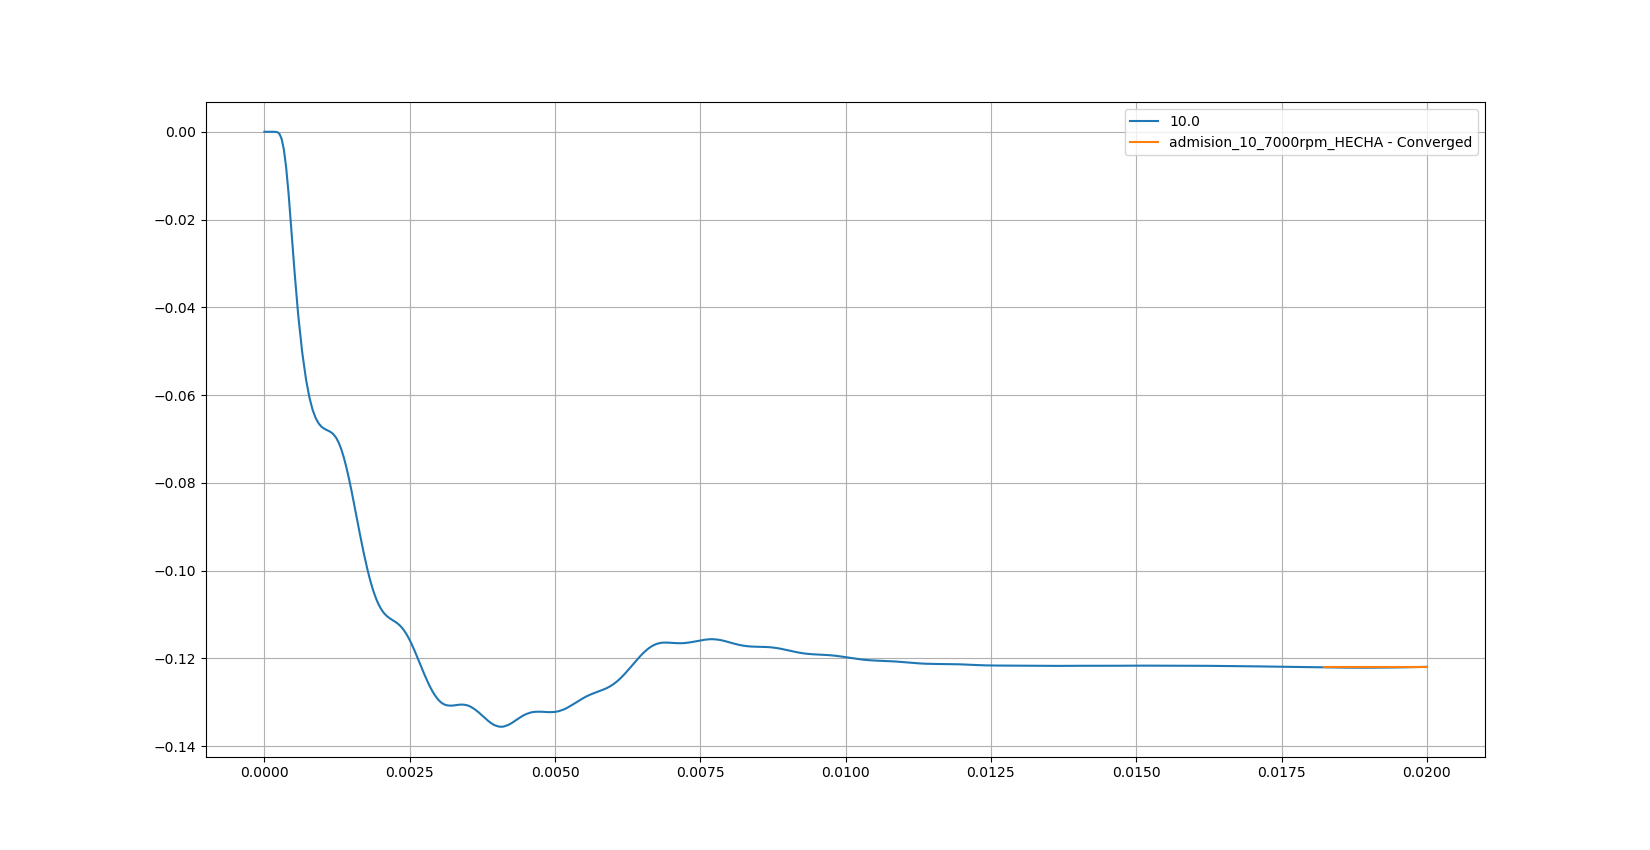
\includegraphics[width=\textwidth]{flujometrias/admision_SFV_10_0.png}
  \caption{Puerto de admisión 10º \@ 7000RPM}\label{fig:adm_10_7000rpm}
\end{figure}

Como se mencionó en el apartado~\ref{capitulo:DESARROLLO}, la modificaión
realizada a ICESym para funcionar con un mapa de $C_{D}$ dependiente de dos
variables requiere que los datos de entrada estén distribuidos en una grilla
rectangular.
%
A partir de las flujometrías realizadas se confeccionó el mapa de $C_{D}$, la
totalidad de puntos evaluados se presentan en las
tablas~\ref{tab:mapa_cd_admision} y~\ref{tab:mapa_cd_escape} para el puerto de
admisión y escape respectivamente.
%
Los datos obtenidos no forman una grilla rectangular, por lo que se utilizó
un método de suavizado de promedio móvil con $N=2$ para generar dicha grilla, el
resultado se ve en las figuras~\ref{fig:mapa_cd_admision}
y~\ref{fig:mapa_cd_escape}.

\begin{figure}[ht!]
    \centering
    \begin{subfigure}{0.7\textwidth}
        \centering
        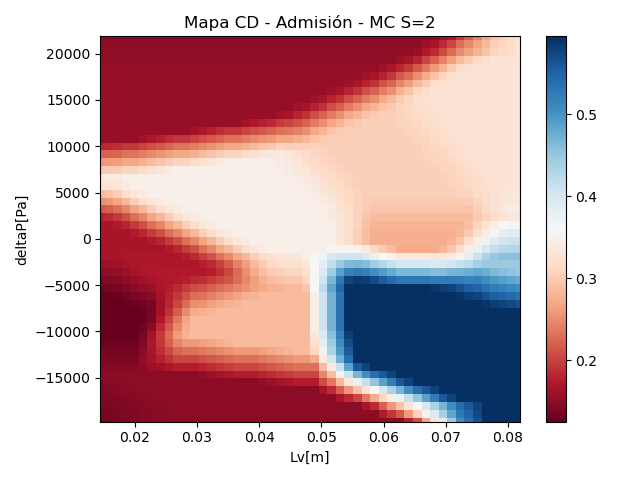
\includegraphics[width=\textwidth]{mapa_cd/mc_s2_mapa_adm.png}
        \caption{Puerto de admisión}\label{fig:mapa_cd_admisión}
    \end{subfigure}
    \hfill
    \begin{subfigure}{0.7\textwidth}
        \centering
        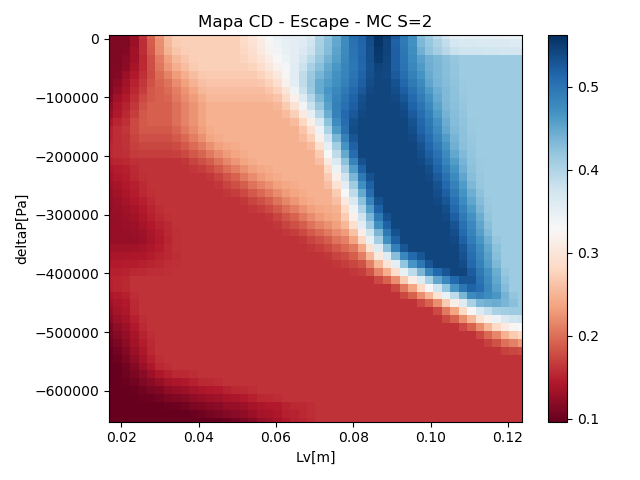
\includegraphics[width=\textwidth]{mapa_cd/mc_s2_mapa_esc.png}
        \caption{Puerto de escape}\label{fig:mapa_cd_escape}
    \end{subfigure}
    \caption{Mapas de $C_{D}$}\label{fig:mapa_cd_mc_s2}
\end{figure}

En el mapa del puerto de admisión se observa un máximo de $C_{D}\simeq 0.6$ para
para $l_{v}=62.95 mm$ y $\Delta P\simeq -7.37 KPa$, obteneniendo un flujo hacia
afuera del puerto de $0.122092 kg/seg$, este valor se obtiene para un
reflujo de gases residuales apenas abre el puerto de admisión, en particular
este valor se obtuvo para el el $10^{\circ}$ a 7000 RPM.
%
Las líneas de flujo para este caso se ven en la figura~\ref{fig:adm_cd_max}, las
líneas de corriente están coloreadas según el módulo de la velocidad y las
flechas indican el sentido de flujo.
%
Para este caso se ve que la mayor velocidad de flujo se da en el gas que sale de
la cámara de combustión residual que viene de descargar el gas al puerto de
escape habiendo algo de flujo de estos gases al puerto de admisión.
%
El menor valor también se obtiene para un valor muy próximo a la apertura del
puerto de admisión, siendo $C_{D}\simeq 0.12$ con un reflujo de
$\dot{m}\le 0.005$, $l_{v}=144.3 mm$ y $\Delta_{P}=-6.57 KPa$ para el puerto a
$590^{\circ}$ a 1000 RPM, las líneas de corriente para la flujometría de este
caso se ven en la figura~\ref{fig:adm_cd_min}.
%
En términos de flujo másico, el mayor valor  es de $\dot{m}=70 g/seg$ se da
durante un período de máxima apertura del puerto con $l_{v}=81.94 mm$ y
$\Delta_{P}=4.95 KPa$ siendo $C_{D}=0.32874$, la flujometría correspondiente se
ve en la figura~\ref{fig:adm_m_max}.


\begin{figure}[ht]
    \centering
    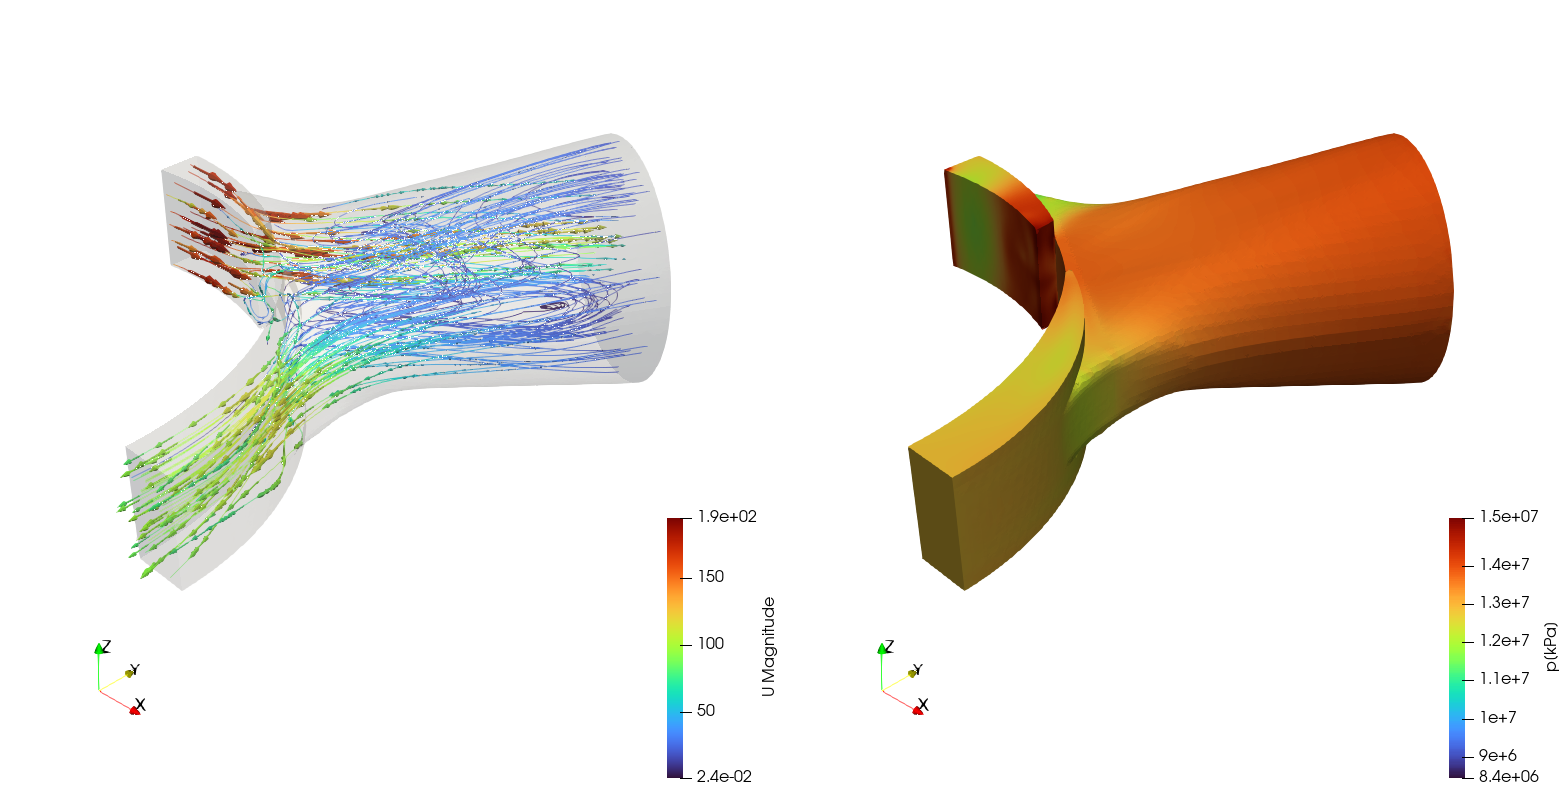
\includegraphics[width=\textwidth]{flujometrias/adm_cd_max.png}
    \caption{Admisión - Valor máximo de $C_{D}$}\label{fig:adm_cd_max}
\end{figure}

\begin{figure}[ht]
    \centering
    \includegraphics[width=\textwidth]{flujometrias/adm_cd_min.png}
    \caption{Admisión - Valor mínimo de $C_{D}$}\label{fig:adm_cd_min}
\end{figure}

\begin{figure}[ht]
    \centering
    \includegraphics[width=\textwidth]{flujometrias/adm_cd_max.png}
    \caption{Admisión - Valor máximo de $\dot{m}$}\label{fig:adm_m_max}
\end{figure}

Para el puerto de escape se observa el máximo $C_{D}=0.57686$ para
$l_{v}=87.76 mm$, $\Delta_{P}=-1 KPa$ con un flujo másico de $145 g/s$
hacia afuera para $440^{\circ}$ a 9000 RPM.
%
Las líneas de corriente para este caso se muestran en la
figura~\ref{fig:esc_cd_max}.

El máximo $C_{D, \max}=0.09631$ ocurre para $l_{v}=16.83 mm$ y
$\Delta_{P}=-652.9 KPa$, donde se encuentra el flujo bloqueado por la alta
diferencia de presiones alcanzando $\dot{m}=38.6 g/seg$, en la
figura~\ref{fig:esc_cd_min} se muestran las líneas de corriente para este caso.
%
El máximo valor de flujo másico es $\dot{m}=176.1 g/seg$ para $l_{v}=87.76 mm$ y
$\Delta_{P}=-334 KPa$, esto con el ciclo a $440^{\circ}$ y 7000 RPM, los
resultados de la flujometría se muestran en la figura~\ref{fig:esc_m_max}.

\begin{figure}[ht]
    \centering
    \includegraphics[width=\textwidth]{flujometrias/esc_cd_max.png}
    \caption{Escape - Valor máximo de $C_{D}$}\label{fig:esc_cd_max}
\end{figure}

\begin{figure}[ht]
    \centering
    \includegraphics[width=\textwidth]{flujometrias/esc_cd_max.png}
    \caption{Escape - (CAMBIAR POR CD MIN) Valor mínimo de $C_{D}$}\label{fig:esc_cd_min}
\end{figure}

\begin{figure}[ht]
    \centering
    \includegraphics[width=\textwidth]{flujometrias/esc_m_max.png}
    \caption{Escape - Valor máximo de $\dot{m}$}\label{fig:esc_m_max}
\end{figure}


\begin{table}
  \centering
    \begin{tabular}{cccc} \toprule
      Caso  & lv        & $\Delta P$    & $C_{D}$   \\ \midrule
      0     & 0.016826  & -100331.39    &  0.213882 \\
      0     & 0.106775  & 5723.72       &  0.489375 \\
      0     & 0.016826  & -263797.72    &  0.011021 \\
      0     & 0.106775  & -3296.18      &  0.803197 \\
      0     & 0.016826  & -652902.78    &  0.011106 \\
      0     & 0.106775  & -9613.29      &  0.815804 \\
      0     & 0.016826  & -513568.73    &  0.011280 \\
      0     & 0.106775  & -3232.97      &  0.813186 \\
      1     & 0.026960  & -116996.12    &  0.375219 \\
      1     & 0.096641  & -3643.9       &  0.878414 \\
      1     & 0.026960  & -237724.11    &  0.018632 \\
      1     & 0.096641  & -6684.11      &  0.867774 \\
      1     &  0.02696  & -496509.46    &  0.111212 \\
      1     &  0.09664  & -18256.20     &  0.805830 \\
      1     & 0.026960  & -237724.11    &  0.022716 \\
      1     & 0.096641  & -6684.11      &  0.862647 \\
      2     & 0.047228  & -49343.47     &  0.541857 \\
      2     & 0.076373  & -5712.86      &  0.918061 \\
      2     & 0.047228  & -109348.67    &  0.487137 \\
      2     & 0.076373  & -17090.38     &  0.914182 \\
      3     & 0.067496  & 13.83         &  0.696967 \\
      3     & 0.071759  & -134.24       &  0.707263 \\
      3     & 0.067496  & -100073.52    &  0.731100 \\
      3     & 0.071759  & -24077.34     &  0.723965 \\
      4     & 0.075750  & -11793.31     &  0.946392 \\
      4     & 0.087764  & -33418.12     &  0.235717 \\
      4     & 0.087764  & -10715.70     &  0.221632 \\
      4     & 0.075750  & -5167.81      &  0.897169 \\
      6     & 0.123601  & -73.94        &  0.878522 \\ \bottomrule
    \end{tabular}
  \caption{Mapa de $C_D$ del puerto de escape} \label{tab:mapa_cd_escape}
\end{table}

\begin{table}
  \centering
  \begin{tabular}{cccc} \toprule
      Caso  & lv        & $\Delta P$    & $C_{D}$   \\ \midrule
      0     & 0.014432  & -6574.97      &  0.206543 \\
      0     & 0.081937  & -87.24        &  0.828822 \\
      0     & 0.014432  & 21856.29      &  0.243975 \\
      0     & 0.081937  & -573.65       &  0.738459 \\
      0     & 0.014432  & -19738.67     &  0.222406 \\
      0     & 0.081937  & 519.60        &  0.487115 \\
      0     & 0.081937  & 1571.95       &  0.587277 \\
      0     & 0.014432  & 18077.97      &  0.256415 \\
      0     & 0.014432  & 2668.61       &  0.247292 \\
      0     & 0.081937  & 0.98          &  0.025970 \\
      2     & 0.062951  & -297.79       &  0.816487 \\
      2     & 0.081937  & 292.92        &  0.466147 \\
      2     & 0.062951  & -7374.88      &  0.980617 \\
      2     & 0.081937  & 4953.85       &  0.541619 \\
      3     & 0.071763  & 4092.13       &  0.501641 \\
      3     & 0.025832  & -3689.81      &  0.289852 \\
      4     & 0.069767  & -789.00       &  0.615690 \\
      4     & 0.069767  & 7869.92       &  0.599348 \\
      4     & 0.005564  & -12539.15     &  0.534555 \\
      4     & 0.005564  & -10091.84     &  0.583979 \\ \bottomrule
    \end{tabular}
  \caption{Mapa de $C_d$ del puerto de Admisión} \label{tab:mapa_cd_admision}
\end{table}

La geometría obtenida luego de realizar la optimización con los mapas de $C_D$
incorporados a la simulación de ICESym se muestra en la figura \ref{fig:geom_nueva}.
%
Se puede ver que la geometría es similar a la inicial, siendo el puerto de
admisión algo menor en cuanto a diámetro que en el caso inicial.
%
Como es de esperarse, incorporar estos mapa al modelo del motor tiene un efecto
en el comportamiento del mismo, esto se puede observar principalmente en las
curvas de presión del motor.

Para obtener el mapa se tomaran valores de flujo másico en las combinaciones de
$(\Delta P, l_v)$ que están indicadas en la tabla~\ref{tab:casos}.
%
Como se ve en la Figura~\ref{fig:flujometrias}, los puntos a evaluar son los
listados en la Tabla~\ref{tab:casos}.
%
El mapa de $C_D$ obetnido a partir de las flujoemtrías se lista en la
tabla~\ref{tab:mapaAdm} y~\ref{tab:mapaEsc} para los mapas de admisión y escape
respectivamente.
%
% En la figura \ref{fig:flujometrias} se ve que se eligieron más cantidad de
% muestreos en las zonas donde hay mayores cambios de presión.
%
% La figura \ref{fig:flujometrias} fué obtenida a partir de los resultados del
% simulador ICESym, restando para las velocidades seleccionadas la presión de la
% cámara a la presión en la boca del puerto.

\begin{figure}
    \centering
    \includegraphics[width=1\textwidth]{flujometrias_admision.png}
    \caption{Flujometrías para el puerto de Admisión}\label{fig:flujometrias}
\end{figure}

\begin{table}
    \centering
    \begin{tabular}{rll} \toprule
        Caso & Ángulos  & Velocidades (rpm) \\ \midrule
        0    & -10, 110 & 1000, 2000, 3000, 7000, 8000 \\
        1    & 0, 120   & 2000, 7000 \\
        2    & 10, 130  & 2000, 7000 \\
        3    & 50, 170  & 3000, 7000, 9000 \\
        4    & 60, 180  & 3000, 5000, 6000, 7000 \\
        5    & 95       & 1000, 7000\\ \bottomrule
    \end{tabular}
    \caption{Flujometrías a realizar}\label{tab:casos}
\end{table}


\begin{table}
  \parbox{.45\linewidth}{
  \centering
  \begin{tabular}{rccc}\toprule
    Item & $L_v[m]$ & $\Delta P[Pa]$ & $C_D$ \\ \midrule
    \lua{tex.print(mapaCd(myData.admision))}
    \bottomrule
    \end{tabular}
  \caption{Mapa $C_D$ del puerto de Admisión}\label{tab:mapaAdm}
  }
\hfill
\parbox{.45\linewidth}{
  \centering
  \begin{tabular}{rccc}\toprule
    Item & $L_v[m]$ & $\Delta P[Pa]$ & $C_D$ \\ \midrule
    \lua{tex.print(mapaCd(myData.escape))}
    \bottomrule
    \end{tabular}
  \caption{Mapa $C_D$ del puerto de Escape}\label{tab:mapaEsc}
}
\end{table}
 \label{capitulo:4_flujometrias} \pagebreak
\section{Segunda iteración y resultado final}
%
En la segunda iteración se utilizó el mapa de $C_D$ para la admisión y escape
como dato de entrada de ICESym, con esto se realizó una serie de corridas de
optimización con el algoritmo genético, de las cuales se seleccionaron los
mejores candidatos.
%
Se obtuvieron 3 candidatos principales, indicados como \emph{$run_{34}$},
\emph{$run_{38}$}, \emph{$run_{51}$} cuyas geometrías se indican en la
tabla~\ref{tab:2iter_geom}, se ve que los diámetros son similares y que la mayor variaión
se dan en los largos de los conductos de admisión y escape.
%
Exceptuando la corrida $run_{51}$ los ángulos de apertura de los puertos de
admisión se mantienen cercanos figura \ref{fig:2iter_general}.
%
Para determinar cuál de todos es el más promoetedor, se compararon las curvas de
presión, torque y potencia, las cuales se muestran en la
figura~\ref{fig:PoTi_segunda_op}.

\begin{table}
\centering
\begin{tabular}{ccccccccc} \toprule
  Corrida & DTA  & DTE  & LIT    & LET    & IIA   & IFA   & EIA   & EFA \\
  -       & mm   & mm   & m      & m      & gra   & gra   & gra   & gra \\ \midrule
  run 34  & 83,2 & 100  & 0,6839 & 1,2323 & 5,81  & 52,26 & 81,29 & 8,71 \\
  run 38  & 83,2 & 96,1 & 1,1226 & 1,1226 & 0     & 52,26 & 87,1  & 8,71 \\
  run 51  & 84,5 & 81,9 & 0,6839 & 0,3548 & 17,42 & 55,16 & 66,77 & 37,74 \\
\end{tabular}
\caption{Geometrías de segunda iteración}\label{tab:2iter_geom}
\end{table}

\begin{figure}[ht]
  \centering
  \begin{subfigure}[b]{.5\textwidth}
    \centering
    \includegraphics{gnuplot/segunda_iter_pot.pdf}
    \caption{Potencia indicada y al freno} \label{fig:primer_op}
  \end{subfigure}%
  \begin{subfigure}[b]{.5\textwidth}
    \centering
    \includegraphics{gnuplot/segundo_rend_vol.pdf}
    \caption{Rendimiento Volumétrico}
  \end{subfigure}
    \caption{Segunda Iteración} \label{fig:primer_op}
\end{figure}


El motor tiene una potencia máxima de 117 CV a las 6500 RPM y un par máximo de
177Nm a 4000 RPM, este coincide con el máximo de rendimiento volumétrico de
$\sim 0.845$
%
En la figura~\ref{fig:PoTi_segunda_op} se nota los efectos del coeficiente de
descarga en la simiulación del motor, esto se ve comparando los resultados de la
primer iteración con coeficientes de descarga constantes a la segunda con el
mapa de $C_{D}$ en función de presión y velocidad de operación del motor.

\begin{figure}[ht]
  \centering
  \includegraphics{gnuplot/comparativa.pdf}
  \caption{Comparativa de Torque y potencia al freno} \label{fig:PoTi_segunda_op}
\end{figure}
 \label{capitulo:4_segunda_iteracion} \pagebreak


\chapter{CONCLUSIONES} \label{capitulo:5_conclusiones}
Se ha obtenido un prediseño de los sistemas de admisión y escape que buscó
maximizar el rendimiento volumétrico y reducir la fracción de gases residuales
en un rango medio a medio alto de revoluciones del motor, obteniendo una curva
de rendimiento volumétrico con una sintonía a 2000 RPM y manteniendo valores de
$\eta_v$ cercanos al 70\% para 6000 a 7000 RPM.
%
Además, se obtuvo un mapa de $C_D$ que modeliza el funcionamiento de los
puertos con apertura de puerto y diferencia de presión como variables.

Junto con estos resultados se desarrolló un conjunto de \emph{scripts} que
permiten utilizar el simulador ICESym como una \emph{caja negra}, pudiendo
configurar, ejecutar y leer los resultados de una simulación, esto permite
utilizar el simulador acoplado a otro programa.

Como trabajos a futuro se tiene la incorporación de los modelos de fricción
obtenidos en trabajos anteriores\parencite{roldan} a ICESym, la creación de un
optimizador genético híbrido, es decir, que permita utilizar algoritmos
genéticos para determinar los puntos más interesantes del dominio evaluado para
un problema dado y el uso de técnicas directas para encontrar el valor del
óptimo buscado.
 \label{capitulo:5_conclusiones} \pagebreak

\chapter{REFERENCIAS}
\printbibliography[heading=none] \pagebreak

\chapter{ANEXO I}


 
 \pagebreak

\end{document}
